\documentclass[a4paper,11pt]{article}
%% Language and font encodings
\usepackage[utf8]{inputenc}				% Package description
\usepackage[english]{babel}				%
\usepackage[T1]{fontenc}				%

%% Useful packages
\usepackage[nottoc,chapter]{tocbibind}
\usepackage[dvipsnames,table]{xcolor}			% Add colors
\usepackage[margin=2cm]{geometry}		% Adjust margin
\usepackage[pdftex]{hyperref}			% Styling of links
\usepackage{tipa}						% International Phonetics Alphabet
\usepackage[scaled]{helvet}
\usepackage{enumitem}
\usepackage{titling}
\usepackage{arydshln}
\usepackage{graphicx}
\usepackage{csquotes}
\usepackage{pgfgantt}
\usepackage{rotating}
\usepackage[graphicx]{realboxes}
\usepackage{pdflscape} 					% provides the landscape environment.
\usepackage{afterpage} 					% provides coloring of entire page.
\usepackage{amsmath} 					% relates to math
\usepackage{amsfonts} 					% font for math
\usepackage[nomain,acronym,xindy,toc,automake,nonumberlist]{glossaries} 			% for glossary
\usepackage{nameref}
\usepackage{textcomp}					% Celcius
\usepackage[sorting=none,style=apa,backend=biber,hyperref=true,backref=true,]{biblatex}
\usepackage{float}
\usepackage{listings}
\usepackage{caption}
\usepackage{quoting}
\usepackage{nameref}
\usepackage[bottom]{footmisc}
\usepackage[compact]{titlesec}
\usepackage{longtable}
\usepackage{xpatch}
\usepackage{caption}
\usepackage{pxfonts}
\usepackage{makecell}
\usepackage{afterpage}








% Load default font
\renewcommand\familydefault{\sfdefault}
\renewcommand{\arraystretch}{1.3}

% Colors
\definecolor{Red}{RGB}{226,0,21}
\definecolor{Fuchsia}{RGB}{185,2,118}
\definecolor{Violet}{RGB}{80,36,127}
\definecolor{LightViolet}{RGB}{204,153,255}
\definecolor{DarkBlue}{RGB}{0,86,145}
\definecolor{DarkGray}{RGB}{82,95,107}
\definecolor{LightBlue}{RGB}{0,142,207}
\definecolor{Turquoise}{RGB}{0,168,176}
\definecolor{LightGreen}{RGB}{120,190,32}
\definecolor{DarkGreen}{RGB}{0,98,73}
\definecolor{Black}{RGB}{0,0,0}

% Glossary style
\setglossarystyle{altlist}

% Quoting style
\quotingsetup{vskip=0.5pt}

% Caption style
\captionsetup[table]{font=footnotesize}
\captionsetup[figure]{font=footnotesize}
\captionsetup[equation]{font=footnotesize}

% Fix f in math mode
\newcommand{\f}{\mkern-2mu f\mkern-3mu}


% Depth of TOC
\setcounter{tocdepth}{2}

% Prevent inspringen alinea
\setlength\parindent{0cm}
\setlength\parskip{0.7em}

% Prevent large empty area above multiline equations and images
\xapptocmd\normalsize{%
\abovedisplayskip=-12pt 
%\abovedisplayshortskip=0pt 
%\belowdisplayskip=0pt 
%\belowdisplayshortskip=0pt
}{}{}

% Spacing in lists
\setlist[enumerate]{topsep=0pt,itemsep=2pt,partopsep=1ex,parsep=2pt}

% Use different main color for each document:
% Violet = Research plan

% Style of links
\hypersetup{
colorlinks = true, 
linkcolor = DarkBlue, 
urlcolor = DarkBlue,
citecolor = DarkBlue}

% Spacing around sections
\titlespacing{\section}{0pt}{*0}{*0}
\titlespacing{\subsection}{0pt}{*4}{*0}
\titlespacing{\subsubsection}{0pt}{*2}{*0}
\titlespacing{\paragraph}{0pt}{*0}{*0}
\titlespacing{\subparagraph}{0pt}{*0}{*0}

% Section
\titleformat{\section}
{\normalfont\huge\bfseries\centering\color{document}}{\thesection}{1.0em}{}

% Subsection
\titleformat{\subsection}
{\normalfont\Large\bfseries}{\thesubsection}{1.0em}{}

% Subsubsection
\titleformat{\subsubsection}
{\normalfont\large\bfseries}{\thesubsubsection}{1.0em}{}

% Paragraph
\titleformat{\paragraph}[hang]
{\normalfont\normalsize\bfseries}{\theparagraph}{1.0em}{}

% Subparagraph
\titleformat{\subparagraph}[hang]
{\normalfont\normalsize\bfseries}{\thesubparagraph}{1.0em}{}

% Quotes
\AtBeginEnvironment{quote}{\itshape}


% New page after new section
\newcommand{\sectionbreak}{\clearpage}

% Style for title page
\DeclareRobustCommand{\change}{%
  \color{white}%
}
\DeclareRobustCommand{\stopchange}{%
  \normalcolor
}

% Style for code section
\definecolor{codegreen}{rgb}{0,0.6,0}
\definecolor{codegray}{rgb}{0.5,0.5,0.5}
\definecolor{codepurple}{rgb}{0.58,0,0.82}
\definecolor{backcolour}{RGB}{242,242,242}

\renewcommand\lstlistingname{Code sample}
\captionsetup[lstlisting]{font={footnotesize}}

\lstset{
    backgroundcolor=\color{backcolour}, 
    commentstyle=\color{DarkGreen},
    keywordstyle=\bfseries\color{Violet},
    numberstyle=\tiny\color{codegray},
    stringstyle=\color{codepurple},
    basicstyle=\ttfamily\footnotesize,
    breakatwhitespace=false,         
    breaklines=true,                 
    captionpos=b,                    
    keepspaces=true,                 
    numbers=left,                    
    numbersep=5pt,                  
    showspaces=false,                
    showstringspaces=false,
    showtabs=false,  	
    tabsize=3,
    belowskip=1em,
    aboveskip=1em,
    float,
    floatplacement=h,
    firstnumber=1
}

\lstdefinelanguage{SHACL}{
	morekeywords={select,prefixes,sparql,sh,path,severity,minCount,message,property,datatype,pattern,targetClass,maxCount,NodeShape,a,Violation,class,or,Info},
	morecomment=[l][\color{DarkGreen}]{\#}
}

\lstdefinelanguage{GDOL}{morekeywords={pattern,Class,DataProperty,ObjectProperty,InverseRelation,DisjointClasses,SubClassOf,Domain,Range,targetClass,Violation,then,ontology,logic,OWL,Ontology,end,and,then},
	morecomment=[l][\color{DarkGreen}]{\%\%}
}

\lstdefinelanguage{SPARQL1}{
	morekeywords={SELECT,WHERE,GROUP,ORDER,BY,FILTER,DISTINCT,COUNT,UNION,PREFIX,AS,STRSTARTS,STRENDS,SUM,HAVING},
	morecomment=[l][\color{DarkGreen}]{\#}
}

\lstdefinelanguage{SHACLSPARQL}{
	morekeywords={select,prefixes,sparql,sh,path,severity,minCount,message,property,datatype,pattern,targetClass,maxCount,NodeShape,a,Violation,class,or,Info,SELECT,WHERE,GROUP,ORDER,BY,FILTER,DISTINCT,COUNT,UNION,PREFIX,AS,STRSTARTS,STRENDS,SUM,HAVING},
	morecomment=[l][\color{DarkGreen}]{\#}
}


\newcommand\blankpage{
    \null
    \thispagestyle{empty}
    \addtocounter{page}{-1}
    \newpage
    }
\makeglossaries
\makeindex

\newglossaryentry{control_system}
{
name=control system,
description={A control system is able to influence the behaviour of devices or (sub)systems}
}
\newglossaryentry{strategy}
{
name=strategy,
description={A strategy is generally defined as a method or plan to achieve a specific goal or solve a specific problem, where as an algorithm is generally defined as a mathematical or logical specification of how to solve one or multiple problems. An algorithm could be considered being a strategy to reach a specific goal, or solve a specific problem.}
}

\newglossaryentry{goal}
{
name=goal,
description={A control system is build to solve a problem or, from a different perspective, reach a specific goal. In order to reach that goal, the control system (and it's connected devices) consumes energy.}
}

\newglossaryentry{hybrid_system}
{
name=hybrid system,
description={In the context of this study a hybrid system is a system which uses a combination of hardware and software to reach a specific system state.}
}

\newglossaryentry{overhead_consumption}
{
name=overhead,
description={Overhead is consumed by the control system itself, but at the same time it does not contribute to a specific goal. It equals the total amount of energy consumed by the system minus the specific amount of energy that is consumed to reach a specific goal}
}

\longnewglossaryentry{renewable_energy}
{
name=renewable energy
}
{
Energy from renewable sources is defined by \cite{RE1} as: 
\begin{quote}energy from renewable sources’ means energy from renewable non-fossil sources, namely wind, solar, aerothermal, geothermal, hydrothermal and ocean energy, hydropower, biomass, landfill gas, sewage treatment plant gas and biogases;\end{quote}
}
\newglossaryentry{problem_instance}
{
name=problem instance,
description={Each problem can have several instances, depending on the environment in which the problem needs to be solved.}
}

\newglossaryentry{environment}
{
name=environment,
description={The environment (of the system) cannot be influenced by the system itself. Examples: the weather, the amount of people in a room.}
}

\newglossaryentry{system_state}
{
name=system state,
description={The system state can be influenced by the system itself, either directly (by controlling connected devices and sensors) or indirectly (by using the impact of the connected devices and sensors). Examples: (direct) switching on a pump, (indirect) increasing the temperature of a room.}
}

\newglossaryentry{primary_energy_sources}
{
name=primary energy sources,
description={\parencite{IM9} considers crude oil, natural gas, biomass and waste, coal, wind, solar, hydro-power, geothermal-power and ocean-power, and nuclear power (based on natural uranium) as \emph{primary energy sources}.}
}
\addbibresource{../../BIB_Articles_SM.bib}
\addbibresource{../../BIB_Articles_KM.bib}
\addbibresource{../../BIB_Articles_PM.bib}
\addbibresource{../../BIB_Articles_ME.bib}
\addbibresource{../../BIB_Articles_DM.bib}
\addbibresource{../../BIB_Articles_SO.bib}
\addbibresource{../../BIB_Articles_BR.bib}
\addbibresource{../../BIB_Articles_SMW.bib}
\addbibresource{../../BIB_Articles_CON.bib}
\addbibresource{../../BIB_Articles_THE.bib}
\addbibresource{../../BIB_Articles_ODP.bib}
\addbibresource{../../BIB_Articles_BI.bib}
\addbibresource{../../BIB_Online.bib}
\addbibresource{../../BIB_Books.bib}
\addbibresource{../../BIB_Other.bib}
%% Commands
\makeglossaries
\sloppy

%% Document shared data
\newcommand{\version}{2.00}

%% Define document colorscheme
\colorlet{document}{Violet}
\colorlet{documentText}{white}

% Include research questions
% Title
\newcommand{\researchname}{a decision design pattern to detect and present the maturity-level of decision-relevant information}

% Main research question
\newcommand{\researchquestion}{$RQ$: To what extent can the detection of premature information using SHACL Semantic Web constraints contribute to evidence-based decision-making?}

% Help = too vague.
% Increase, reduce = needs to be measurable.
% Motivate = keyword that needs to be clearly defined.

% Validation
\newcommand{\valone}{$VAL1$: To what extent can the detection of premature information using SHACL Semantic Web constraints contribute to evidence-based requirements prioritisation?}
\newcommand{\valtwo}{$VAL2$: To what extent can the detection of premature information using SHACL Semantic Web constraints contribute to evidence-based alternative solution selection?}

% Theoretical framework
\newcommand{\tfone}{$TF1$: How are decision-makers making decisions?} % Evidence-based management, information is never complete. Which types of decisions? Binary, numeric?
\newcommand{\tftwo}{$TF2$: When is decision-relevant information premature?} % Completeness and reliability of information. Depends on the context.
\newcommand{\tfthree}{$TF3$: To what extent can we detect premature information?} % semantic web, application logic. How can Semantic Web technologies practically interact with application logic?
\newcommand{\tffour}{$TF4$: What is the impact of the presentation of the information maturity-level on a decision?} % Visualization of information. Show impact of the decision on the information?
\newcommand{\tffive}{$TF5$: To what extent can we generalise our approach?} % Ontology / UI Design patterns 

% Data structuur
\newcommand{\rqdsone}{$DS1$: To what extent can we create a generic ontology design pattern for evidence-based management?}
\newcommand{\rqdstwo}{$DS2$: To what extent can we store the information completeness and reliability in an (extended) evidence-based management ontology?}
\newcommand{\rqdsthree}{$DS3$: To what extent can we use Semantic Web inferencing, consistency, and constraints to detect premature information?}

% Visualization
\newcommand{\rqvisone}{$PRES1$: How do we define the maturity-level of decision-relevant information?}
\newcommand{\rqvistwo}{$PRES2$: Under which circumstances is a decision-maker interested in the maturity-level of decision-relevant information?}
\newcommand{\rqvisthree}{$PRES3$: To what extent can we make it easier for a decision-maker to understand the maturity-level of decision-relevant information?}


% Actual document content
\begin{document}
\begin{titlepage} 
\pagecolor{document}\afterpage{\nopagecolor}

\begin{center}
\change

% Title
\textsc{ \Huge\bfseries\centering\color{white} \researchname}\\[0.5cm] % Title of your document

% Fill the rest of the page with whitespace
\vspace*{\fill} 

% Document data

\begin{table}[!htbp]
\color{white}
\begin{tabular}{ p{5cm}  p{10cm} }
Written by: & Mario Verhaeg \\
Student ID number: & 851210638 \\
Thesis presentation date: & June 30, 2020 \\
Version: & \version, \today \\
Degree program: & Faculty Science, Open University of the Netherlands \\
& Computer Science Master's program \\
Course: & IM0004 CS Graduation Assignment Preparation\\
& IM990C Computer Science Graduation Assignment \\
Thesis supervisor: & dr. L.W. Rutledge \\
Second reader: & dr. Bastiaan Heeren \\
\end{tabular}
\end{table}
\stopchange
\end{center}
\end{titlepage}

%\begin{center}

%----------------------------------------------------------------------------------------
%	TITLE SECTION
%----------------------------------------------------------------------------------------
 
{\Huge\bfseries\centering\color{document} Document history}\\[0.5cm] % Title of your document

\end{center}
\begin{table}[!htbp]
\centering
\begin{tabular}{| p{2cm} | p{2cm} | p{11cm} |}
\hline
Version & Date & Description \\
\hline
1.0 & 2019-08-30 & The schedule is adjust to match the methodology. Several risks were added. \\
\hdashline
1.01 & 2019-10-27 & The schedule is updated. \\
\hdashline
1.02 & 2019-12-27 & The schedule is updated. \\
\hdashline
1.03 & 2020-04-11 & The schedule is updated. The description of the progress and my personal experiences have been extended up to April 2020. \\
\hdashline
1.04 & 2020-04-xx & ... \\
\hline
\end{tabular}
\caption{Document history}
\label{table:history}
\end{table}
\vspace*{\fill} 
\newpage
\thispagestyle{empty}
\begin{center}
\textsc{\normalfont\Huge\bfseries\color{document}Acknowledgement} 
\end{center}
Studying has been a significant part of my life since I started with this journey in 2011. In the meantime, I started working at Bosch, the German industrial giant and moved to the south of Germany. This job challenges me every day and brings me to exciting parts of the world. It was quite a challenge to keep this up for almost ten years, but I made it. 

My initial goal was to finish this study before my 30\textsuperscript{th} birthday. Unfortunately, I was not able to achieve this goal. At the same time, the learning experience was more important for me than keeping the schedule. I have no regret from restarting several courses, including the graduation assignment, and taking my time to understand what is going on. My goal is to learn, not to impress.

The inspiration for the subject of this graduation assignment came from my work environment. I observed that we made several complex and high-impact decisions using information that was based on opinions and open for interpretation. Taking the complexity of the job, product, and market into account, I felt there should be a more structured approach to take these decisions. We, Lloyd and I, discussed the potential to use the Semantic Web to address parts of this challenge, which intrigued me.

Even though they are probably responsible for messing up my schedule, staying close to my family and friends contributed to this result. The everyday distractions they caused, the weekends travelling to the Netherlands driving 160km/h on the autobahn for six hours, the long Oktoberfest weekends, and the countless trips to the Alps kept me alive during these ten years. Lloyd kept me focused during the graduation assignment itself, and provided a continuous stream of guidance during our regular appointments, while Bastian shared his outside-in perspective. Finally, effective tooling also helps. Skype only failed me once in the last couple of months, Grammarly improved my writing skills, and Spotify shared countless hours of motivation. 

Thank you for your support.

Mario

\vspace*{\fill} 
\newpage
\thispagestyle{empty}
\begin{center}
\textsc{\normalfont\Huge\bfseries\color{document}Abstract} 
\end{center}
\newcommand{\abstractkey}{This work proposes to use a combination of Semantic Web concepts, including consistency, inferencing, and constraints to detect premature information. We calculate the information maturity-level and present it using well-known data presentation concepts. We propose the decision design pattern to reduce the time and expertise domain experts need to build Semantic Web-based ontologies that can detect premature information and present the information maturity-level. Additionally, the transparent information maturity-level helps decision-makers to move from intuition-based decision-making to evidence-based decision-making.}

\abstractkey 

% Samenvatting, maximaal 200 woorden
Decisions, especially in the software product management discipline, are mostly complex and made based on intuition due to missing information or the lack of time to analyse the available information. A software product manager can understand if \emph{this} is the right time to make \emph{that} decision by understanding the information maturity-level of the decision-relevant information.

The decision design pattern calculates the information maturity-level using the completeness, reproducibility, consensus, and conflict violations. We detect the completeness, reproducibility, consensus, and conflict violations using Semantic Web constraints. Domain experts can re-use the decision design pattern and apply it for their decisions. Based on the presentation of the information maturity-level, the decision-maker can decide to continue the decision-making process or elaborate on the information.
 
We need to have the domain knowledge to validate the Semantic Web constraints. Therefore, we use two decisions from the software product management domain to validate our approach: requirement prioritisation and alternative solution selection. We create a supporting ontology structure for both decisions and instantiate the decision design pattern.

\noindent\textsc{\normalfont\large\bfseries\color{document}Key terms} \hfill \break
Evidence-based management; EBM; generic ontology design pattern; GODP; software product management; SPM; decision making; ontology design pattern; constraints; SHACL; Semantic Web.  

\vspace*{\fill} 


\newpage

\renewcommand{\baselinestretch}{0.40}\normalsize
\thispagestyle{empty}
\tableofcontents
\renewcommand{\baselinestretch}{1.0}\normalsize

% Research Planning
\section{Introduction} \label{introduction}
% Environment of the challenge
A software product manager needs to act as a spider in a web and is involved in many disciplines, for example, product lifecycle management, product requirements engineering, release planning, road mapping, and defining the product vision \parencite{PM02}. Keeping track of the sheer volume of information involved in these disciplines is a challenge. On top of that, in today's rapidly changing and uncertain environment, making strategic decisions has become increasingly complex \parencite{DM01}. The overall complexity of software product management leads to the identification of premature decision-making as one of the prime challenges in software product management \parencite{PM04}. 

\subsection{The prime challenge}
% The challenge
Practitioners are forming communities \parencite{WEB01} that share experience on, for example, \href{https://www.mindtheproduct.com/2018/10/evaluating-experiments-when-the-numbers-lie/}{"Evaluating Experiments: When the Numbers lie"} and \href{https://www.mindtheproduct.com/2019/01/how-can-enterprise-product-managers-attain-maximum-insight-from-limited-datapoints/}{"How can Enterprise Product Managers Attain Maximum Insight from Limited Datapoints?"}. The scientific community starts to investigate the feasibility of evidence-based decision-making in software product management, and recognises product managers need evidence-based decision-making for long-term and sustainable software product development \parencite{PM04}. At the same time, product managers are afraid that evidence-based decision-making reduces flexibility by formalising the decision-making process. Although the feasibility of evidence-based decision-making is still unclear, existing literature shows that the data related to, for example, sales and pricing, is available but not used for decision-making.
\begin{quoting}\itshape
'We are collecting a lot of data, but simply not using it...' \parencite{PM04}
\end{quoting}

Requirements prioritisation is an example that we analyse in more detail. Imagine a large multi-national organisation that sells an enterprise management software product. This organisation  stores information in different systems. These systems store customer-related information: the backlog management system stores the source of a requirement and the problem the customer faces, the CRM system stores the interactions with customers, and the ERP system stores revenue related information. It is very time-consuming to structure this information in a way it supports the decision-making process. Imagine this organisation sells multiple products to the same customer, and the organisation uses a different backlog management system for each product. Storing this information in various systems increases the complexity even further. At the same time, the decision-making process is complex and involves multiple stakeholders. Those stakeholders all have a different view on a situation. 

Unfortunately, this study cannot fully solve this challenge. We define a general data structure to store evidence-based information and use this structure to detect premature information and present the information maturity-level. The presentation of the information maturity-level helps the decision-maker to evaluate if the quality of the information used as a basis for the decision is acceptable. The decision-maker, a human being, is eventually responsible for making the (strategic) decision.

\subsection{Context}
% Bridge between problem and solution: Semantic Web
The challenge touches several disciplines in which researchers are active: decision-making, knowledge management, and for validation purposes, (software) product management. \cite{DM07} describe a theory on evidence-based decision-making that concludes that the decision-making process is not purely rational. Evidence can come from multiple (non-scientific) sources and is interpreted differently among persons. Knowledge management influences the decision-making process by, for example, the structure in which organisations store knowledge \parencite{KM03}. The scientific community gives little attention to decision-making processes \parencite{PM04}. Additionally, it is not always clear to software product managers what information could serve as evidence.

\subsection{Semantic web}
% Why is the Semantic Web relevant in this problem context?
Software product managers seem to be lacking insights into \emph{actionable} information: information that they should use to drive decisions. The Semantic Web promises to deliver actionable information:
\begin{quoting}\itshape
'The Semantic Web is a Web of actionable information...' \parencite{SM13}
\end{quoting}
The Semantic Web transforms meaningless and unstructured information into evidence that decision-makers can use in a specific context. This study uses the Semantic Web to store decision-relevant information into an evidence-based management structure. It uses inferencing, consistency, and constraints on top of this structure to detect premature information and calculate the information maturity-level of decision-relevant information. We generalize our approach and create several ontology design patterns that domain experts can re-use to solve similar challenges in a different context.

\subsection{Main research question}
\abstractkey

\begin{center}
\large\color{document}{\researchquestion}
\end{center}

\subsection{Approach}
The decision design pattern includes the evidence-based management pattern, the decision ontology pattern, and the decision presentation pattern. We create the evidence-based management pattern to prepare existing ontologies for evidence-based decision-making. The decision ontology pattern provides the structure to detect premature information. Last, the decision presentation pattern calculates the information maturity-level and presents it to the decision-maker. We use Semantic Web consistency, inferencing, and constraints. We validate the decision design pattern using two software product management decisions:
\begin{enumerate}
\item \nameref{val-rp}
\item \nameref{val-as}
\end{enumerate}
We instantiate parts of the decision design pattern in the context of these decisions. The instantiated patterns detect if decision-relevant information is premature. We calculate and present the information maturity-level in a way the software product manager can make the decision, or elaborate further on the decision-relevant information to increase the information maturity-level.
\section{Theoretical framework} \label{theoreticalframework}
The goal of the theoretical framework is to summarise the existing knowledge on the subjects related to the (main)research question. These questions define the scope of the theoretical framework:
\begin{itemize}[label={}]
\item \tfone
\item \tftwo
\item \tfthree
\item \tffour
\item \tffive
\end{itemize}
%=================================================================================================================================================================================================

\subsection{Decision making: science or art?} \label{tf_ebm}
We typically use prior experience, intuition, or advice from others to make decisions \parencite{DM12}. However, making a professional decision that might impact colleagues and customers is typically more challenging. We need to convince our stakeholders with the right arguments. Evidence-based management classifies these arguments. \cite{DM03} define evidence-based management as:
\begin{quote}\itshape
"Making decisions through the conscientious, explicit, and judicious use of four sources of information: practitioner expertise and judgment, evidence from the local context, a critical evaluation of the best available [external]research evidence, and the perspectives of those people who might be affected by the decision." \parencite{DM03}
\end{quote}

\subsubsection{Decision-making model} \label{tf_dmm}
Figure \ref{fig:dmm01} presents a mixed-level model for evidence-based decision-making. This model shows that a decision-maker bases a decision on multiple evidence types. The size of the circle represents the amount of influence the evidence type has in a specific decision.

\begin{figure}[H]
\centering
  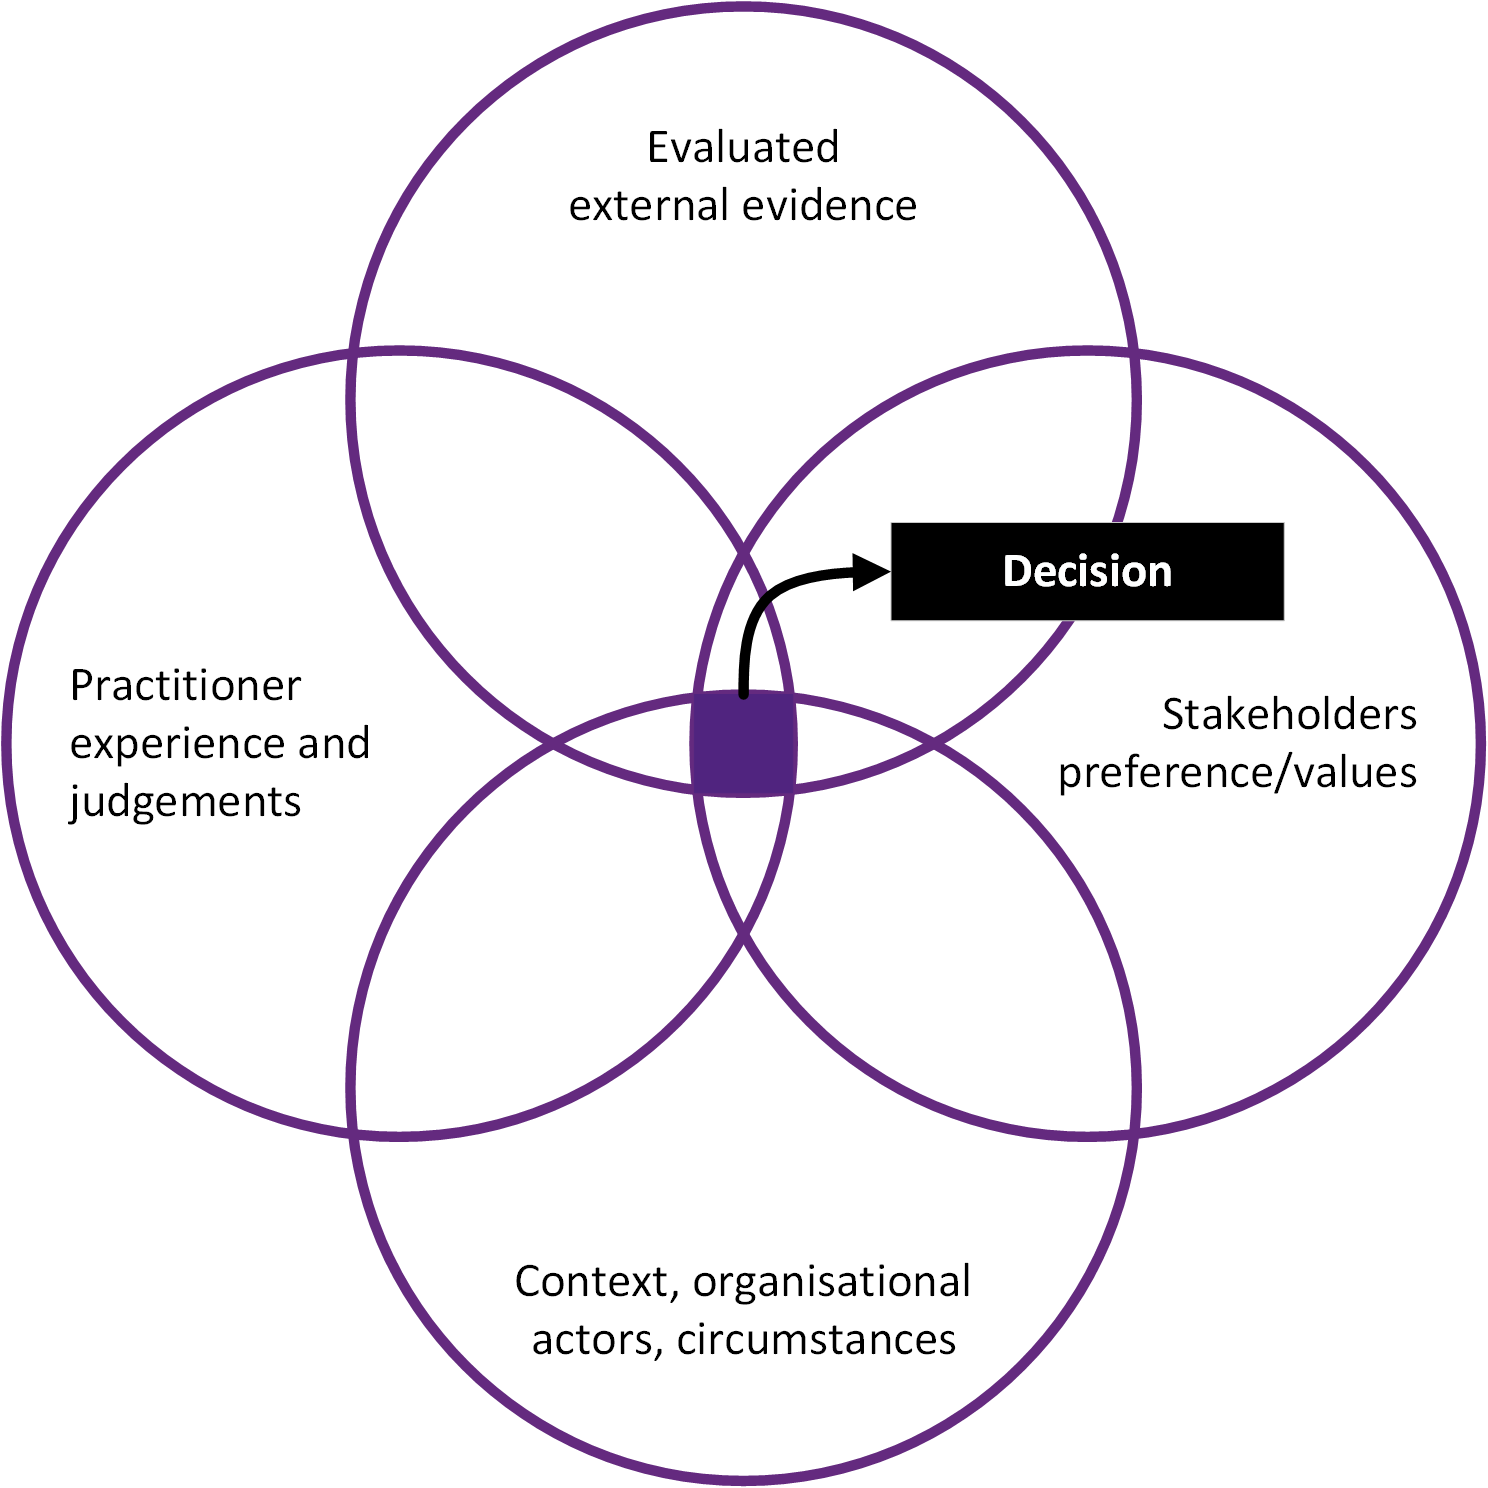
\includegraphics[width=8cm]{../../Images/DM07_Evidence.png}
  \caption{The four elements of evidence-based management \parencite{DM03}. The size of each circle (representing the strength of its influence) varies with each decision. For example, if we move the context, organisational actors, and circumstances further to the bottom, its influence in the decision decreases.}
  \label{fig:dmm01}
\end{figure}

Evidence includes local context\footnote{The context for individuals is given by the organisation and the context for the organisation is given by the external environment \parencite{DM04}.}, insight from other sources, and professional experience (or \textit{"accumulated past experience"} \parencite{PM04}) \parencite{DM03}. Different people use evidence types in different ways, depending on their personal experience. \cite{DM07} argue that evidence-based decision making is influenced by:
\begin{quoting}\itshape
"[...] managers' preferences and values as well as stakeholders' preferences within institutional, organisational and individual contexts." \parencite{DM07}.
\end{quoting}

Evidence-based decision-making considers the way decision-makers gather the evidence, ensure this suits the usage of the evidence (methodological fit), and the context in which the information used \parencite{DM07}. The quality of the information depends on its reproducibility, the transparency on evidence conflicts, and the consensus of evidence.

\subsubsection{Technology-driven knowledge management}
A knowledge management strategy represents how organisations have implemented knowledge management and how it impacts the firm's decision making \parencite{KM03}. The knowledge management strategy approach structures organisational knowledge to justify strategic choices (or decisions) and can save time in the decision-making process. 

%=================================================================================================================================================================================================
\subsection{Detecting premature information}
We use Semantic Web technologies to detect premature information. 

\subsubsection{Resource description framework schema (RDFS)}
Linking information starts with creating a \emph{common understanding} of the data concepts between different contexts: this is the goal of the Resource Description Framework (RDF) \parencite{SM13}. RDF Schema (RDFS) provides data-modelling mechanisms on top of RDF, allowing it to describe groups of related resources and the relationships between those resources \parencite{WEB06}. 

\subsubsection{SPARQL Query Language for RDF}
The SPARQL query language can query data stored in an RDFS data model. SPARQL can be considered a data-access and filtering protocol for RDFS \parencite{WEB08}. SPARQL uses a table to present its output (or result set). SPARQL can be used to test data in RDFS graphs by defining constraints in SPARQL and observing the output.

SPARQL queries can select data from an ontology. If a query returns with an empty result set, the constraints described in the $WHERE$ clause of query do not match any information in the ontology. This mechanism led to SPIN \parencite{WEB13}, also known as SPARQL rules. SPIN can attach SPARQL queries to classes. The SPARQL query would define the constraints that each instance of the class needs to satisfy. \cite{SM34} submitted SPIN to the W3C. However, SPIN never made it to a recommended standard. 

\subsubsection{Web Ontology Language}
The Web Ontology Language (OWL) can be used on top of RDF(S) to increase the expressivity in the relationships between data fields. Its main goal is to \emph{represent} knowledge \parencite{WEB04}. While RDF(S) describes the data and its relationships within a single ontology, OWL allows relationships between multiple ontologies and their data fields and supports various types of inference. Inferencing makes it easier to discover relationships between fields and reveal complexity in a structure that was not visible before \parencite{SM13}. 

The consistency on an OWL ontology can be checked by a reasoner, for example, Pellet. A reasoner includes consistency checkers based on the OWL specification \parencite{SM32}:
\begin{quote}\itshape
'An OWL consistency checker takes a document as input and returns one word being Consistent, Inconsistent, or Unknown.' \parencite{WEB12}
\end{quote}

Semantic web inferencing and reasoning works based on rules defined in OWL. The reasoner derives new facts from these rules. For example, the \emph{Super Property Of (Chain)} allows defining a chain of relationships; for example, $customer\_bought\_product\_from\_manufacturer$ is a combination of two relationships: $manufacturer\_produces\_product$ and $product\_bought\_by\_customer$. When these two relationships are defined, the reasoner automatically infers the super property (figure \ref{fig:superproperty}). Inferencing decreases the risk of mistakes and increases the completeness of the information. As a result, inferencing decreases the risk the decision-relevant information does not meet the expected requirements.

\begin{figure}[H]
\centering
  
\includegraphics[width=17cm]{../../Images/Superproperty.png}
  \caption{A super property that defines a chain of object properties. For example, the super property $customer\_bought\_product\_from\_manufacturer$ relates manufacturers with customers using the object properties $manufacturer\_produces\_product$ and $product\_bought\_by\_customer$.}
  \label{fig:superproperty}
\end{figure}

\subsubsection{Semantic web rule language (SWRL)}
\cite{SM35} attempted to introduce data validation mechanisms in the context of the Semantic Web. SWRL extends OWL with Horn-like rules that are a form of implication between an antecedent and consequent: whenever the antecedent is true, the consequent should be true as well. SWRL never made it past its W3C submission state. Semantic Web reasoners are also able to infer new knowledge based on SWRL rules.

\subsubsection{Shapes constraints language (SHACL)} \label{tfshacl}
OWL suffers from restrictions related to the limited possibilities for structural validation, and the built-in nature of the so-called \emph{Open World Assumption}\footnote{The open world assumption prevents a negation as failure that means that the absence of information cannot lead to any conclusion, but results in an \emph{unknown} evaluation.} \parencite{SM22}. Another limitation of OWL relates to the way how restrictions are working. For example, a person \emph{p} can only have one father, but \emph{p} has two individuals defined as a father. OWL assumes that these two values are representing the same real-world entity.

The W3C has accepted SHACL (Shapes Constraint Language) as a recommendation in 2017 \parencite{WEB05} to address these limitations. The main goal of SHACL is the \emph{validation} of RDF(S) graphs against a set of conditions by defining SHACL shapes \parencite{WEB05}. Figure \ref{fig:shacl1} presents SHACL conceptually. SHACL can detect data quality issues \parencite{SM23} based on the definition of constraints. For example, each person needs to have precisely one last name.  

\begin{figure}[H]
\centering
  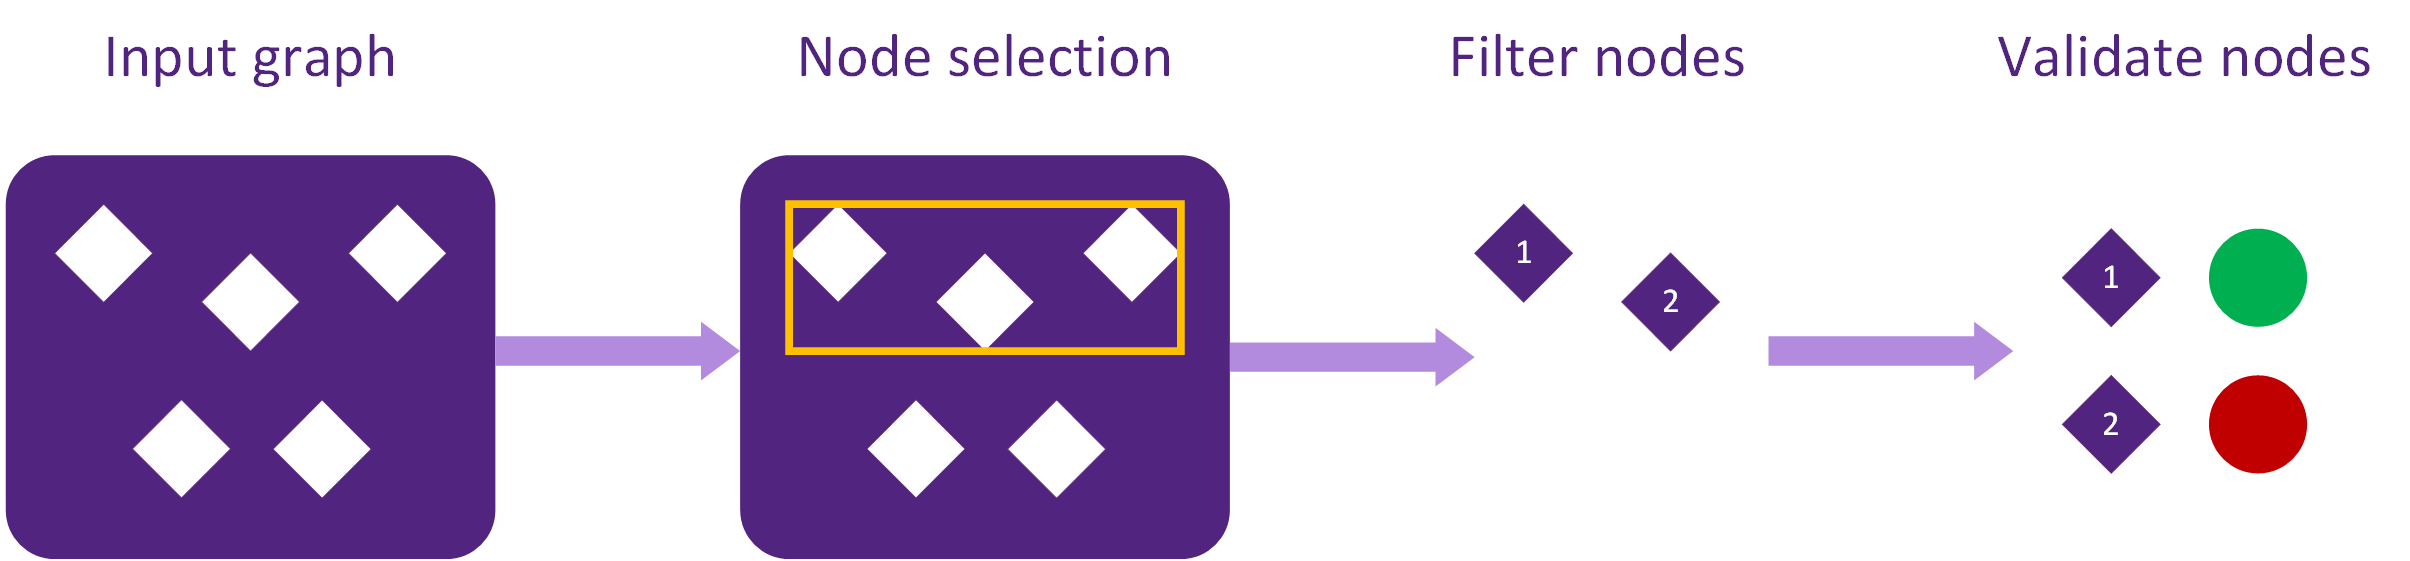
\includegraphics[width=15cm]{../../Images/SHACL1.png}
  \caption{The main goal of SHACL is the \emph{validation} of RDF(S) graphs against a set of conditions by defining SHACL shapes \parencite{WEB05}.}
  \label{fig:shacl1}
\end{figure}

%=================================================================================================================================================================================================
\subsection{Transformation of information into decisions} \label{tf_transformation_of_information}
The way a decision support system presents information to a user has a significant impact on the quality of that system \parencite{BI03}. Decision-makers can use the information as a communication medium, a knowledge management tool, and a decision support instrument \parencite{BI02}. We focus on the presentation of information as a decision-support instrument using graphs and charts. The presentation of information into graphs and charts enhances the capabilities of a decision-maker to process information \parencite{BI06}. However, each decision has its challenges. Selecting the wrong graph, chart, or navigation structure might lead to misleading conclusions. Therefore, the presentation needs to take the characteristics of the decision and the decision-maker into consideration \parencite{BI02}.

There are several ways to tailor the presentation of the information to the characteristics of a decision. First, we need to select the right chart type. The available chart types include, for example, scattergraphs, line graphs, bar graphs, and pie charts (\cite{BI09}, \cite{OTH09}). A pie chart is, for example, especially useful to make it easy to understand relative proportions. A (geographical) map can make it easier to understand data that is related to multiple locations.  Figure \ref{fig:visualisation_pattern} presents an example in which multiple charts are combined. The combination of charts is especially useful when the information that a decision-maker uses to make a decision contains geographical information \parencite{OTH09}.

\begin{figure}[H]
\centering
  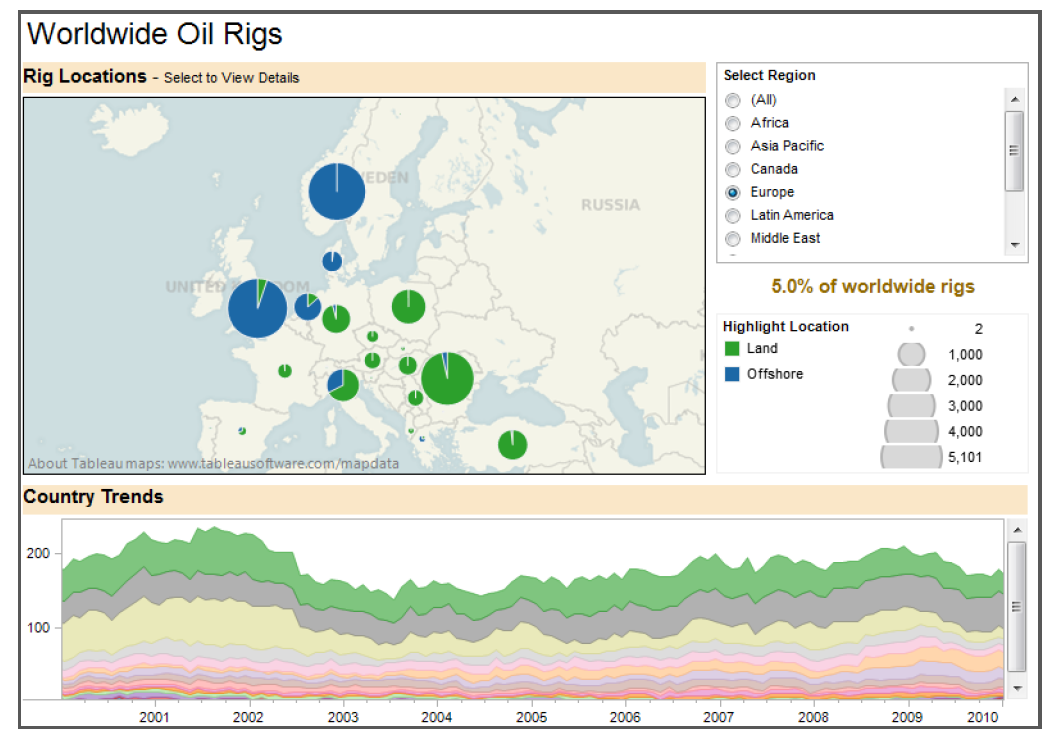
\includegraphics[width=12cm]{../../Images/02_TF_Visualisation_Pattern.png}
  \caption{The worldwide oil rigs using a combination of pie charts, a geographical map, and a line chart \parencite{OTH09}.}
  \label{fig:visualisation_pattern}
\end{figure}

Once we have selected a chart, we can tailor the chart itself. We can, for example, change the way the data markers and data labels are presented \parencite{BI09}. Figure \ref{fig:tf_good_chart} presents an example of a chart that is easy to interpret by the limited amount of information. It is consistently coloured, and the axis titles are explicit. Figure \ref{fig:tf_bad_chart} presents an example of a chart that is more difficult to interpret by the significant difference in scales, the inconsistent colouring, and the missing definitions of the axis'.

\begin{figure}[H]
\centering
  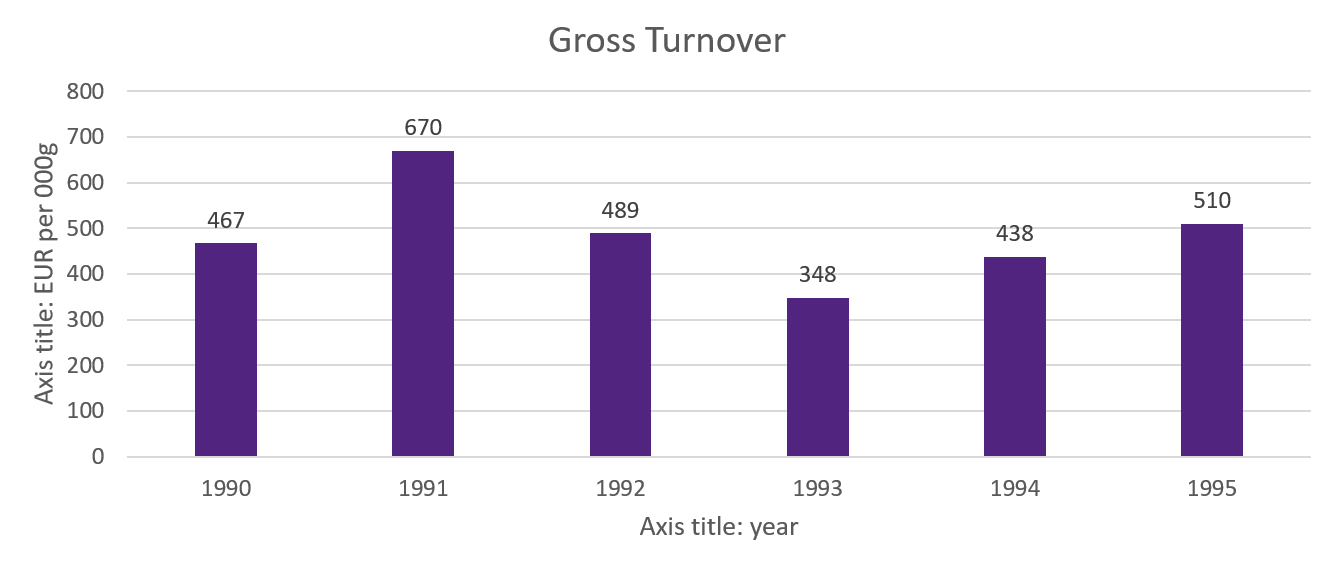
\includegraphics[width=13cm]{../../Images/02_TF/02_TF_Good_Chart.png}
  \caption{An example of a chart that is easy to interpret by the limited amount of information. It is consistently coloured, and the axis titles are explicit \parencite{BI09}.}
  \label{fig:tf_good_chart}
\end{figure}

\begin{figure}[H]
\centering
  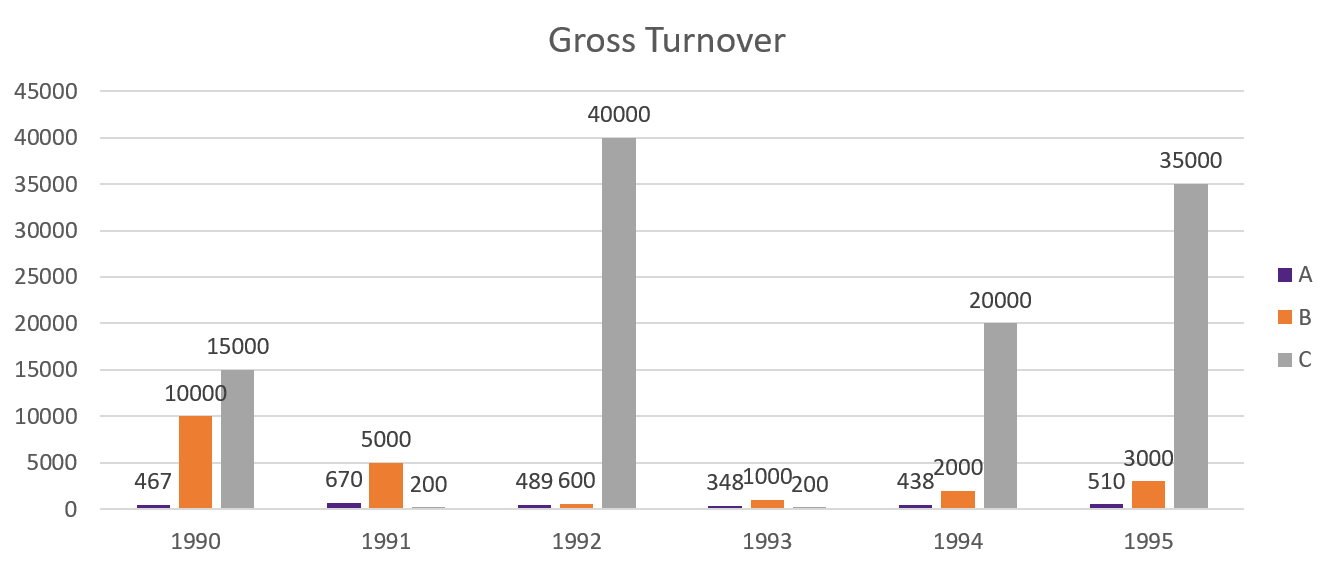
\includegraphics[width=13cm]{../../Images/02_TF/02_TF_Bad_Chart.png}
  \caption{An example of a chart that is more difficult to interpret by the significant difference in scales, the inconsistent colouring, and the missing definitions of the axis' \parencite{BI09}.}
  \label{fig:tf_bad_chart}
\end{figure}

\cite{BI09} describes best practices that are useful when we want to present information with a specific goal. For example, we should limit the usage of 3D charts as they tend to obliterate data series and are challenging to interpret. 

%=================================================================================================================================================================================================
\subsection{Generalisation}
\cite{BK03} defines a design pattern as the core of a solution for similar problems. Ontologies describe concepts on a knowledge level and focus on the structure of knowledge \parencite{SM19}. Presentation design patterns are challenging to find. However, we can interpret existing data presentation concepts like design patterns. These presentation concepts are reusable for similar problems as well.

\subsubsection{Ontology design patterns} \label{tf_odp}
\newcommand{\tfodp}{We define an ontology design pattern as an ontology configuration that effectively solves multiple problems \parencite{ODP06}.}

\tfodp

There are three types of stakeholders involved in ontology engineering \parencite{ODP02}: ontology experts, domain experts, and end-users. In general, end-users have little domain knowledge, domain experts have little ontology expertise, and ontology experts have little domain knowledge. Domain experts drive the majority of ontology development with limited involvement of ontology experts. This limited involvement might result in poor design choices \parencite{ODP02}. Ontology design patterns enable domain experts to re-use design decisions and best practices. 

\paragraph{Content ontology design patterns} \label{CODP}
A content ontology design pattern includes the generic use case, specific use-case, address logic, reference ontologies, formal relationships, sensitive axioms, and the related class diagram. This approach follows software design patterns that typically also contains a problem description, suggested solution, implementation guidelines and consequences of using the pattern \parencite{ODP07}.

\paragraph{Generic ontology design patterns} \label{GODP}
\cite{ODP06} introduced ontology design patterns in 2003. However, their adoption by ontology engineers has been slow \parencite{ODP02}. Ontology engineers have two options to use a predefined ontology design pattern:
\begin{enumerate}
\item Import the ontology design pattern as-is into an existing ontology. The import process might require some manual adjustments.
\item Manual redesign of the ontology design pattern, so it fits into the target ontology.
\end{enumerate}

The ontology design pattern clutters the ontology with information that might not be needed. Additionally, the ontology design pattern might introduce inconsistencies into the ontology related to, for example, naming conventions. Option two is very time consuming and error-prone. Generic ontology design patterns allow ontology engineers to use ontology design patterns without cluttering the existing ontologies safely. At the same time, generic ontology design patterns prevent ontology engineers from manually redesigning the ontology to fit the ontology design pattern \parencite{ODP02}. 

The Generic Distributed Ontology, Model and Specification Language (Generic DOL, or GDOL) is:
\begin{quote}\itshape
"... a meta-language that allows to define and manipulate ontologies and networks of ontologies." \parencite{ODP02}
\end{quote}

GDOL embeds OWL expressions to, for example, extend an existing OWL ontology. For example, if $A$ and $B$ are two ontologies (or instantiations of generic ontology design patterns), $A \text{ and } B$ create an intersection of the two ontologies. Additionally, generic ontology design patterns can contain parameters. The parameters allow the instantiation of customised object and property names while keeping the structure of the pattern intact. 

Ontology engineers can use the heterogeneous toolset (HETS) to implement the generic ontology design pattern into an ontology. The Heterogeneous Tool Set (HETS) interprets GDOL. HETS \emph{flattens} the ontology and generates a proper OWL ontology based on the GDOL definition. For example, HETS creates a new ontology $AB$ from the ontologies $A$ and $B$.

\cite{ODP03}, planned a Prot\'eg\'e plugin. However, there are currently no development tools available that can take care of the instantiation, extension, modification, and combination of generic ontology design patterns. 

\subsubsection{Information presentation design patterns}
Most current work focuses on the presentation of information and aims to achieve a particular goal. A prioritisation process, for example, uses a distribution chart to visualise how stakeholders have voted for an item. In contrast, the prioritisation process uses a disagreement chart to visualise the dispersion of priorities among stakeholders \parencite{BI08}. However, when we take one step back, we observe that the distribution chart is a bar chart that software product managers use to compare the priority of the different items \parencite{OTH09}. Additionally, we observe that the disagreement chart is a line chart that software product managers use to visualise the disagreement between stakeholders over the prioritised items. We consider the low-level charts as information presentation design patterns. Each chart serves as the core of a solution for similar problems. 

%=================================================================================================================================================================================================
\subsection{Software product management} \label{tf-spm}
Product lifecycle management, product requirements engineering, release planning, road mapping and the definition of a (product) vision \parencite{PM02} represent the core activities of a software product manager. Naturally, in each of these activities, a software product manager gathers knowledge and analyses information to drive a specific decision.

Product lifecycle management manages the business processes and the related information along the entire lifecycle of the product \parencite{PM14}. An alternative way of looking at product lifecycle management focuses on knowledge management. External forces play a role in product lifecycle management as well. For example, globalisation, increased complexity, shrinkage in the product life cycle (addressing the speed of change in customer needs), and environmental issues \parencite{PM15}.

Product requirements engineering defines problems based on (user) research by considering potential dependencies, assets, product lines and themes. The (technical) solution amends the problem description \parencite{PM01}. The software product manager needs to elicit and re-evaluate new requirements continuously as the market and technology evolve \parencite{PM13}.

Release planning is considered the short-term planning process that takes care of scoping and prioritising the requirements for the next product release. Prioritising requirements can be done based on multiple data inputs, including stakeholder opinions \parencite{PM01} and financial data. 

Defining the product roadmap, compared to release-planning, takes care of forecasting (market trends and technology) as well as planning (products and resources) on a mid to long-term basis \parencite{PM01}. 

The product vision is the first step in understanding why an organisation or product exists in the market. When the organisation does not understand its own business, it will start focusing on short-term issues and cost-cutting actions \parencite{PM16}. 

\subsubsection{Concepts} \label{general_concepts}
\paragraph{Insights, opportunities, challenges, and solutions}
Field research, in the context of the defined project goal, discovers problems, develops and designs solutions, tests those solutions, and confirms projects. Figure \ref{fig:ddm} presents the double diamond model and the discovery process, including field research \parencite{OTH02}.

\begin{figure}[H]
\centering
  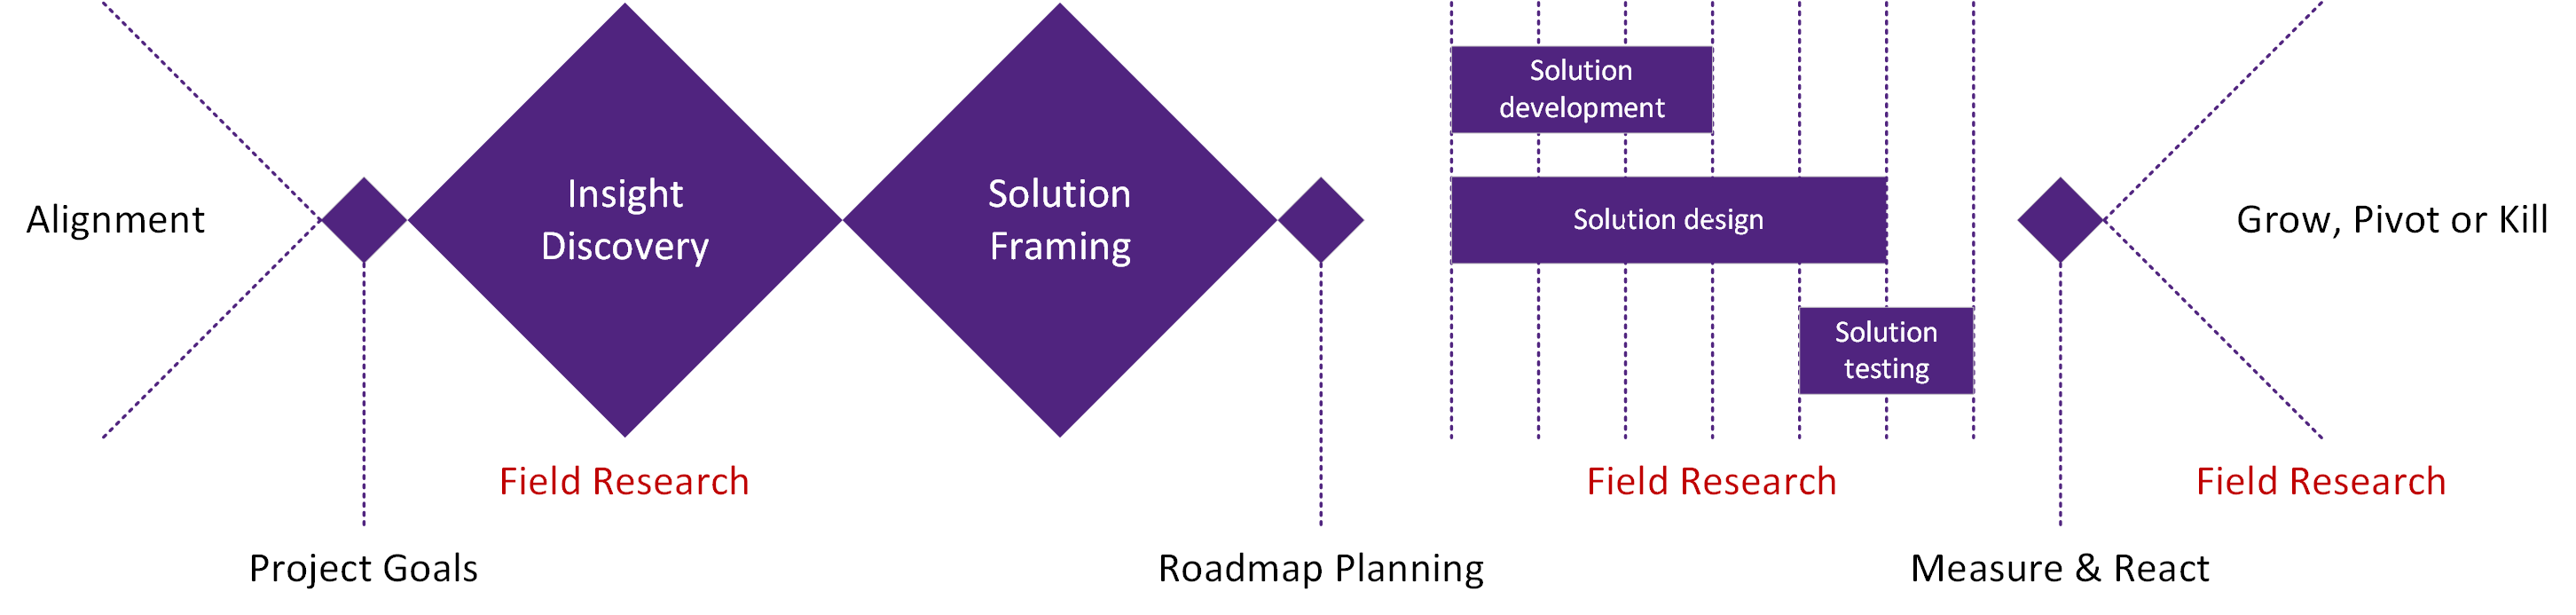
\includegraphics[width=16cm]{../../Images/DoubleDiamond.png}
  \caption{The double diamond model and shows how the discovery process embeds field research \parencite{OTH02}.}
  \label{fig:ddm}
\end{figure} 

Interesting pieces of information might surface during the field research. These pieces of information, ideally directly quoted from the source, are defined as \emph{insights} \parencite{OTH02}. An opportunity arises from a positive insight: it delights the stakeholder and motivates action. A challenge arises from a negative insight: it frustrates the stakeholder and potentially blocks the success. The product team frames a solution based on the insight. The solution goes back into the field research where a product team use new insights for further development, design, and testing. Once finished, there are three options: grow (continue), pivot (restart) or kill the project.

\paragraph{Goals and requirements} \label{gr}
Requirements prioritisation decides which requirement is most important in the context of an insight. Alternative solution selection decides the best way to address an insight. Defining what a solution exactly is and where it is coming from further supports building the common understanding.

We use the definition: \textit{'A goal is a prescriptive statement of intent the system should satisfy [...]'} \parencite{BK04} and define that a goal is equal to a solution. A software engineer needs a detailed view on a goal and slices the goal into multiple sub-goals or requirements: \textit{'A requirement is a goal under the responsibility of a single agent of the software-to-be'} \parencite{BK04}. As a result, a requirement achieves a (sub) goal. It adds customer value, even though it might not be able to address the primary goal directly. The relationship between a primary goal, potential sub-goals, and the related requirements is called a goal-model. The goal-model shows how higher-level goals are satisfied by lower-level goals (or requirements). Figure \ref{fig:gm} presents an example of a goal-model.

\begin{figure}[H]
\centering
  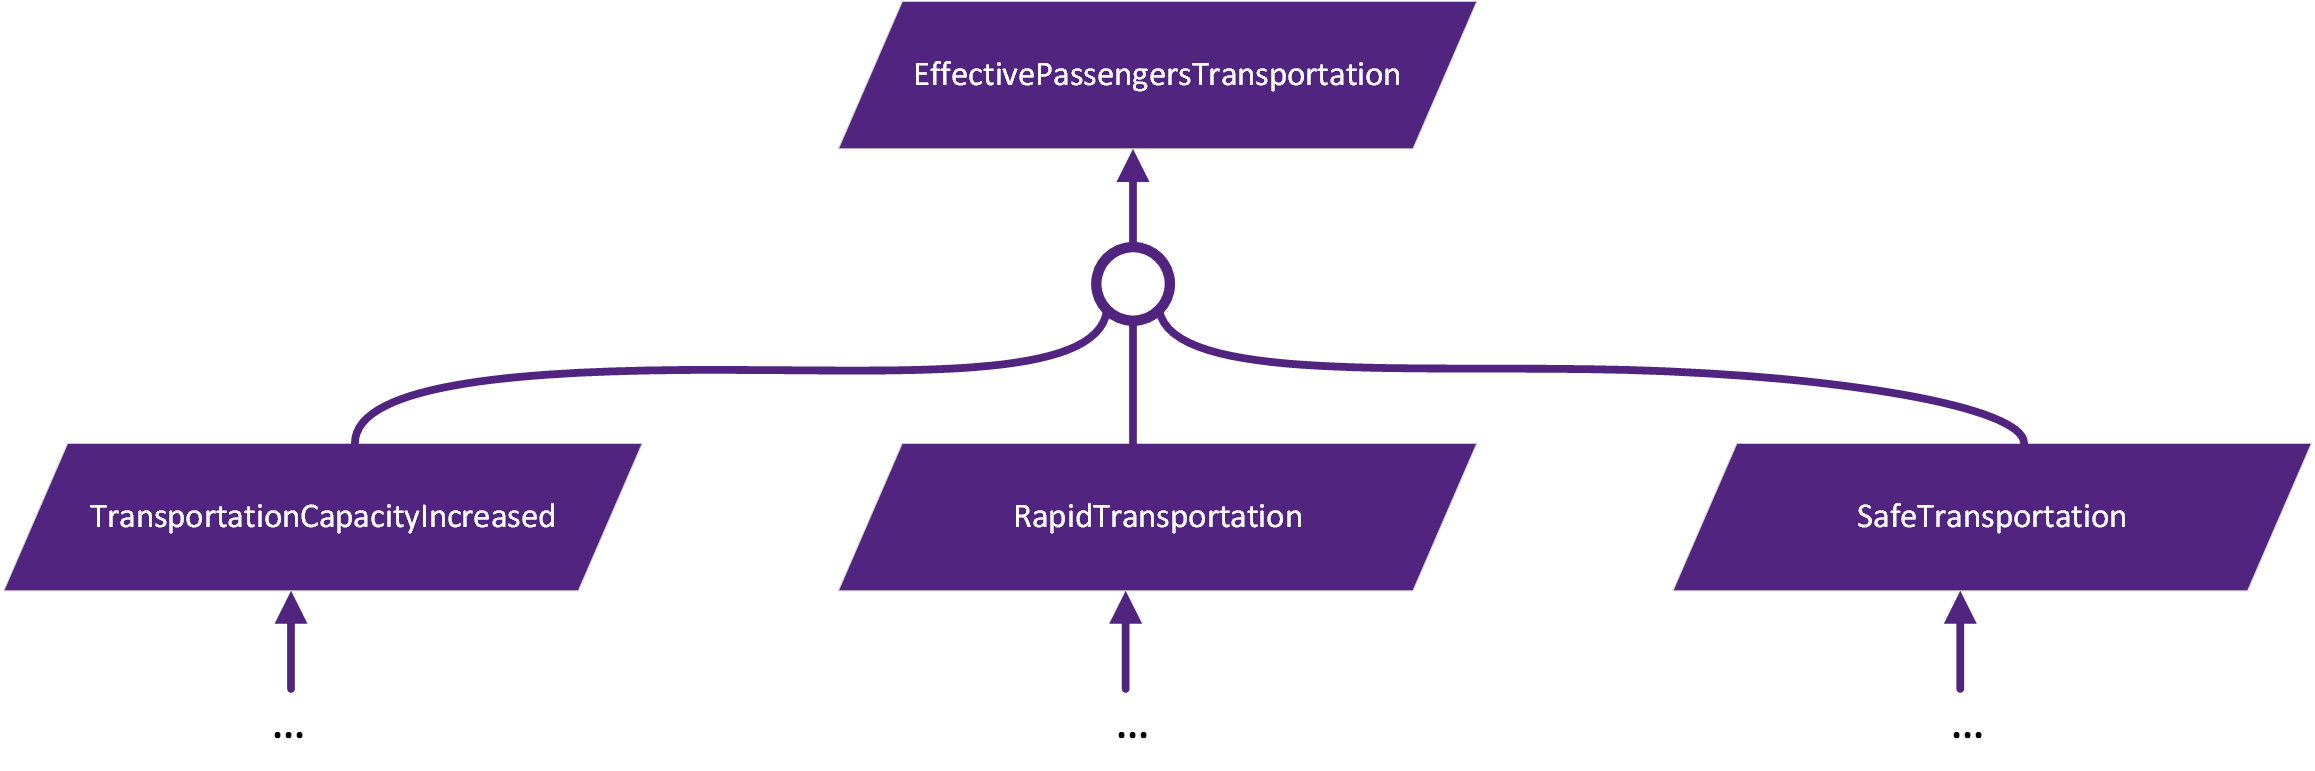
\includegraphics[width=15cm]{../../Images/GoalModel.png}
  \caption{Example of a goal-model showing the primary goal (effective passenger transportation) and its related sub-goals \parencite{BK04}.}
  \label{fig:gm}
\end{figure}

\subsubsection{Requirements prioritisation} \label{tf-val-rp}
Software is never finished: there is an endless number of requirements to improve software products or to increase its usefulness or to create a competitive advantage. Picking the right requirements can lead to great success while picking the wrong requirements can lead to utter failure \parencite{PM17}. The requirement prioritisation process focusses on a decision involving two requirements: which one is more important? 

\paragraph{An informal process that is driven by intuition} 
The requirements prioritisation process is informal and includes invisible decisions \parencite{PM20}. Continuously changing information requires that prioritisation is a continuous or iterative process. The software product manager needs to repeat this process regularly \parencite{PM22}.

The most popular technique for requirements prioritisation is the analytical hierarchical process, followed by the quality functional deployment, planning game, and binary search tree \parencite{PM29}. However, product managers hardly use these techniques, as most of them produce unreliable results or are very time-consuming. For example, the software product manager needs to manually update the prioritisation of the relevant requirements when a new requirement is introduced or deleted from the list \parencite{PM29}. 

\begin{quote}\itshape
'There is no time to analyse thousands of wishes[requirements]; much of the work is done intuitively.' \parencite{PM20}
\end{quote}

\paragraph{Criteria that influence the priority} \label{rpp_solution} 
A requirement starts with the stakeholder (typically a customer or user): an insight either motivates the stakeholder to take action (opportunity) or frustrates the stakeholder (challenge). The insight needs to contribute to achieving the product vision. Product managers should tightly couple the product vision to the value the product offers to the market \parencite{PM16}. The \emph{value} of the insight and the \emph{vision contribution} should influence the priority of the related requirements as well.

Depending on the environment, multiple stakeholders might recognise the same insight, which increases its value for the organisation. The \emph{reach} of the insight, therefore, should influence the priority of the related requirements.

A single requirement can rarely solve an insight on its own, and multiple goal-levels can be in between the insight and requirement \parencite{BK04}. The team implementing the requirement needs to define the \emph{contribution} level to the insight. At the same time, each requirement should address a small part of the insight independently. The \emph{contribution} of a requirement to each insight should influence the priority of the requirement.

From a business perspective, the product manager needs to balance the cost of developing a requirement with the business value the requirement brings \parencite{BK04}. The business value includes, for example, the costs of not implementing a requirement. The product manager should prefer requirements with high business value and a low cost over requirements with low business value and a high cost. The \emph{value} and \emph{cost} ratio should, therefore, influence the priority of a requirement.

The team implementing the requirement needs to be confident the requirement is achievable and that the requirement can address (a part of) the insight. Confidence does not only mitigate financial risks, but it also increases the efficiency of the team, and it will motivate them to implement the requirement in a way it will meet the stakeholders' expectations \parencite{PM23}. The \emph{confidence} should, therefore, influence the priority of a requirement.

\paragraph{Relative scale}
A relative scale is suitable to estimate the values of the proposed criteria \parencite{PM22}. However, a relative scale has a disadvantage as well. The scale changes when the software product manager introduces a new requirement or removes an existing requirement. This challenge can be mitigated by trying to fit requirements into a predefined scale.

\subsubsection{Alternative solution selection} \label{tf-val-as}
Each product (or product functionality) has a goal \parencite{SO03}. A goal can range from reducing the operational costs or increasing the scalability of the product. Traditional requirements engineering modelling techniques do not include the analysis of alternative solutions \parencite{SO12} that could cause the product team to select a premature solution. The outcome of this decision is a chosen solution for reaching a specific goal. Based on this decision, the team can start the implementation.

\paragraph{Selecting the best possible solution} 
An organisation starts a software project with an agreement on \emph{what} problem should be solved, \emph{why} the problem needs to be solved and \emph{who} should be involved in solving that specific problem \parencite{SO03}. For each problem, multiple (software) solutions are available. The complexity of each solution is partly defined by its functionality and by a set of non-functional requirements related to, for example, operational costs, performance, reliability, maintainability, portability, and robustness \parencite{SO06}. 

\begin{quote}\itshape
'Errors of omission or commission in laying down and taking properly into account such [non-functional] requirements are generally acknowledged to be among the most expensive and difficult to correct once the information system has been completed.' \parencite{SO06}
\end{quote}

\paragraph{Quantitative Reasoning} 
A solution describes the effect of the system-to-be on its surroundings. The product team defines the goal of the system-to-be and its composition, which might contain other (sub)goals or system requirements \parencite{SO03}. Out of the potential combinations of goals and requirements, the best solution needs to be selected. 

Product teams can use soft goals as evaluation criteria for selecting solutions among multiple alternatives \parencite{BK04}. A soft goal is a particular type of goal for which it is not possible to establish its reachability. It is possible to state a soft goal is more satisfied in alternative $a$ compared to alternative $b$. There are two options to evaluate alternative solutions using soft goals: qualitative reasoning and quantitative reasoning \parencite{BK04}. The disadvantage of qualitative reasoning is that the propagation rules have a high probability of generating an inconclusive outcome that does not make it suitable for this study. 

\begin{quote}\itshape
'The aim is to determine, for each alternative, a [...] degree of satisficing of the top-level soft-goals in the goal refinement graph; the option with the best degrees of satisficing is then selected.' \parencite{BK04}
\end{quote}

Qualitative reasoning assesses the positive or negative contribution of a solution to the soft goal: the product team needs to score each potential solution against the soft goal. A score $x$ means that the solution contributes to the soft goal for $x$\% \parencite{BK04}. Figure \ref{fig:sg} presents the goal \emph{optimal track usage}. Optimal track usage is essential for the busy rail network in, for example, Japan. The system-to-be needs to achieve this (soft) goal while taking safe transportation into account. There are two potential solutions for avoiding a train collision: avoiding trains to enter the same rail block and maintaining a worst-case stopping distance. Assuming the worst-case stopping distance is shorter than the entire rail block, this is the chosen solution. It allows maximising the rail block usage while avoiding train collisions.

\begin{figure}[H]
\centering
  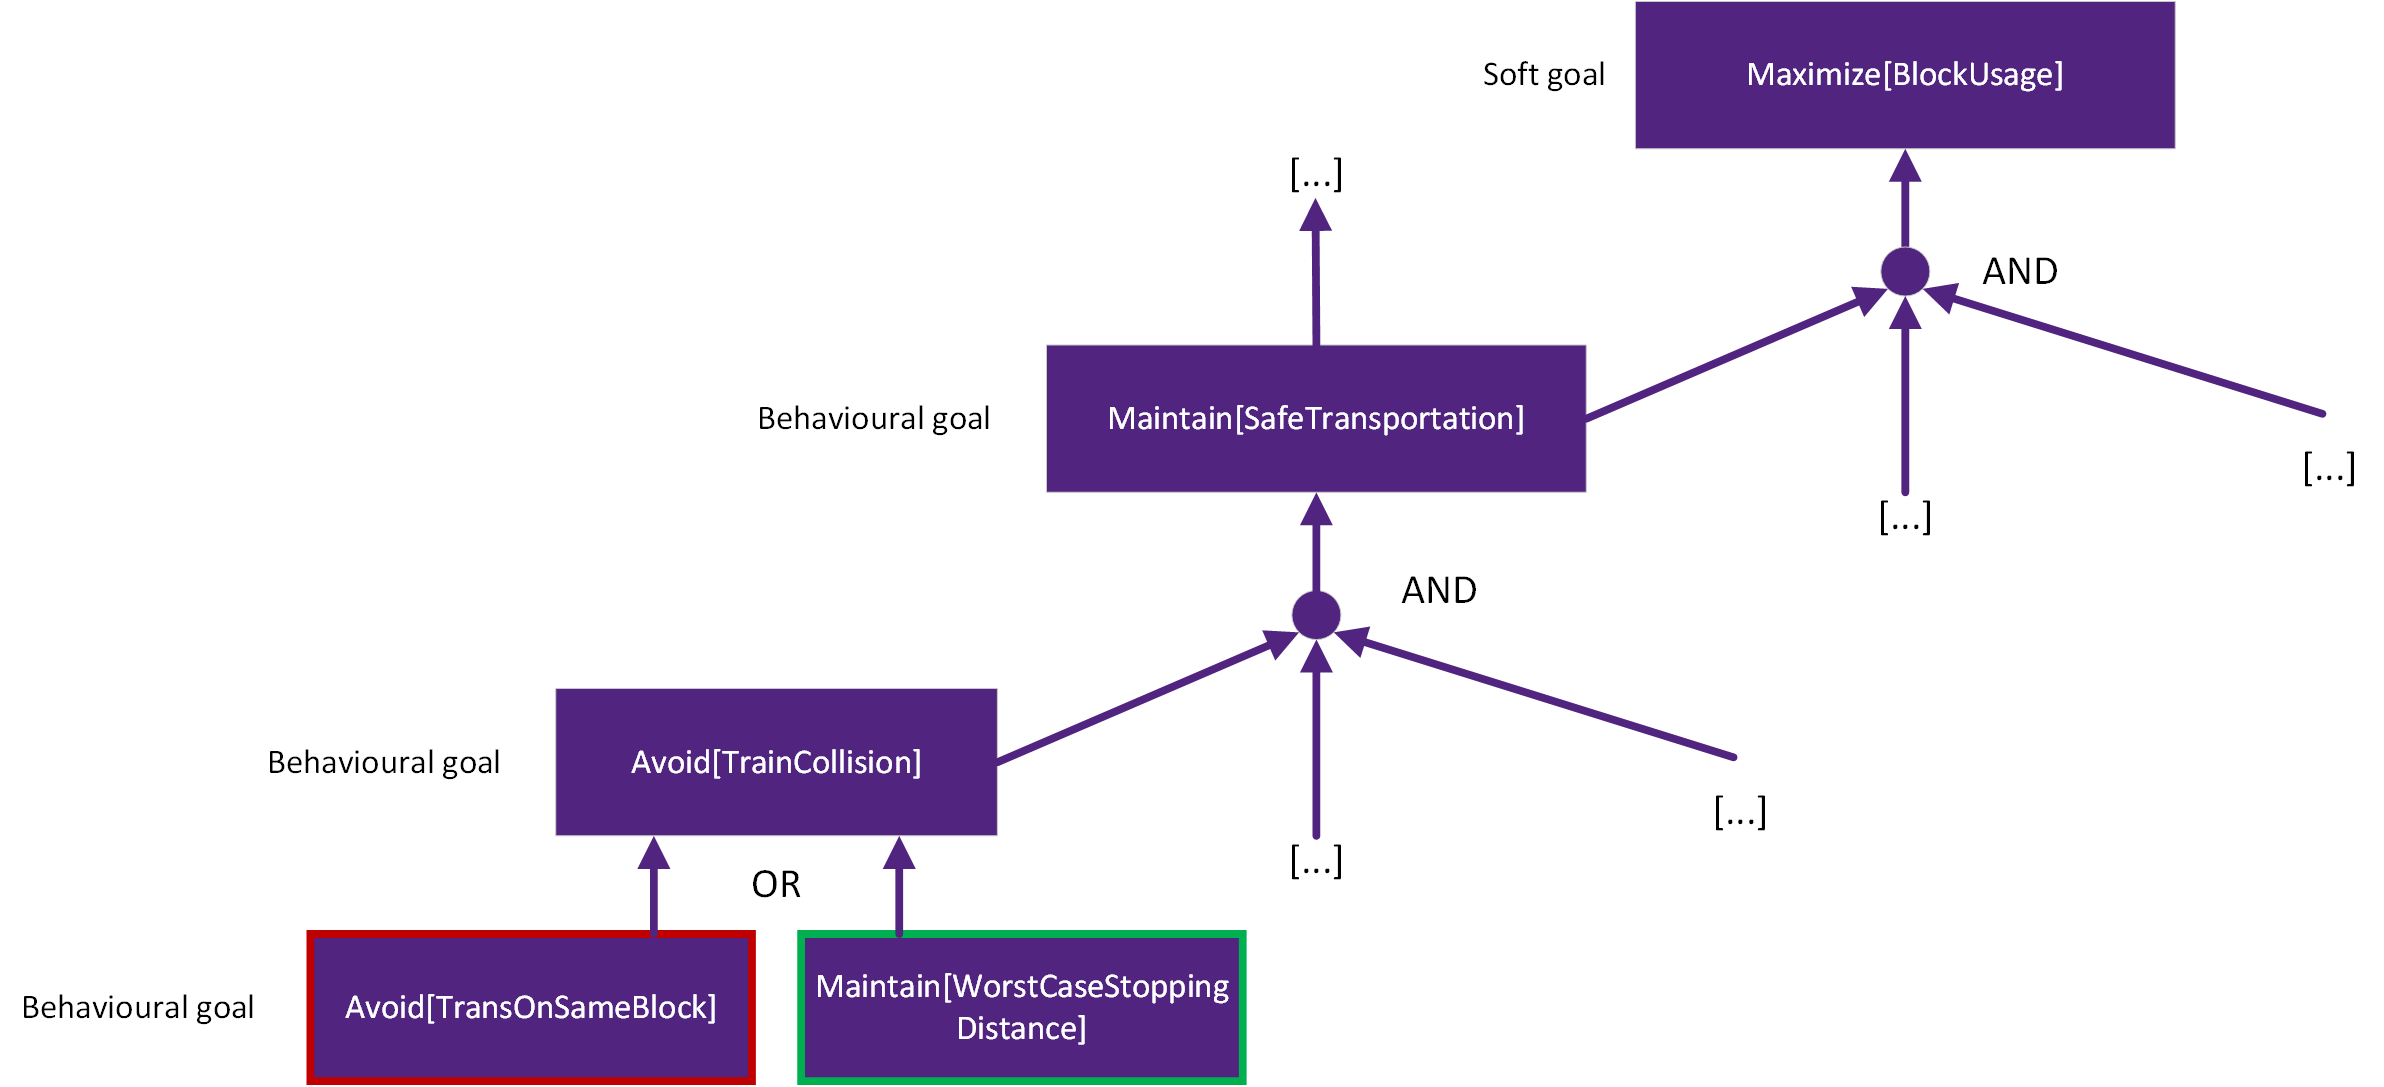
\includegraphics[width=17cm]{../../Images/SoftGoal.png}
  \caption{The selection of a solution for the efficient usage of a railway system based on higher-level soft goal \parencite{BK04}.}
  \label{fig:sg}
\end{figure}

We assign each soft goal with a weighted significance when the system-to-be needs to achieve multiple soft goals. \cite{BK04} proposes to use equation \ref{eq:totalScore} to calculate the total score that sums up the individual scores of the solutions and weighs them based on relative importance.

\begin{equation} \label{eq:totalScore}
totalScore(solution)=\sum_{soft\text{-}goal} (Score(solution,soft\text{-}goal) \times Weight(soft\text{-}goal)) 
\end{equation}

Equation \ref{eq:totalScore} calculates the value of the combined solution and soft goal by multiplying the weighted significance of a soft goal with the score of the solution. The sum of the values assigned to a solution determines the evaluation of the solution (equation \ref{eq:totalScore}). Table \ref{table:itass_example} shows an example where the equation prefers to maintain the $WorstCaseStoppingDistance$ over avoiding $TrainsOnSameBlock$ \parencite{BK04}.

\begin{table}[H]
\centering
\caption{Example of the usage of equation \ref{eq:totalScore} in which $Maintain[WorstCaseStoppingDistance]$ is preferred over $Avoid[TrainsOnSameBlock]$.}
\begin{tabular}{| p{4cm} | p{2cm} | p{4cm} | p{5cm} |}
\hline
\rowcolor{document}
\color{documentText}Soft-goal & \color{documentText} Significance weighting & \color{documentText}Maintain [WorstCaseStoppingDistance] & \color{documentText}Avoid [TrainsOnSameBlock] \\
\hline
Maximize[BlockUsage] & 0.50 & 0.90 & 0.30 \\
\hdashline
Soft goal 2 & 0.30 & 0.50 & 0.90 \\
\hdashline
Soft goal 3 & 0.10 & 0.80 & 0.30 \\
\hdashline
Soft goal 4 & 0.10 & 0.50 & 1.00 \\
\hline
Total & 1.00 & 0.73 & 0.55  \\
\hline
\end{tabular}
\label{table:itass_example}
\end{table}

% Summary of the theoretical framework.
\subsection{Conclusion} \label{tfconclusion}
Decision-makers use more than written or scientific sources to make their decisions. The values and experience the decision-maker and organisation bring influence the decision. A decision is always time-critical. There is a balance between elaborating on the available information to increase the maturity-level and accepting the current maturity-level of the available information and making the decision. The perfect decision does not exist. There is always some prematurity in the information decision-makers have access to and limited time to increase the maturity-level. 

\begin{center}
\large\color{document}{When decision-makers know the maturity-level, they can explicitly decide to spend more time to elaborate on the information or to make the decision based on the current maturity-level.} \\
\end{center}

The Semantic Web offers capabilities to validate if the information stored in an ontology is consistent, to classify information, and to detect missing information. We see an opportunity to bridge these capabilities to detect, for example, if specific information is reproducible or meeting a certain consensus-level. 

Design patterns exist in different flavours but have one thing in common: they solve a general problem. Generic ontology design patterns can generalize a data structure. We have not been able to find design patterns for other Semantic Web technologies, for example, SWRL rules or SHACL constraints. Information presentation design patterns do not seem to exist literally. However, we can extract information presentation patterns from existing scientific and commercial sources. 
\section{Methodology} \label{methodology}
This chapter describes how we use the theoretical framework to answer the research question. We share all the source files related to this study using a GitHub repository: \href{https://github.com/marioverhaeg/cs-thesis}{https://github.com/marioverhaeg/cs-thesis}.

\subsection{Research question} \label{meth_scope}
\subsubsection{Scope}
The results of this study should help decision-makers to move to evidence-based decision-making. This goal leads us to the main research question:
\begin{center}
\large\color{document}{\researchquestion} \\
\end{center}

We detect premature information using its completeness and reliability. We base the completeness of decision-relevant information on the availability of the required information and base the reliability of the decision-relevant information on the three metrics described in section \ref{tf_dmm} \nameref{tf_dmm}: reproducibility, consensus, and conflict. This decision meta-information allows us to calculate the information maturity-level. Section \ref{tf_dmm} \nameref{tf_dmm} also indicates that evidence-based decision-making depends on the quality of information. The information maturity-level measures the maturity, or quality, of information. Therefore, a higher information maturity-level contributes to evidence-based decision-making.

\paragraph{Ontology structure}
We use Semantic Web technologies to store the information that decision-makers use to justify their decisions. First, we need to know if we can create an ontology for evidence-based management. Next, we need to ensure that we can store the information completeness and reliability in this ontology and, based on the completeness and reliability, detect premature information. 

\begin{center}
\large\color{document}{\rqdsone} \\[0.3cm]
\large\color{document}{\rqdstwo} \\[0.3cm]
\large\color{document}{\rqdsthree} \\
\end{center}

\paragraph{Data presentation}
We transform the information completeness and reliability into the information maturity-level. Therefore, we need to define the information maturity-level explicitly. Once we know when a decision-maker is interested in the information maturity-level, we can find the right way to present the information maturity-level to the decision-maker. This presentation should make it easier for the decision-maker to understand the information maturity-level and decide if the decision-relevant information is mature enough to make the decision.

\begin{center}
\large\color{document}{\rqvisone} \\[0.3cm]
\large\color{document}{\rqvistwo} \\[0.3cm]
\large\color{document}{\rqvisthree} \\
\end{center}

\subsubsection{Out of scope}
The scope of this study is limited to verify if it is possible to detect premature information and to find the right way to present the information maturity-level to a decision-maker. The implementation in a production environment requires a different focus and scope. Premature information will stay premature until the decision-maker extends the ontology with new information or adjusts existing information. Extending the ontology with new information or adjusting existing information is not in the scope of this study. We also exclude an analysis of the scalability and performance of our proposals.

\subsection{Scientific approach} \label{meth_sa}
We answer the research questions using a case-study based on the reasoning and structure proposed by \cite{THE08}. The way we phrased the research question and the related sub-questions indicates a case study would be the most suitable method to answer these questions \parencite{BK06}. Figure \ref{fig:ds1} presents our conceptual approach. There is a natural iteration between the main contribution and the validation. We need to adjust a pattern if we question its suitability to solve the specified problem in the given context. When we adjust a pattern, the validation of the pattern in other contexts might require adjustments as well.

\begin{figure}[H]
\centering
  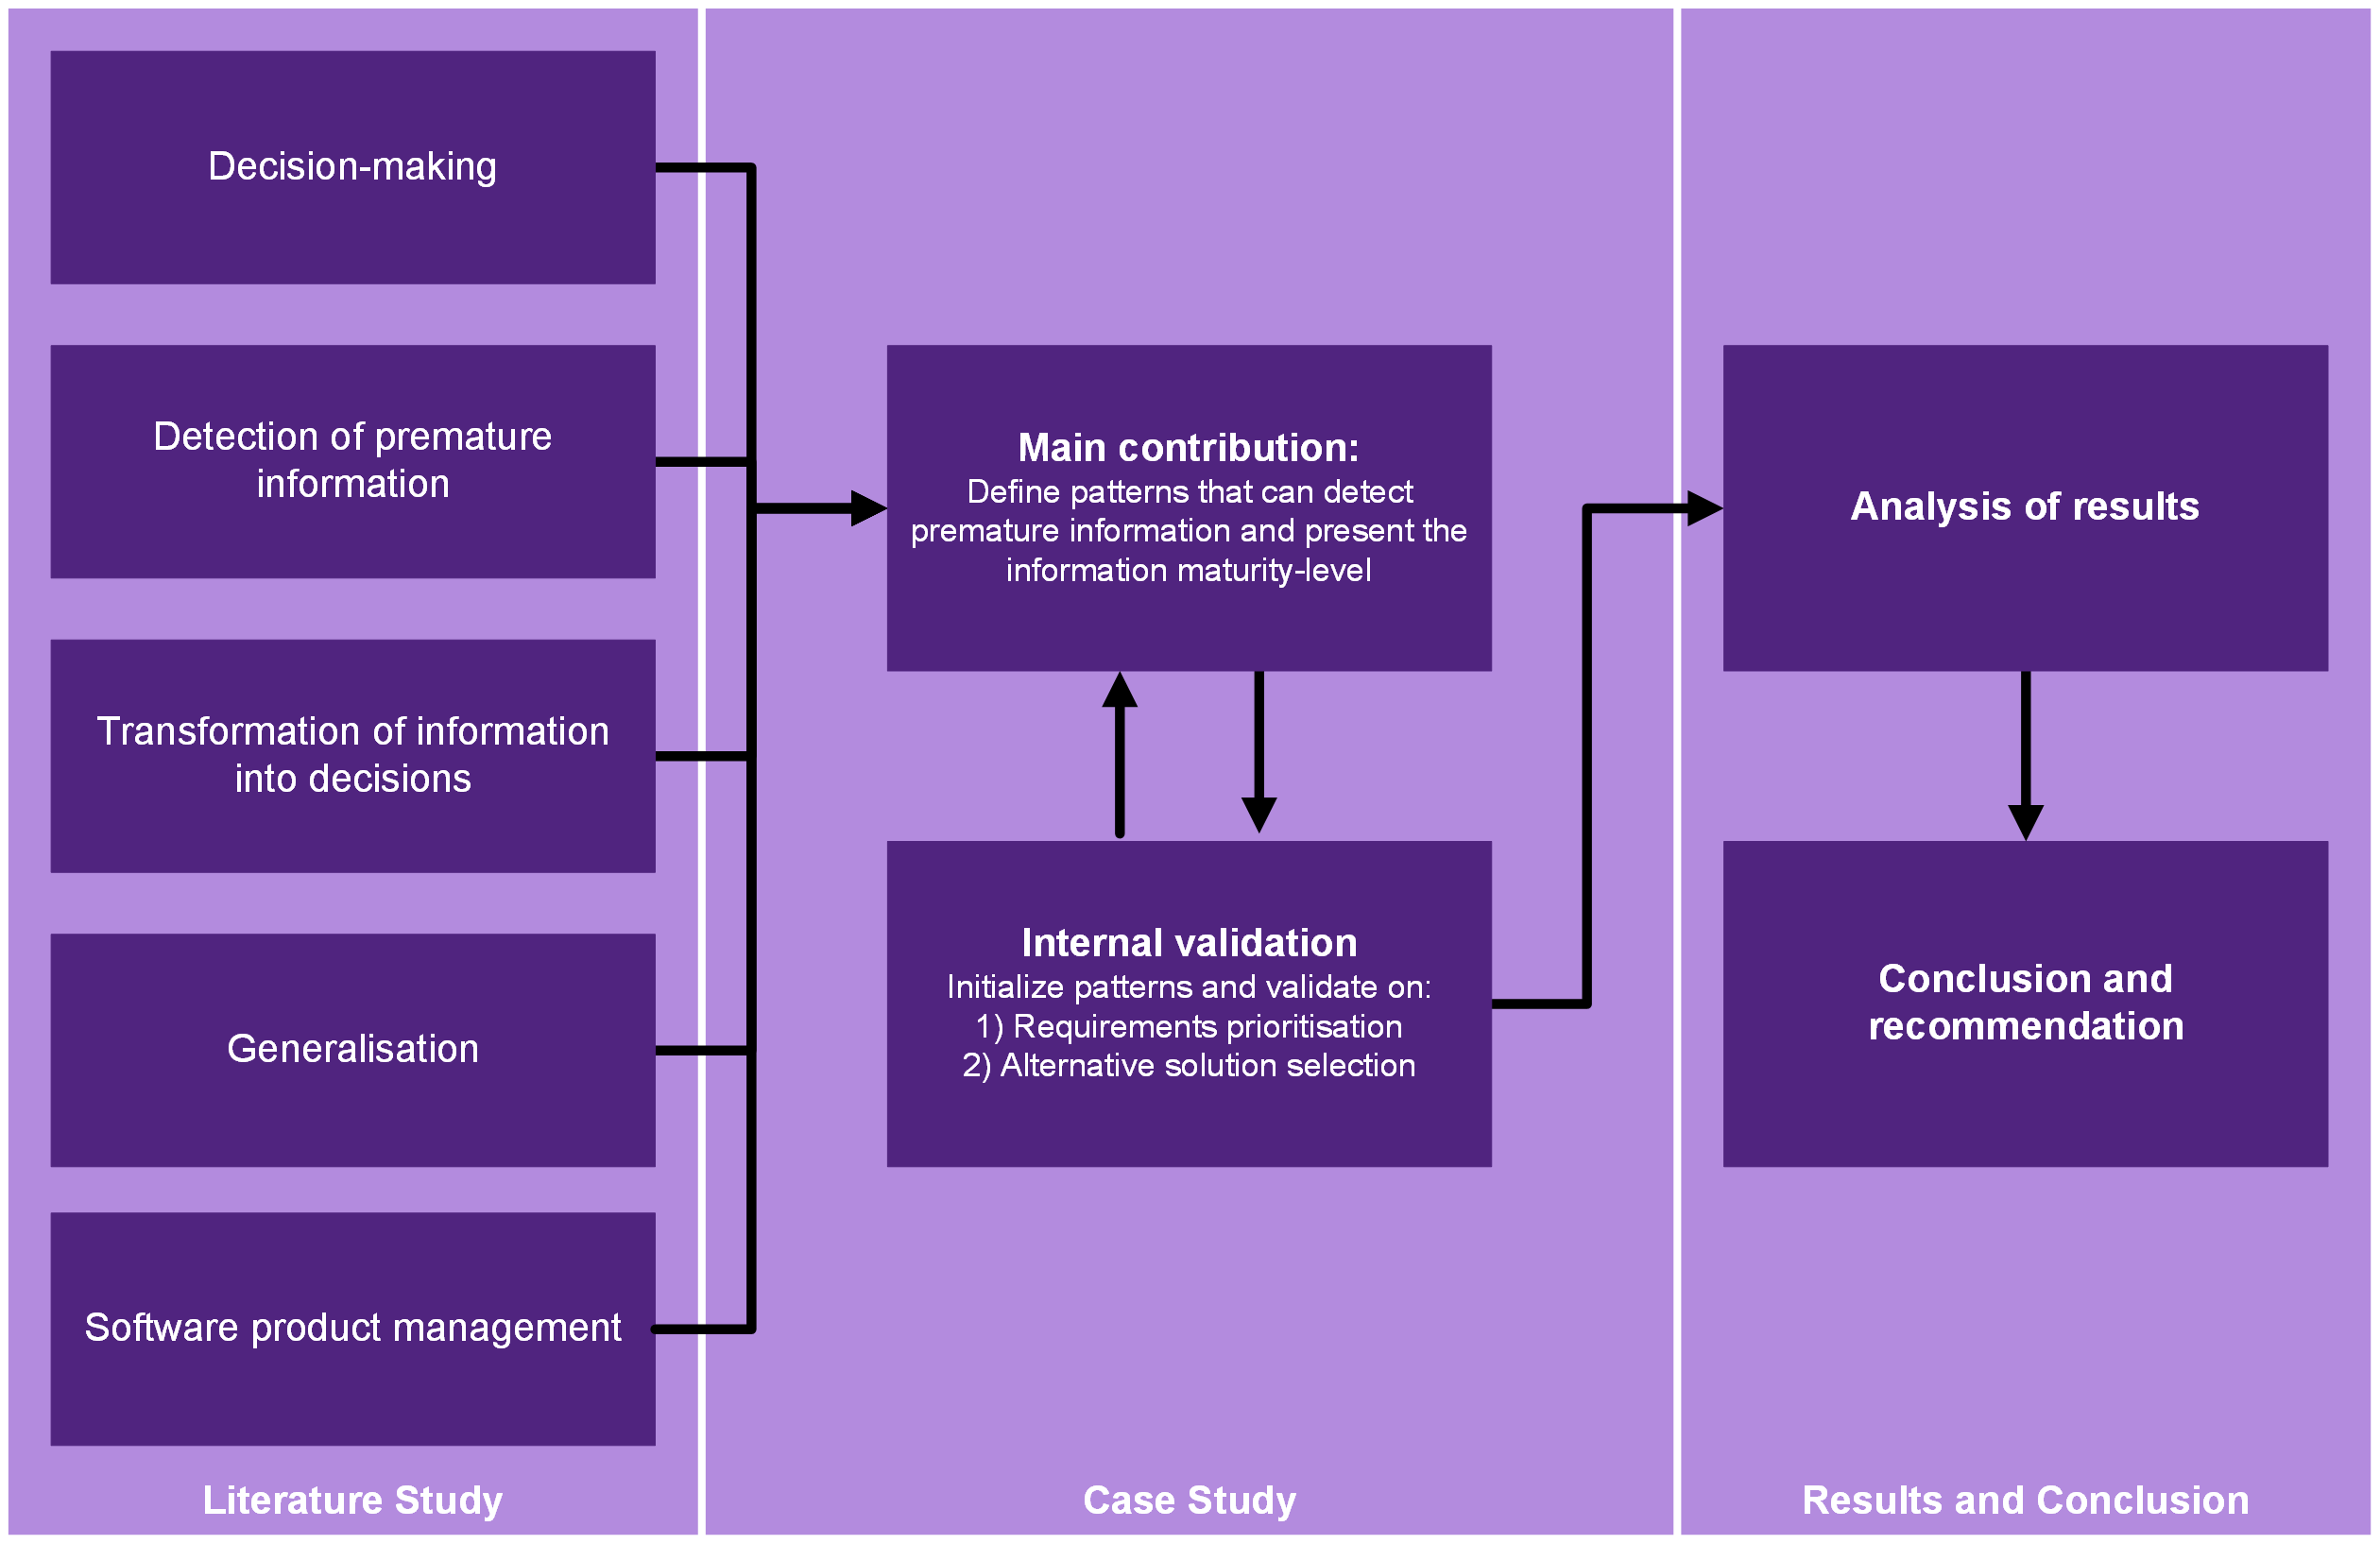
\includegraphics[width=16cm]{../../Images/03_Methodology/03_METH_Phases.png}
  \caption{The conceptual approach of this study, including the literature study, case study, and finalization phases. We re-use a structure proposed by \cite{THE08}.}
  \label{fig:ds1}
\end{figure}

A case study confirms the proposed concept works in a specific case. A pattern solves a general problem and should, therefore, be generally applicable. We validate the pattern on two scenarios to increase our confidence that the pattern is generally applicable. The first scenario validates the pattern and includes an extensive description of its reasoning and background. We reduce the level of detail in the second scenario to prevent repetition. We indicate when we leave out details and will refer to the approach we use in the first scenario. 

\subsection{Activities} \label{activities}
Table \ref{table:Tools} presents an overview of the tools described in this section\footnote{Prot\'eg\'e 5.5.0 uses rdflib 3.0.0. Rdflib 3.0.0 has an issue that prevents \emph{SPARQL COUNT DISTINCT} from working correctly (\href{https://github.com/RDFLib/rdflib/issues/404}{issue 404}). This issue is fixed in rdflib 5.0.0, but this version is not merged into Prot\'eg\'e yet. We ran into this issue on several occasions and worked around it by removing the COUNT and looking at the number of results of the SPARQL query.}.

\begin{table}[!htbp]
\centering
\caption{An overview of the tools used for this study.}
\begin{tabular}{| p{2cm} | p{1,5cm} | p{13,5cm} |}
\hline
\rowcolor{document}
\color{documentText}Name & \color{documentText}Version & \color{documentText}Description \\
\hline
\href{https://protege.stanford.edu/}{Prot\'eg\'e} & 5.5.0 & We use Prot\'eg\'e to create the base of the generic ontology design pattern, instantiating them manually and hosting the SHACL4P plugin. \\
\hdashline
\href{https://github.com/fekaputra/shacl-plugin}{SHACL4P} & 1.0.0 & We use SHACL4P for syntax checking and validating the constraints on instantiated generic ontology design patterns. \\
\hdashline
\href{https://github.com/spechub/Hets/tree/1899_gdol_parser}{HETS} & n/a & We use a branch of HETS ($1899\_gdol\_parser$) that adds support for Generic DOL, which is an extension of DOL. \\
\hline
\end{tabular}
\label{table:Tools}
\end{table}

\subsubsection{Ontology design patterns} \label{gen_meth}
We use generic ontology design patterns, described in section \ref{tf_odp} \nameref{tf_odp}, to define our ontologies formally. We use the open-source tool Prot\'eg\'e (the most widely used software for building and maintaining ontologies \parencite{ME08}) to create the base of the generic ontology design patterns and instantiate them manually. Additionally, we use HETS (the heterogeneous toolset) to validate the syntax of the generic ontology design patterns. At this moment it is not possible to use HETS to instantiate generic ontology design patterns into new ontologies or merge them into existing ontologies. We enter the ontologies into Prot\'eg\'e manually. 

\subsubsection{Detecting completeness and reliability}
We define a multi-layered model using Semantic Web technologies. This model can detect the completeness, consensus, conflict, and reproducibility of information or evidence. 

The first layer infers new information. Inferring information reduces the complexity of the constraints. We introduce a hierarchy of object properties and classes. When we connect two individuals using an object property in a hierarchy, the reasoner infers that the two individuals are connected by the parent of the used object property as well. Figure \ref{fig:ifop} presents an example of object property inferencing. In this case, we can define a single constraint for the abstraction layer, instead of defining multiple constraints that need to handle each case individually. Additionally, we further reduce the constraint complexity using the characteristics of an object property to infer chains of information and reduce the existing chains back into a single object property. Last, the reasoner infers class membership from the domain and range of an object property. Class membership ensures that the constraints are applied to the right information.

\begin{figure}[H]
\centering
  
\includegraphics[width=8cm]{../../Images/03_Methodology/03_Inferring_Object_Properties.png}
  \caption{This example shows that the reasoner infers the object property $has\_information$ when the individual hosts the object property $has\_information\_insight$.}
  \label{fig:ifop}
\end{figure}

The second layer ensures the structural consistency of the ontology by defining that specific classes or object properties are disjoint. This definition makes the second layer especially useful to detect mistakes in the configuration of the inferencing rules.

The third layer validates the completeness and reliability of decision-relevant information:
\begin{enumerate}
\item We base the completeness on the existence of specific data- and object properties
\item Reproducibility equals the number of evidence sources used for decision-relevant information.
\item The consensus is equal to the number of agreements between different evidence sources.
\item The conflict is equal to the number of disagreements between different evidence sources.
\end{enumerate}

The decision design pattern defines Semantic Web constraints to detect incomplete information, the number of consensus and conflicts, and the number of evidence sources. We calculate the information maturity-level based on the number of violated constraints and the maximum number of constraints.

The Semantic Web provides two mechanisms to detect a violation of constraints: SPIN (SPARQL Rules) and SHACL. Compared to SHACL, SPIN never became a formal W3C standard, and the industry recognises SHACL as the successor of SPIN:
\begin{quote}\itshape
'SHACL supersedes SPIN in almost every respect. [...] Most importantly, SHACL is an official W3C Recommendation that makes it far more likely that other vendors will support it.' \parencite{WEB14}
\end{quote}

We select SHACL to detect the violation of constraints.

We use the Prot\'eg\'e plugin SHACL4P \parencite{SM25} to validate the SHACL shapes. SHACL4P allows us to define constraints and validates the ontology against those constraints. Figure \ref{fig:shacl-output} presents an example of the output of SHACL4P. 

\begin{figure}[H]
\centering
  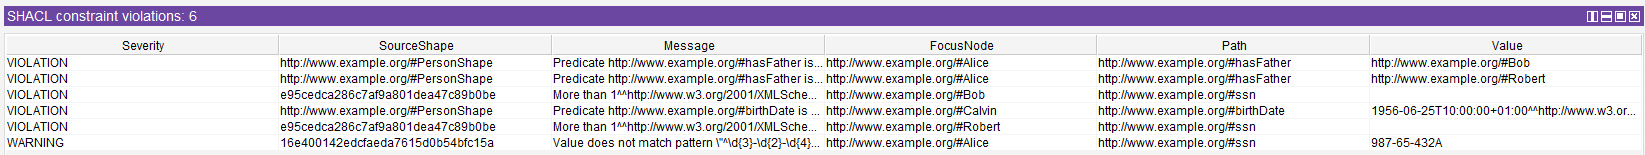
\includegraphics[width=17cm]{../../Images/SHACL4P_Example.png}
  \caption{An example of SHACL4P output showing constraint violations in Prot\'eg\'e.}
  \label{fig:shacl-output}
\end{figure}

\subsubsection{Constraint design patterns}
We cannot find an explicit definition of constraint design patterns. Therefore, we define the constraints in a way they are re-usable. We add parameters to the constraints when we need those constraints in the context of the ontology design patterns. When we use parameters, we need to instantiate the constraints manually. 

\subsubsection{Presentation design patterns} \label{meth_presentation}
We need to present the information maturity-level to the decision-maker. First, we extract information from the ontology to provide input to the functions that calculate the information maturity-level. Second, we select the right information presentation pattern based on the characteristics of the decision. We present the information maturity-level of the information using the selected pattern. 

We build mock-ups for the data presentation pattern using generic tools, for example, Microsoft PowerPoint.  

\subsection{Validation} \label{meth-validation}
We split the validation into reproducibility (how can the results of the study be reproduced?), internal validity (how can the results of the study be validated?), and external validity (how can de results of the study be applied to other cases?).

\subsubsection{Reproducibility}
We ensure the reproducibility of this study using scientific literature, documented interpretation of the literature, and where applicable, documented decisions. We use, when possible, open-source tools and use our GitHub repository (\href{https://github.com/marioverhaeg/cs-thesis}{https://github.com/marioverhaeg/cs-thesis}) to store the generic ontology design patterns, ontologies, constraints, and queries that we present in this document. Additionally, we also store the source of this document in the GitHub repository.

\subsubsection{Internal validity}
The goal of the decision design pattern is to motivate decision-makers to move from intuition-based decision-making to evidence-based decision-making by detecting premature information and presenting the information maturity-level. We also want domain experts to re-use the decision design pattern when they want their decision-makers to move from intuition-based decision-making to evidence-based decision-making. 

The internal validity addresses the validation of the research question based on the two scenarios described in section \ref{tf-val-rp} \nameref{tf-val-rp} and \ref{tf-val-as} \nameref{tf-val-as} of the theoretical framework:
\begin{enumerate}
\item \nameref{val-rp}
\item \nameref{val-as}
\end{enumerate}

\subsubsection{External validity}
The external validity addresses the validation of the research question based on the same problem in a different domain. This study focuses on a single domain (software product management). Therefore, external validation is outside of the scope of this study. We present the results of the study in a way it allows them to be applied to other domains as well.

\subsubsection{Sample data}
The goal of the sample data is to validate if the ontology design patterns we create are suitable to detect premature information and present the information maturity-level in requirements prioritisation and alternative solution selection. Unfortunately, it proved difficult to find sample data for requirements prioritisation and alternative solution selection. Therefore, we create sample data ourselves. We define multiple test scenarios. Each test scenario has its dedicated sample data and describes how this sample data contributes to the results of the scenario. 

Creating sample data also carries a risk: we might miss validating scenarios for which we have not created sample data. We try to mitigate this risk by separating the sample data for each test case and by creating small differences in the sample data we use for different test cases.

% Results
\section{Contribution} \label{contribution}
We propose the \emph{decision design pattern} to detect premature information and present the information maturity-level to a decision-maker. 

\begin{center}
\large\color{document}{The decision design pattern detects incomplete and unreliable information and presents the information maturity-level to a decision-maker.}
\end{center}

We define the reliability of decision-relevant information, described in section \ref{tf_dmm} \nameref{tf_dmm}, using the reproducibility of information, the consensus of evidence, and the conflict of evidence. 

The decision-maker can decide to review the information maturity-level at any moment in time. Some decisions have deadlines, are essential, and potentially have a high impact on an organisation. Decision-makers do not make decisions with a high impact overnight, and they take their time to gather information and understand the exact impact of their decision. The information maturity-level should evolve while the decision-maker adds and changes information and the decision deadline comes closer. This way, the decision-maker uses the transparency of the information maturity-level to increase the completeness and reliability of the decision-relevant information.

\subsection{Decision design pattern}
We bridge the technological knowledge management strategy, described in section \ref{tf-val-rp} \nameref{tf-val-rp}, to the decision design pattern. The evidence-based management pattern stores the knowledge criteria that the decision-makers require to make the decision. The decision ontology pattern uses generic ontology design patterns to define a data structure on top of the evidence-based management pattern. We add the decision presentation pattern to present the information maturity-level. Figure \ref{fig:contribution_architecture} presents the decision design pattern. We encapsulate the completeness, reproducibility, consensus, and conflict patterns into the decision ontology pattern to cover overlap in these patterns and instantiate them in a way they can function side by side.

\begin{figure}[H]
\centering
  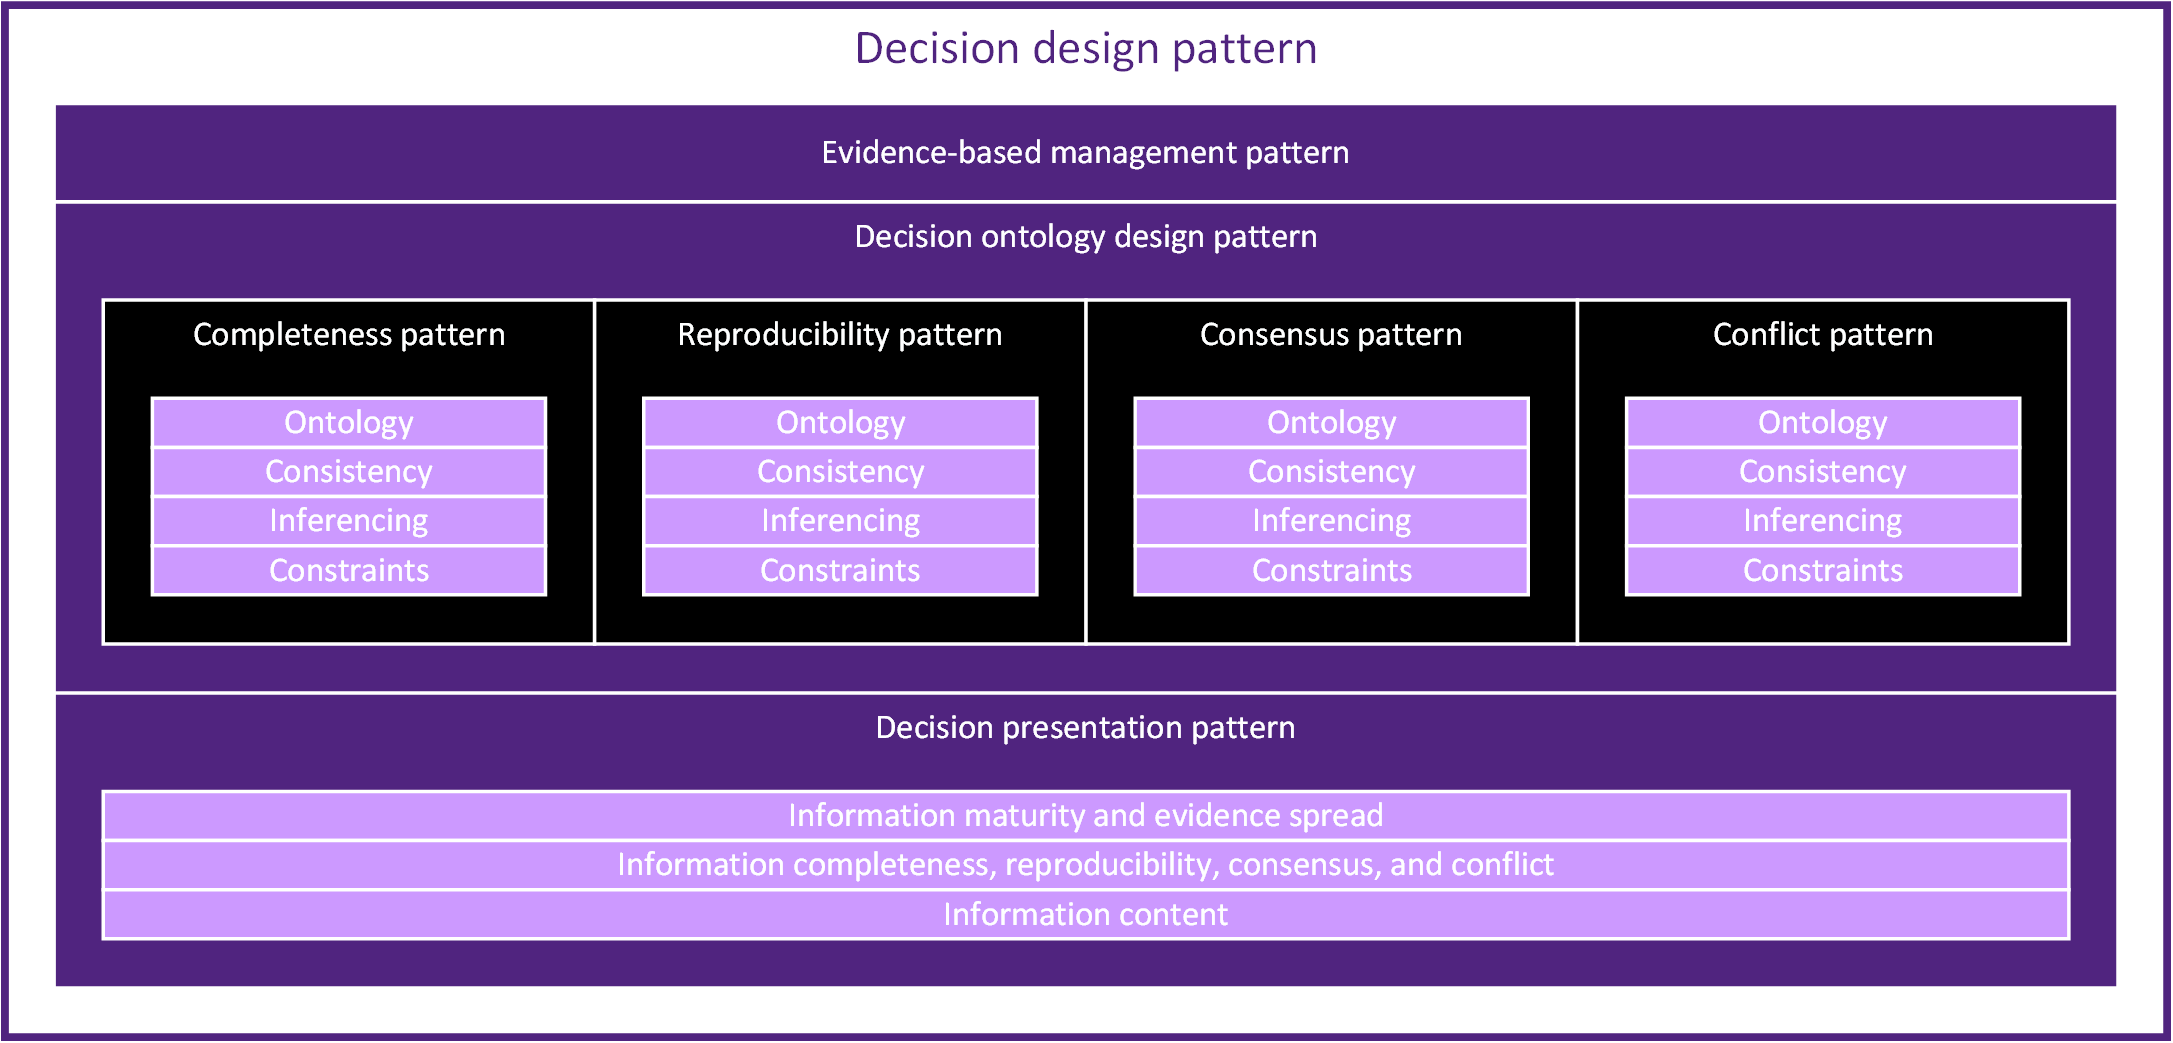
\includegraphics[width=17cm]{../../Images/04_Contribution/Pattern_Architecture.png}
  \caption{An overview of the decision design pattern that detects premature information and presents the information maturity-level. We encapsulate the completeness, reproducibility, consensus, and conflict patterns into the decision ontology design pattern.}
  \label{fig:contribution_architecture}
\end{figure}

We base the information maturity-level on the completeness and reliability of the information. The completeness pattern ensures that the information that a decision-maker needs to make a decision is available. The information needs to be reproducible by relating it to specific evidence sources. Additionally, we use two other patterns to measure the reliability of evidence: the conflict-level, and the consensus-level. The consolidation layer calculates the decision specific information maturity-level. 

With this approach, we deviate slightly from the categories we describe in section \ref{tf_dmm} \nameref{tf_dmm}. We remove the information collection methodology from the scope. We capture a part of the information collection methodology in the evidence types. For example, decision-makers typically gather evidence that we classify as $Contextual\_Circumstance$ using observation while they can only gather $Stakeholder\_Evidence$ by some form of interaction with the stakeholders. 

The decision-maker gets a general understanding of the information completeness and reliability using the information maturity-level and evidence-spread dashboard. We present the completeness, reproducibility, consensus, and conflict maturity-levels when the decision-maker wants to understand the information maturity-level in more details. Last, we present the completeness, reproducibility, consensus, and conflict levels per individual, including the violations. The decision-maker can use these details to increase the information maturity-level of a decision or optimise the evidence-spread. 

We present multiple ontology design patterns in the next sections of this chapter. Each pattern introduces a challenge and the ontology that addresses this challenge. The included generic ontology design pattern enables domain experts to re-use the ontology in different scenarios. Additionally, we describe how we guard the consistency of the ontology, and we describe the inferred information. We present the constraints that detect premature information in the last paragraph. Last, we introduce the main challenge of the decision presentation pattern and describe how we present the information maturity-levels to the decision-maker.

Only the combination of the patterns we describe in this chapter can address the challenge captured by the research question. Therefore, we focus our validation on the combination of patterns in a specific scenario. Section \ref{validation} \nameref{validation} presents the scenario-based validation that combines the patterns into a solution that addresses the challenge of the research question.

\subsection{Evidence-based management pattern} \label{odp_ebm}
% Subsection structure:
% Problem: what is the generalized problem?
% 	Motivation: why is this problem scientifically important and/or interesting?
% Solution: conceptual description of solution, including formal definition of GODP and SHACL constraints.
% 	Illustration: images of GODP structure.
% 	(Statistical)Analysis: how does the solution solve the problem?
% 	Evaluation: are the results significant? What is the impact?
\subsubsection{An evidence-based management structure}
Decision-makers need guidance to make decisions based on reliable information \parencite{DM07}. The evidence-based management pattern provides a structure to store evidence that decision-makers can use as a source for decision-relevant information. The pattern serves as a base for other patterns that validate the information completeness and reliability.

\begin{center}
\large\color{document}{The evidence-based management pattern supports the information completeness and reliability validation patterns by providing an evidence-based management structure.}
\end{center}

\subsubsection{Ontology}
We describe four evidence types in section \ref{tf_dmm} \nameref{tf_dmm}: practitioner expertise and judgement, evaluated external evidence, stakeholder preferences/values, and local context (organisational actors, circumstances). We add the evidence classes $Stakeholder\_Experience$ and $Stakeholder\_Values$ as subclasses of $Stakeholder\_Evidence$. We add $Stakeholder\_Evidence$ as a subclass to $Evidence$ itself. These evidence classes slightly deviate from their original definition. We rename \emph{practitioner} experience to \emph{stakeholder} experience for two reasons:
\begin{enumerate}
\item Practitioners are, generally spoken, a subset of stakeholders: practitioners are also considered stakeholders.
\item The previous definition excluded stakeholder experience and practitioner values as evidence: if stakeholder values are considered evidence, practitioner values should also be considered evidence. This reasoning is also valid for the experience. If we consider practitioner experience as evidence, we should consider stakeholder experience as well. 
\end{enumerate}
We add $Contextual\_Circumstances$ and $Evaluated\_External\_Evidence$ as subclasses of $Evidence$. The reasoner ensures the consistency of the ontology by defining the different evidence classes are disjoint. Figure \ref{fig:classification} presents the structure of the pattern.

\begin{figure}[hbpt]
\centering
  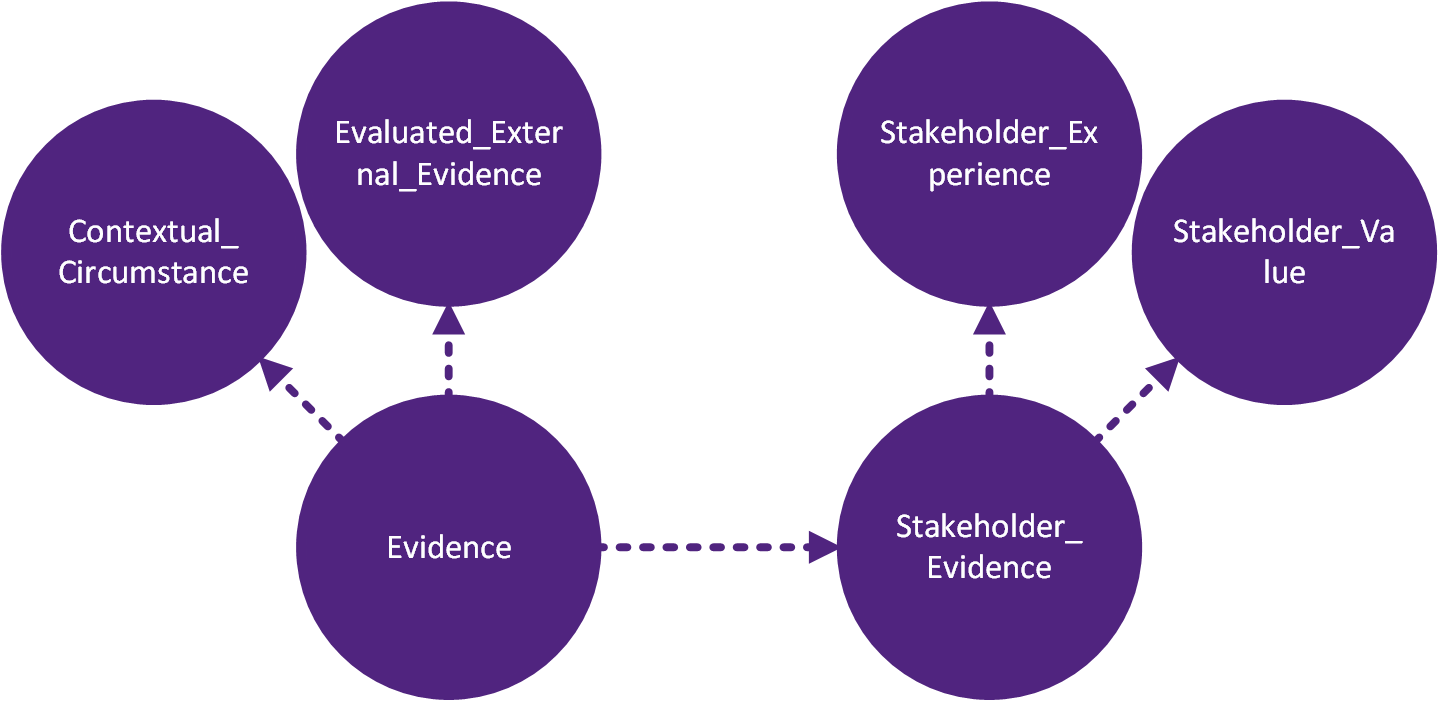
\includegraphics[width=9cm]{../../Images/04_Contribution/04_EBM_Classification.png}
  \caption{An overview of the evidence-based management ontology. $Stakeholder\_Experience$ and $Stakeholder\_Values$ as subclasses of $Stakeholder\_Evidence$. We add $Stakeholder\_Evidence$ as a subclass to $Evidence$ itself. Code sample \ref{GODP_EBM} presents the GDOL code that instantiates this ontology.}
  \label{fig:classification}
\end{figure} 

We create these classes for two purposes. First, the evidence spread determines the reproducibility of the evidence. The decision-maker can decide to gather additional evidence to increase the reproducibility of the decision-relevant information if, for example, the decision-relevant information is only based on $Stakeholder\_Experience$. Second, we extract $Contextual\_Circumstances$ from a written context or observation while we extract $Evaluated\_External\_Evidence$ from other written documents. We can reproduce this evidence based on its source. For $Stakeholder\_Evidence$, we need to know the stakeholder to reproduce it. Different evidence types have different behaviour and, therefore, need different classes.

\paragraph{Consistency}
We guard the consistency of the ontology using $DisjointClasses$. $Stakeholder\_Experience$ is logically different from $Stakeholder\_Value$. An individual cannot be $Stakeholder\_Evidence$, $Contextual\_Circumstance$, or $Evaluated\_External\_Evidence$ at the same time due to the difference in definition. When the reasoner classifies an individual as two disjoint classes, it will throw an inconsistency error and cannot continue reasoning. Figure \ref{fig:consistency_ebm} presents an example of an inconsistency error in Prot\'eg\'e. Code sample \ref{GODP_EBM} presents the implementation of the $DisjointClasses$.

\begin{figure}[H]
\centering
  
\includegraphics[width=17cm]{../../Images/04_Contribution/Consistency.png}
  \caption{An inconsistent ontology structure that a reasoner detects in Prot\'eg\'e. In this case, the individual $Contextual\_Circumstance\_SC0$ belongs to the classes $Contextual\_Circumstance$ and $Evaluated\_External\_Evidence$. $Contextual\_Circumstance\_SC0$ and $Evaluated\_External\_Evidence$ are disjoint classes. The reasoner does not accept that $Contextual\_Circumstance\_SC0$ belongs to both of these classes.}
  \label{fig:consistency_ebm}
\end{figure}

\paragraph{Inferencing}
The evidence-based management pattern uses a simple structure of classes and does not use inferencing to increase the amount of information in the ontology. 

\paragraph{Generic Ontology Design Pattern}
Code sample \ref{GODP_EBM} presents the generic ontology design pattern of the evidence-based management pattern using GDOL. We instantiate the evidence-based management pattern once per ontology it needs to extend. The evidence-based management pattern does not require parameters; therefore, we instantiate an $ontology$ instead of a $pattern$.

\begin{lstlisting}[float,language=GDOL,caption={The GDOL code that instantiates the generic ontology design pattern for evidence-based management. The instantiation includes the instantiation of the classes as well as the characteristics of those classes. Figure \ref{fig:classification} presents the structure of the pattern. },label={GODP_EBM}][H]
ontology EBM =
 Class: Evidence
 Class: Stakeholder
 Class: Stakeholder_Evidence SubClassOf: Evidence 
 Class: Stakeholder_Experience SubClassOf: Stakeholder_Evidence 
 Class: Stakeholder_Value SubClassOf: Stakeholder_Evidence 
 Class: Contextual_Circumstance SubClassOf: Evidence 
 Class: Evaluated_External_Evidence SubClassOf: Evidence 
 DisjointClasses: Stakeholder_Evidence, Contextual_Circumstance, Evaluated_External_Evidence	
 DisjointClasses: Stakeholder_Experience, Stakeholder_Value
\end{lstlisting}

\paragraph{Constraints}
It is possible to define constraints based on the stake of a specific evidence type. For example, the $Evaluated\_External\_Evidence$ should represent 20\% of the evidence related to a specific decision. However, these constraints would be very context-sensitive. We leave it up to the decision-maker to evaluate the mix of evidence-types manually on a case-by-case basis. Alternatively, the domain expert can manually add constraints based on the preference of the organisation implementing the decision design pattern. 
\subsection{Decision ontology pattern} \label{odp_decision_ontology}
% Subsection structure:
% Problem: what is the generalized problem?
% 	Motivation: why is this problem scientifically important and/or interesting?
% Solution: conceptual description of solution, including formal definition of GODP and SHACL shapes.
% 	Illustration: images of GODP structure.
% 	(Statistical)Analysis: how does the solution solve the problem?
% 	Evaluation: are the results significant? What is the impact?
\subsubsection{An information maturity-level structure}
The evidence-based management, completeness, reproducibility, consensus, and conflict patterns solve separate generic problems. At the same time, these patterns overlap in their ontology structure. This overlap makes it difficult to use these patterns in the same environment. The decision design pattern provides the glue between the completeness, reproducibility, consensus, and conflict patterns, using the evidence-based management pattern as a base. 

The decision presentation pattern combines the output from the completeness, reproducibility, consensus, and conflict patterns to calculate the \emph{information maturity-level} for a decision. The decision-maker needs to make a \emph{meta-decision} based on the information maturity-level:
\begin{enumerate}
\item If the information maturity-level is acceptable, the decision-maker can make the main-decision.
\item If the information maturity-level is not acceptable, the decision-maker needs to increase the information maturity-level until it is acceptable.
\end{enumerate}

The outcome of the meta-decision depends on the complexity and impact of the main-decision. If the complexity and impact of the main-decision are low, a lower information maturity-level might be acceptable. However, if the impact and complexity of the main-decision are high, we expect that the requirements towards the information maturity-level are higher as well. 

\begin{center}
\large\color{document}{The decision ontology pattern increases the transparency of the completeness and reliability of decision-relevant information.} 
\end{center}

The scale of the impact and complexity of a decision are organisation dependent. For example, a C-level decision in an organisation with 3000 employees has a different impact compared to a C-level decision in an organisation with 300 employees. As a result, we cannot automate this meta-decision. In essence, a human needs to evaluate, based on knowledge and experience, if the complexity and impact of the decision justify the information maturity-level.

\subsubsection{Completeness} \label{odp_completeness}
% Subsection structure:
% Problem: what is the generalized problem?
% 	Motivation: why is this problem scientifically important and/or interesting?
% Solution: conceptual description of solution, including formal definition of GODP and SHACL shapes.
% 	Illustration: images of GODP structure.
% 	(Statistical)Analysis: how does the solution solve the problem?
% 	Evaluation: are the results significant? What is the impact?
\paragraph{Detecting completeness}
A decision-maker makes a decision knowing context-relevant information for that specific decision. Some information crucial for decision $x$ might be irrelevant for decision $y$. Each decision requires different context-relevant information. This pattern allows a domain expert to define the context-relevant information.

\begin{center}
\large\color{document}{The completeness pattern validates the completeness of information by detecting missing information.}
\end{center}

\paragraph{Ontology}
The completeness pattern detects if an individual classified as $C$ is incomplete, considering a required property $p$. We achieve this by creating a data property or an object property and use parameters to define its domain and range. The constraints detect individuals classified as $C$ that do not host the data or object property. The detected individuals are considered incomplete and, therefore, premature.

\paragraph{Inferencing}
The completeness pattern infers the class of individuals from the domain or range of the data or object property. For example, if $Information$ is the domain of the property $data\_description$, then the reasoner will infer individuals that have a $data\_description$ as $Information$. Figure \ref{fig:04_data_description} presents this example in Prot\'eg\'e.

\begin{figure}[H]
\centering
  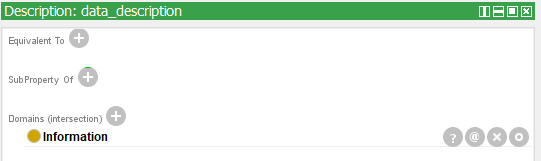
\includegraphics[width=10cm]{../../Images/04_Contribution/04_data_description.png}
  \caption{If $Information$ is the domain of the property $data\_description$, then the reasoner will infer individuals that have a $data\_description$ as $Information$.}
  \label{fig:04_data_description}
\end{figure}

\paragraph{Inconsistency}
Code sample \ref{GODP_COMP} presents the generic ontology design pattern to create a data property. This code sample includes a range. The definition of the range limits the data range that the data property accepts, for example, a $xsd:string$ accepts strings or $xsd:int$ accepts integers. The ontology is inconsistent when the data property stores a value that is outside of the defined range.

\paragraph{Generic ontology design pattern}
Code sample \ref{GODP_COMP} adds a data property or an object property to an existing class. We use three parameters to instantiate the data or object property: $c$ defines the class that should host the data property, $p$ defines the data property itself, and $r$ defines the range of the data property. We use the range of the data property to restrict its content using, for example, regular expressions and use the range of the object property to infer the class of an individual. Figure \ref{fig:GODP_COMP_DP} presents the data property, and figure \ref{fig:GODP_COM_OP} presents the object property.

\begin{lstlisting}[float,language=GDOL,caption={The GDOL code for adding a required data property to an existing class using two parameters. We use $c$, $i$, and $r$ as parameters to instantiate the data or object property.},label={GODP_COMP}][H]
pattern Completeness_dp [Class: c; DataProperty: i; Datatype: r] =
	DataProperty: i Domain: c Range: r
pattern Completeness_op [Class: c; ObjectProperty: i; Datatype: r] =
	ObjectProperty: i Domain: c Range: r
\end{lstlisting}

\begin{figure}[H]
\centering
  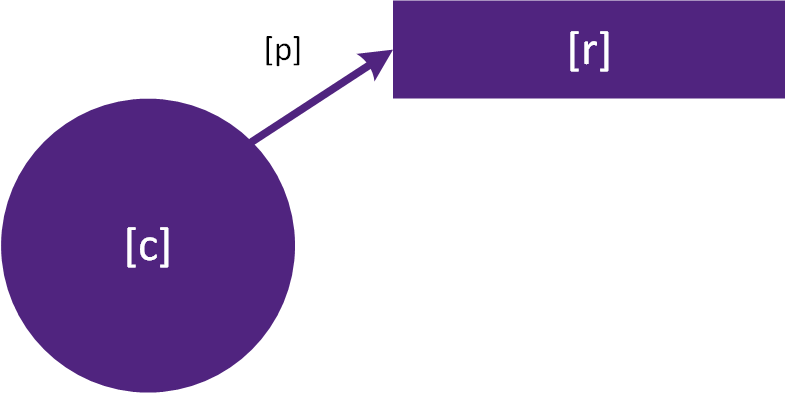
\includegraphics[width=5cm]{../../Images/04_Contribution/Completeness_DP.png}
  \caption{The completeness of a class using a data property. Code sample \ref{GODP_COMP} presents the GDOL code for adding a data property to an existing class. Code sample \ref{GODP_COMP} presents the GDOL code that instantiates this ontology.}
  \label{fig:GODP_COMP_DP}
\end{figure} 

\begin{figure}[H]
\centering
  
\includegraphics[width=6cm]{../../Images/04_Contribution/Completeness_OP.png}
  \caption{The completeness of a class using an object property. Code sample \ref{GODP_COMP} presents the GDOL code for adding an object property to an existing class. Code sample \ref{GODP_COMP} presents the GDOL code that instantiates this ontology.}
  \label{fig:GODP_COM_OP}
\end{figure} 

\paragraph{Constraints}
The SHACL shape in code sample \ref{SHACL_COM_DP} detects when an individual classified as $c$ does not host the defined data or object property $p$. Each individual classified as $c$ should have at least one path (object or data property) $p$. The SHACL shape monitors the existence of the data or object property using the cardinality constraint $minCount$. $c$ and $p$ set the context of the constraints.

\begin{lstlisting}[float,language=SHACL,caption={The SHACL code that validates if the individuals classified as $c$ host the property $p$. We use the cardinality constraint $sh:minCount$ for this detection: each individual classified as $c$ should have at least one path (object or data property) $p$.},label={SHACL_COM_DP}][H]
[c]Shape a sh:NodeShape;
	sh:targetClass [c]; 
	sh:property [
		sh:path [p]; 
		sh:severity sh:Violation; 
		sh:minCount 1; 
		sh:message "Completeness: add [c] to [p]."; ]
\end{lstlisting} 
\subsubsection{Reproducibility} \label{odp_reproducibility}
% Subsection structure:
% Problem: what is the generalized problem?
% 	Motivation: why is this problem scientifically important and/or interesting?
% Solution: conceptual description of solution, including formal definition of GODP and SHACL shapes.
% 	Illustration: images of GODP structure.
% 	(Statistical)Analysis: how does the solution solve the problem?
% 	Evaluation: are the results significant? What is the impact?
\paragraph{Detecting reproducibility}
We use reproducibility to evaluate the reliability of decision-relevant information. The reproducibility pattern can detect when information cannot be traced back to an evidence source. When evidence cannot be traced back to an evidence source, the pattern detects the information as premature. 

\begin{center}
\large\color{document}{The reproducibility pattern validates the information reliability by detecting when information cannot be traced back to an evidence source.}
\end{center}

\paragraph{Ontology}
Information is reproducible when it can be traced back to evidence or an information source, for example, a contextual circumstance or the value of a stakeholder. This pattern relates information to an evidence source using an object property. An information class can be based on another information class as well, as long as the chain of information is evidence-based. We use the completeness pattern to ensure the required data properties are available. Figure \ref{fig:reproducibility_chain} presents a chain that connects information to evidence. The $based\_on\_in{\f}ormation$ object property is transitive. When we base information $a$ on information $b$, and information $b$ on information $c$, then information $a$ is also based on information $c$. We need the transitive characteristic to query the evidence sources of information for the decision presentation pattern.

\begin{figure}[H]
\centering
  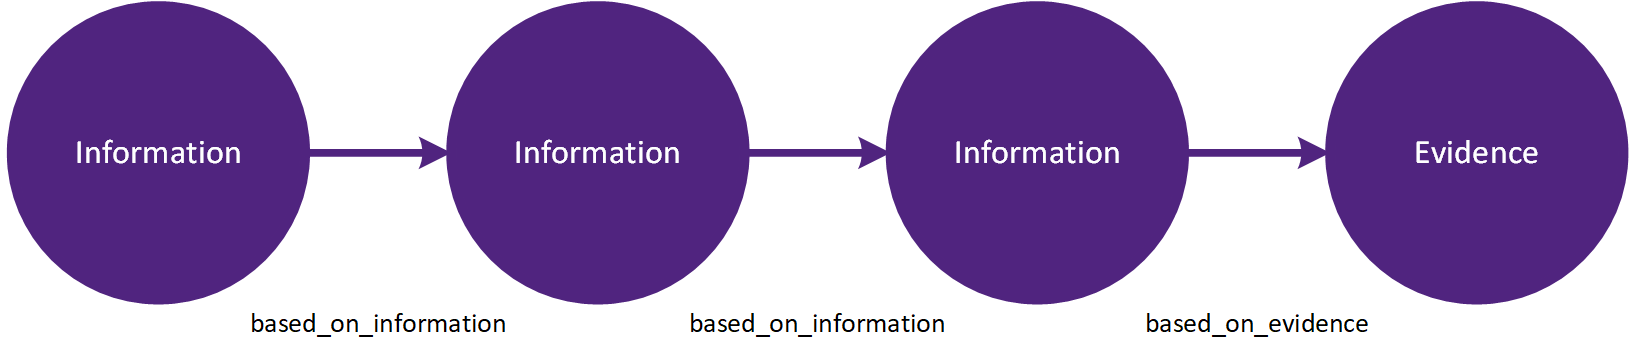
\includegraphics[width=13cm]{../../Images/Reproducibility_Chain.png}
  \caption{An example of an evidence-based chain of information. The reproducibility pattern should detect if the information in the chain is not evidence-based.}
  \label{fig:reproducibility_chain}
\end{figure} 

We extend the evidence-based management pattern in two ways:
\begin{enumerate}
\item Contextual circumstances and evaluated external evidence naturally refer to their actual evidence source, for example, a scientific article or an observation. Stakeholder evidence requires a specific stakeholder as a source of evidence. We extend the evidence-based management pattern with one class ($Stakeholder$) and the related object property ($shared\_by$). 
\item Individuals (classified as $In{\f}ormation$) hosting data properties should be evidence-based or information-based. The object property $based\_on\_evidence$ relates a class to the evidence class. The object property $based\_on\_in{\f}ormation$ relates a class to an information class. 
\end{enumerate} 

Figure \ref{fig:reproducibility} presents the resulting ontology. We have marked the extensions of the evidence-based management pattern in \textcolor{DarkBlue}{blue}.

\begin{figure}[H]
\centering
  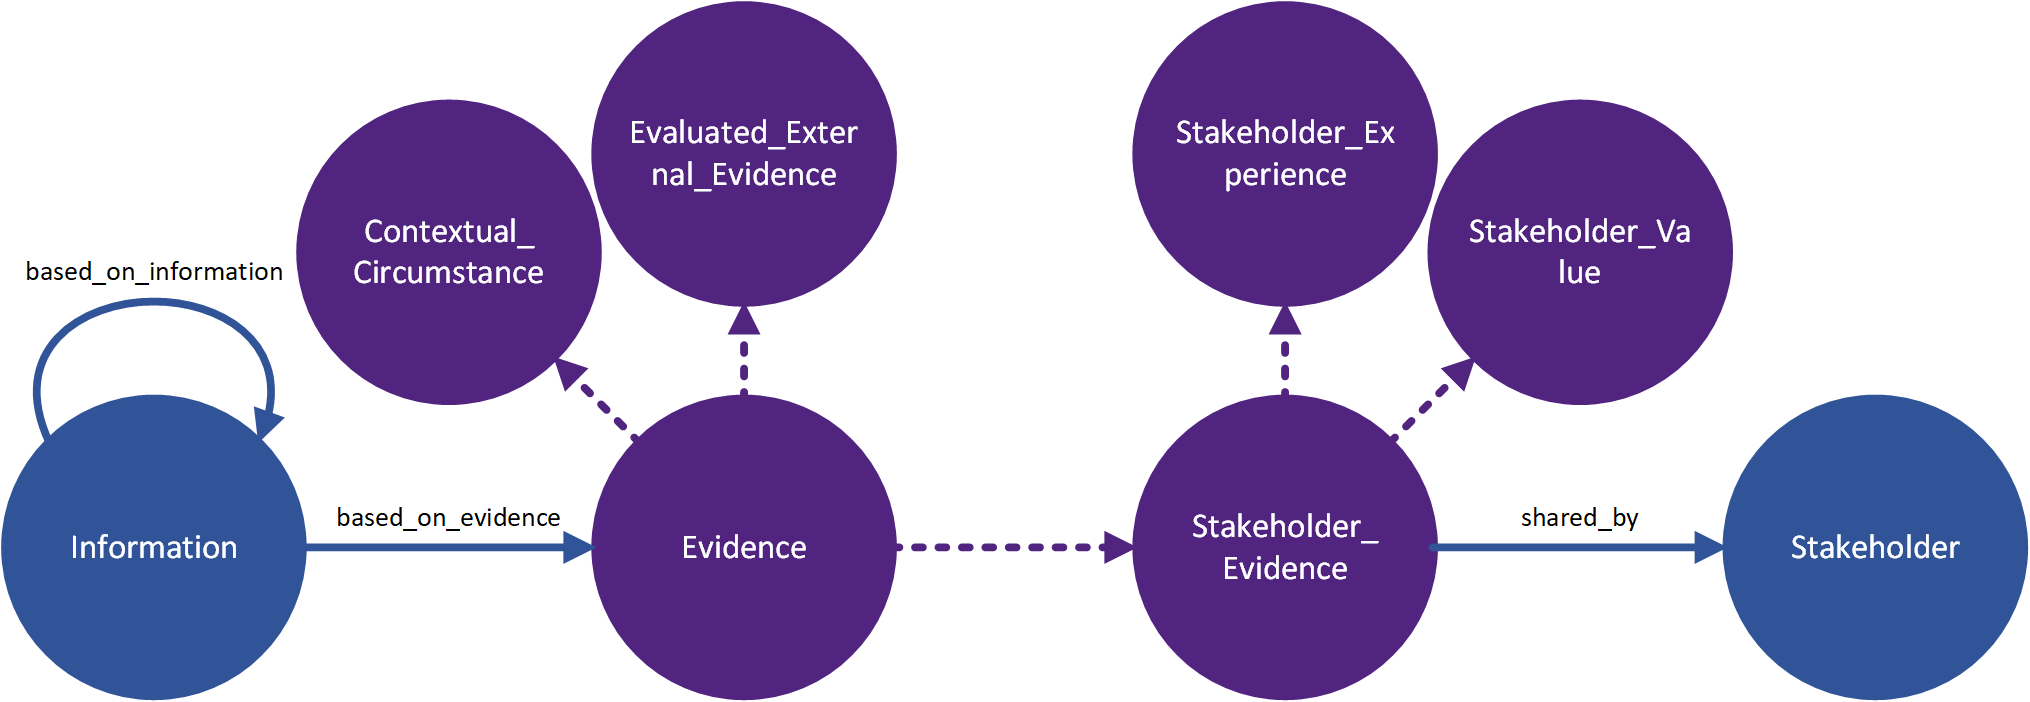
\includegraphics[width=14cm]{../../Images/04_Contribution/04_Reproducibility_Ontology.png}
  \caption{The reproducibility ontology. We have marked the extensions of the evidence-based management pattern in \textcolor{DarkBlue}{blue}. Code sample \ref{GODP_REP_EXT} presents the GDOL code that we use to instantiate this pattern.}
  \label{fig:reproducibility}
\end{figure}

\paragraph{Inferencing}
We use the domain and range of the $based\_on\_information$, $based\_on\_evidence$, and $shared\_by$ object properties to allow the reasoner to classify individuals that are using these object properties. Table \ref{table:rep_inference} presents the classification the reasoner infers from the domain and range configuration.

\begin{table}[H]
\centering
\caption{We use the domain and range of the $based\_on\_in{\f}ormation$, $based\_on\_evidence$, and $shared\_by$ object properties to allow the reasoner to classify individuals that are using these object properties.}
\begin{tabular}{| p{4cm} | p{6cm} |  p{4cm} |   }
\hline
\rowcolor{document}
\color{documentText}Domain & \color{documentText}Object property & \color{documentText}Range \\
\hline
$In{\f}ormation$ & $based\_on\_in{\f}ormation$ & $In{\f}ormation$ \\
\hdashline
$In{\f}ormation$ & $based\_on\_evidence$ & $Evidence$ \\
\hdashline
$Stakeholder\_Evidence$ & $shared\_by$ & $Stakeholder$ \\
\hline
\end{tabular}
\label{table:rep_inference}
\end{table}

\paragraph{Inconsistency} \label{rep_incons}
We guard the consistency of the ontology using $DisjointClasses$. The reasoner cannot classify an individual as $Information$ and $Evidence$ at the same time. If we allow the reasoner to do this, it might create a circular dependency in the reproducibility chain figure \ref{fig:reproducibility_chain} presents. $In{\f}ormation$ typically represents a statement that we can trace back to at least one $Evidence$ source. Code sample \ref{GODP_REP_EXT} presents the implementation of the $DisjointClasses$.

\paragraph{Generic ontology design pattern}
Figure \ref{fig:reproducibility} presents an ontology that extends the evidence-based management ontology and enables the detection of unreproducible information. Code sample \ref{GODP_REP_EXT} presents the GDOL code that extends the evidence-based management ontology. 

\begin{lstlisting}[float,language=GDOL,caption={The GDOL code for relating information to evidence and stakeholder evidence to a stakeholder. We introduce two new classes ($Stakeholder$ and $Information$) and three new object properties ($shared\_by$, $based\_on\_evidence$, and $based\_on\_in{\f}ormation$. Additionally, we define that $Information$ and $Evidence$ are disjoint. Figure \ref{fig:reproducibility} visualises the result of executing the code.},label={GODP_REP_EXT}][H]
ontology Reproducibility_Basic = EBM then 
 Class: Stakeholder 
 Class: Information 
 ObjectProperty shared_by Domain: Stakeholder_Evidence Range: Stakeholder 
 ObjectProperty based_on_evidence Domain: Information Range: Evidence
 ObjectProperty based_on_information Domain: Information Range: Information Characteristics: Transitive
 DisjointClasses: Information, Evidence
\end{lstlisting}

The classes that store decision-relevant information are required to be a subclass of $In{\f}ormation$. Code sample \ref{GODP_REP_EV} presents the GDOL code that relates information to evidence. The inferencing using the domain and range of the $based\_on\_in{\f}ormation$, $based\_on\_evidence$, and $shared\_by$ object properties contributes to this classification as well.

\begin{lstlisting}[float,language=GDOL,caption={The GDOL code that classifies individuals as a sub-class of $Information$. We use $dri$ (decision relevant information) and $i$ (information) as parameters.},label={GODP_REP_EV}][H]
pattern Reproducibility_Context [Class: dri; Class: i] = 
 Class: [dri] SubClassOf: [i]
\end{lstlisting}

\paragraph{Constraints}
Code sample \ref{SHACL_REP} presents the SHACL shape that detects unreproducible information. Each individual that is classified as $In{\f}ormation$ is required to host the object property $based\_on\_in{\f}ormation$ or $based\_on\_evidence$. Individuals that are classified as $In{\f}ormation$ can be traced back to an evidence or information source by hosting one of these two object properties. If the individual does not host one of the object properties, its information cannot be traced back to an evidence source, and the pattern detects the information as premature. The SHACL shape monitors the existence of the object properties using the cardinality constraint $minCount$. 

\begin{lstlisting}[float,language=SHACL,caption={The SHACL code that detects if $Information$ is not $based\_on\_evidence$ or $based\_on\_in{\f}ormation$. The SHACL shape monitors the existence of these object properties using the cardinality constraint $minCount$. },label={SHACL_REP}][H]
Used_InformationShape a sh:NodeShape;
	sh:targetClass Information; 
	sh:property [
		sh:or (
			[sh:path based_on_information; sh:minCount 1;]
			[sh:path based_on_evidence; sh:minCount 1;]
		)
		sh:severity sh:Violation; 
		sh:message "Reproducibility: enter an information or evidence source for this information."; ];
\end{lstlisting}

Code sample \ref{SHACL_REP_SH} presents the SHACL shape that detects when the pattern cannot trace back $Stakeholder\_Experience$ or a $Stakeholder\_Value$ to a $Stakeholder$. We use the $shared\_by$ combined with the cardinality constraints $sh:minCount$ object property to achieve this. The constraints generate a violation if an individual that is classified as $Stakeholder\_Evidence$ is not $shared\_by$ a stakeholder.

\begin{lstlisting}[float,language=SHACL,caption={The SHACL code that detects when a stakeholder does not share $Stakeholder\_Evidence$. We use the cardinality constraint $sh:minCount$ for this detection: each individual classified as $Stakeholder\_Evidence$ should have at least one path $shared\_by$. The range of $shared\_by$ is $Stakeholder$.},label={SHACL_REP_SH}][H]
StakeholderShape a sh:NodeShape;
	sh:targetClass Stakeholder_Evidence; 
	sh:property [
		sh:path shared_by;
		sh:severity sh:Violation; 
		sh:minCount 1; 
		sh:message "Reproducibility: enter a stakeholder that serves as the source of this stakeholder evidence."; ];
\end{lstlisting} 
\subsubsection{Consensus} \label{odp_consensus}
% Subsection structure:
% Problem: what is the generalized problem?
% 	Motivation: why is this problem scientifically important and/or interesting?
% Solution: conceptual description of solution, including formal definition of GODP and SHACL shapes.
% 	Illustration: images of GODP structure.
% 	(Statistical)Analysis: how does the solution solve the problem?
% 	Evaluation: are the results significant? What is the impact?
\paragraph{Detecting consensus}
Information that is based on multiple evidence sources is more reliable than information that is based on one evidence source. For example, one scientific paper supported by stakeholder experience is more reliable than a scientific paper alone. 

\begin{center}
\large\color{document}{The consensus pattern validates the evidence reliability by detecting when evidence does not agree with at least one additional evidence source.}
\end{center}

\paragraph{Ontology}
We define consent evidence as evidence that agrees with at least one other evidence source. The reproducibility pattern provides the structure on which we create the consensus pattern. We introduce the $agrees\_with$ object property. Figure \ref{fig:consensus} presents the consensus pattern. We mark the extension of the reproducibility pattern in \textcolor{LightGreen}{green}. For example, if two stakeholders have the same experience, the $agrees\_with$ object property can link this stakeholder experience. 

\begin{figure}[H]
\centering
  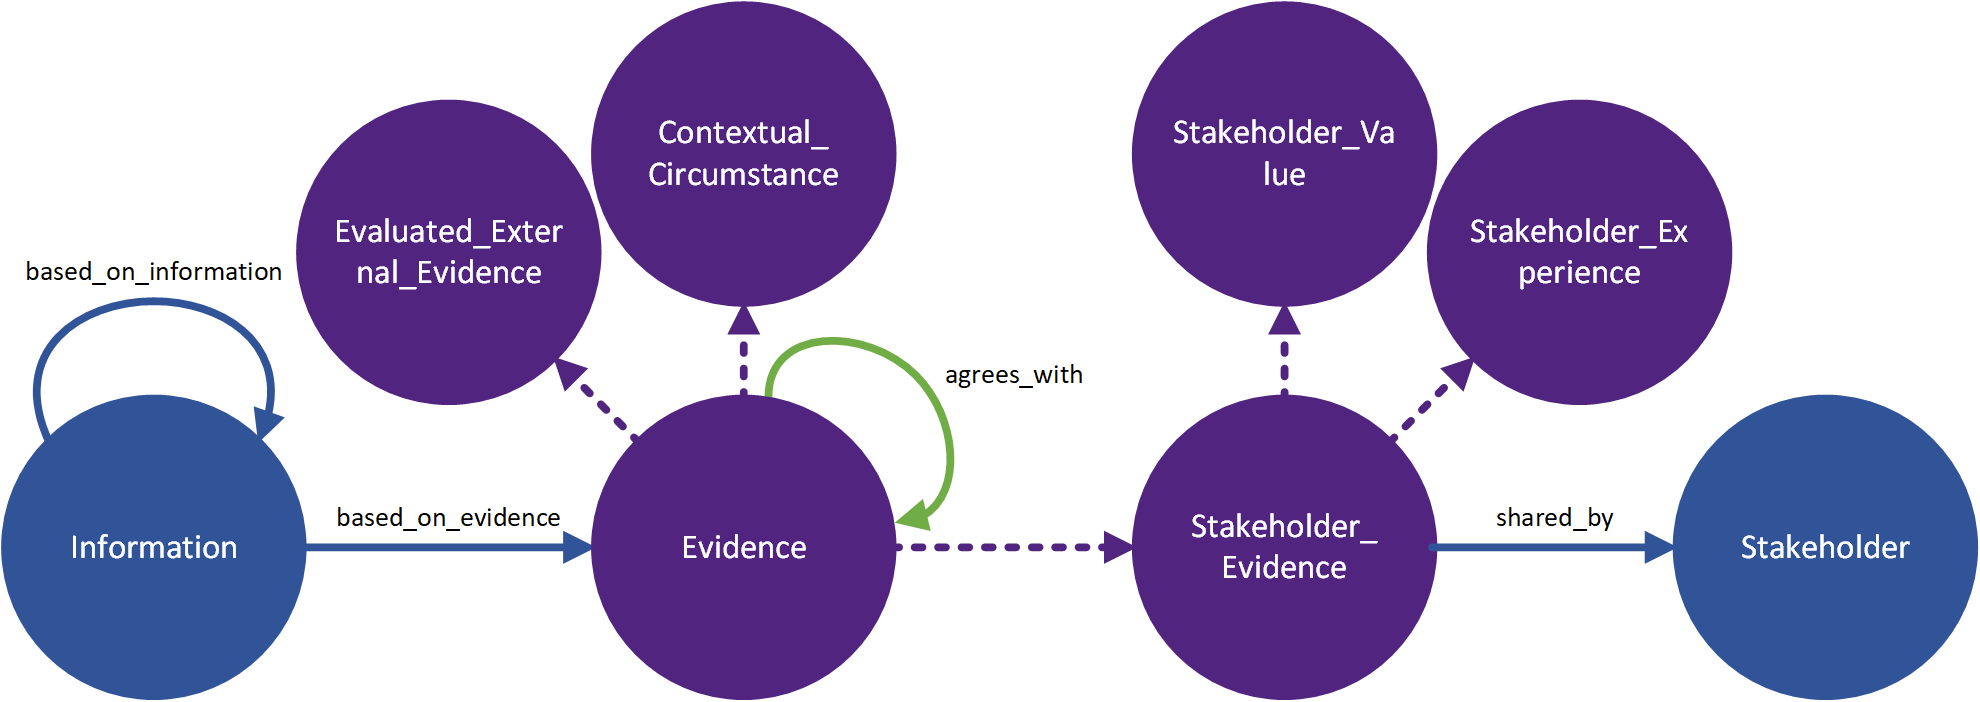
\includegraphics[width=14cm]{../../Images/04_Contribution/04_Consensus_Ontology.png}
  \caption{The consensus pattern that we have based on the reproducibility pattern. We have extended the reproducibility pattern with the object property $agrees\_with$. Code sample \ref{GODP_CON_LEV} extends the reproducibility pattern using GDOL.}
  \label{fig:consensus}
\end{figure}

\paragraph{Inferencing}
We can measure the consensus-level of an evidence source using the $agrees\_with$ object property. We extend the $based\_on\_evidence$ object property with a super property. When we base $In{\f}ormationX$ on $EvidenceA$, and $EvidenceA$ agrees with $EvidenceB$, the reasoner bases $In{\f}ormationX$ on $EvidenceB$ as well. Figure \ref{fig:consensus_inferred} presents the super property that infers this knowledge from the existing ontology structure.

\begin{figure}[H]
\centering
  
\includegraphics[width=17cm]{../../Images/Consensus_Inferred.png}
  \caption{The super property that infers the object property $based\_on\_evidence$ in Prot\'eg\'e.}
  \label{fig:consensus_inferred}
\end{figure}

The $agrees\_with$ object property is symmetric. If individual $A$ agrees with individual $B$, individual $B$ should also agree with individual $A$. Figure \ref{fig:consensus_transitive} presents the characteristics of the $agrees\_with$ object property.

\begin{figure}[H]
\centering
  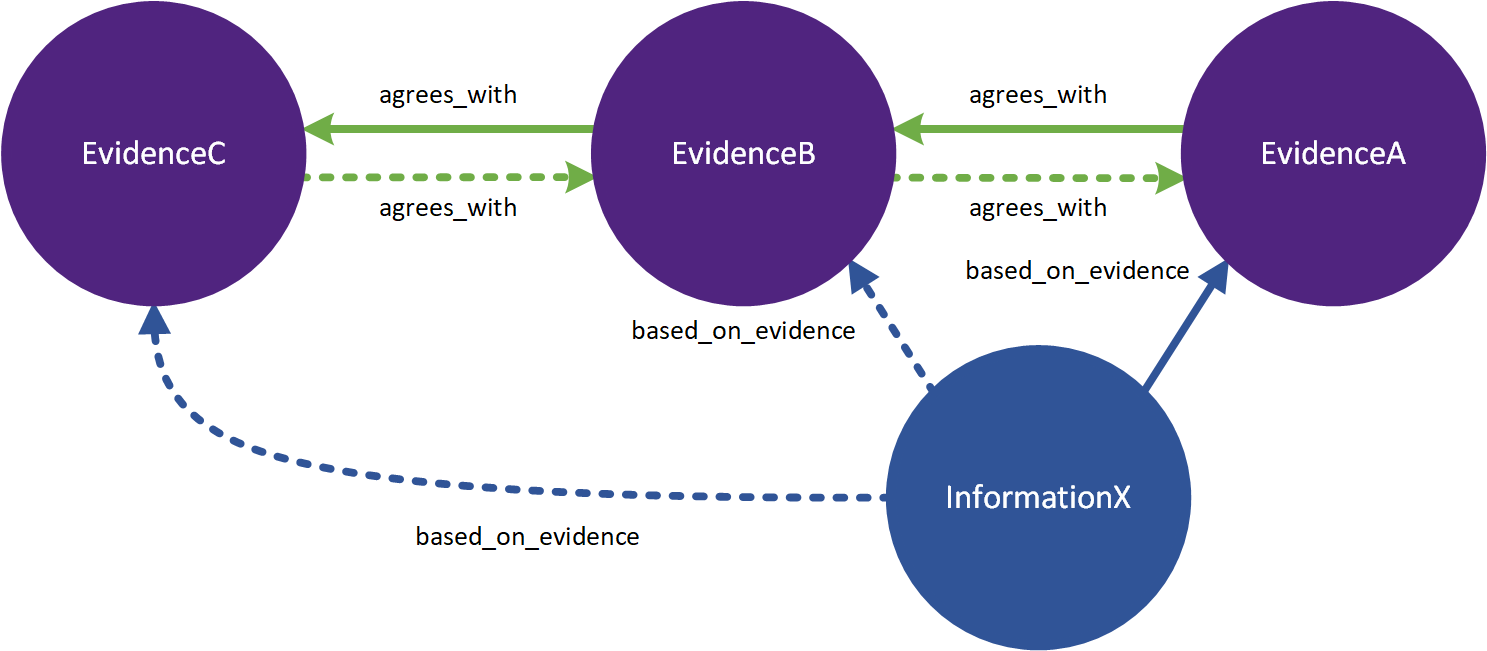
\includegraphics[width=13cm]{../../Images/04_Contribution/04_Consensus_Characteristics.png}
  \caption{An example of the impact of the symmetric characteristics of the $agrees\_with$ object property. The reasoner infers the dotted lines based on the super property figure \ref{fig:consensus_inferred} presents and the symmetric characteristics of $agrees\_with$.}
  \label{fig:consensus_transitive}
\end{figure}

\paragraph{Inconsistency}
The consensus pattern inherits the consistency validation from the reproducibility pattern. We describe the consistency of the reproducibility pattern in section \ref{rep_incons} \nameref{rep_incons}.

\paragraph{Generic ontology design pattern}
Code sample \ref{GODP_CON_LEV} presents the described solution into GDOL. We take the $Reproducibility\_Basic$ pattern, introduce the $agrees\_with$ object property, and extend the $based\_on\_evidence$ object property. 

\begin{lstlisting}[float,language=GDOL,caption={The GDOL code that extends the reproducibility pattern and results in the consensus pattern. We take the $Reproducibility\_Basic$ pattern, introduce the $agrees\_with$ object property, and extend the $based\_on\_evidence$ object property. Figure \ref{fig:consensus} presents the generic ontology design pattern.},label={GODP_CON_LEV}][H]
ontology Consensus = Reproducibility_Basic then
 ObjectProperty: agrees_with Domain: Evidence Range: Evidence Characteristics: Symmetric
 ObjectProperty: based_on_evidence SubPropertyChain: based_on_evidence o agrees_with SubPropertyOf: based_on_evidence
\end{lstlisting}

\paragraph{Constraints}
We define one consensus level for each individual classified as $Evidence$. We set the consensus-level to $1$. This consensus level ensures that each used evidence source has at least one other agreeable evidence source. The minimum consensus level can be adjusted depending on the environment. For example, in life-safety environments, the consensus level might be increased. We use the cardinality constraint $sh:minCount$ for the consensus detection: each individual classified as $Evidence$ should have at least one path $agrees\_with$.

\begin{lstlisting}[float,language=SHACL,caption={The SHACL shapes that detect when information does not meet the minimum consensus level.},label={SHACL_CON_LEV}][H]
UsedEvidenceShape a sh:NodeShape;
	sh:targetClass Evidence; 
	sh:property [
		sh:path agrees_with; 
		sh:severity sh:Violation; 
		sh:minCount 1; 
		sh:message "Consensus: ensure the evidence is in agreement with at least one additional evidence source."; ];
\end{lstlisting} 
\subsubsection{Conflict} \label{odp_conflict}
% Subsection structure:
% Problem: what is the generalized problem?
% 	Motivation: why is this problem scientifically important and/or interesting?
% Solution: conceptual description of solution, including formal definition of GODP and SHACL shapes.
% 	Illustration: images of GODP structure.
% 	(Statistical)Analysis: how does the solution solve the problem?
% 	Evaluation: are the results significant? What is the impact?
\paragraph{Detecting conflict}
Information that has conflicting evidence sources is less reliable compared to information that does not have conflicting evidence sources. For example, stakeholder experience that is conflicting with evaluated external evidence is less reliable compared to stakeholder experience that does not have any conflict. We define the number of evidence sources that causes a conflict with the decision-relevant information as the level of conflict. We define the level of conflict using the reproducibility of information. When information is reproducible by one evidence source, and this evidence source has one additional conflicting evidence source, the level of conflict is $1$. When the evidence source has two conflicting evidence sources, the level of conflict is $2$. Compared to a fuzzy approach that can classify certain conflict levels as, for example, $low$, $medium$, or $high$, the number-based approach makes it easier to compare conflict levels. We do not compare conflict-levels in this study.

\begin{center}
\large\color{document}{The conflict pattern validates information reliability by detecting conflicting evidence.} 
\end{center}

\paragraph{Ontology}
We define conflicting evidence as evidence that disagrees with another evidence source. The reproducibility pattern serves as a natural base for the conflict pattern. The reproducibility pattern provides the structure on which we create the conflict pattern using the object property $disagrees\_with$. Figure \ref{fig:conflict} presents the conflict pattern. We mark the extension of the conflict pattern in \textcolor{Red}{red}. We measure the level of conflict between evidence sources using the $disagrees\_with$ object property. For example, if two stakeholders have a different experience, the $disagrees\_with$ object property represents this conflicting stakeholder experience. 

\begin{figure}[H]
\centering
  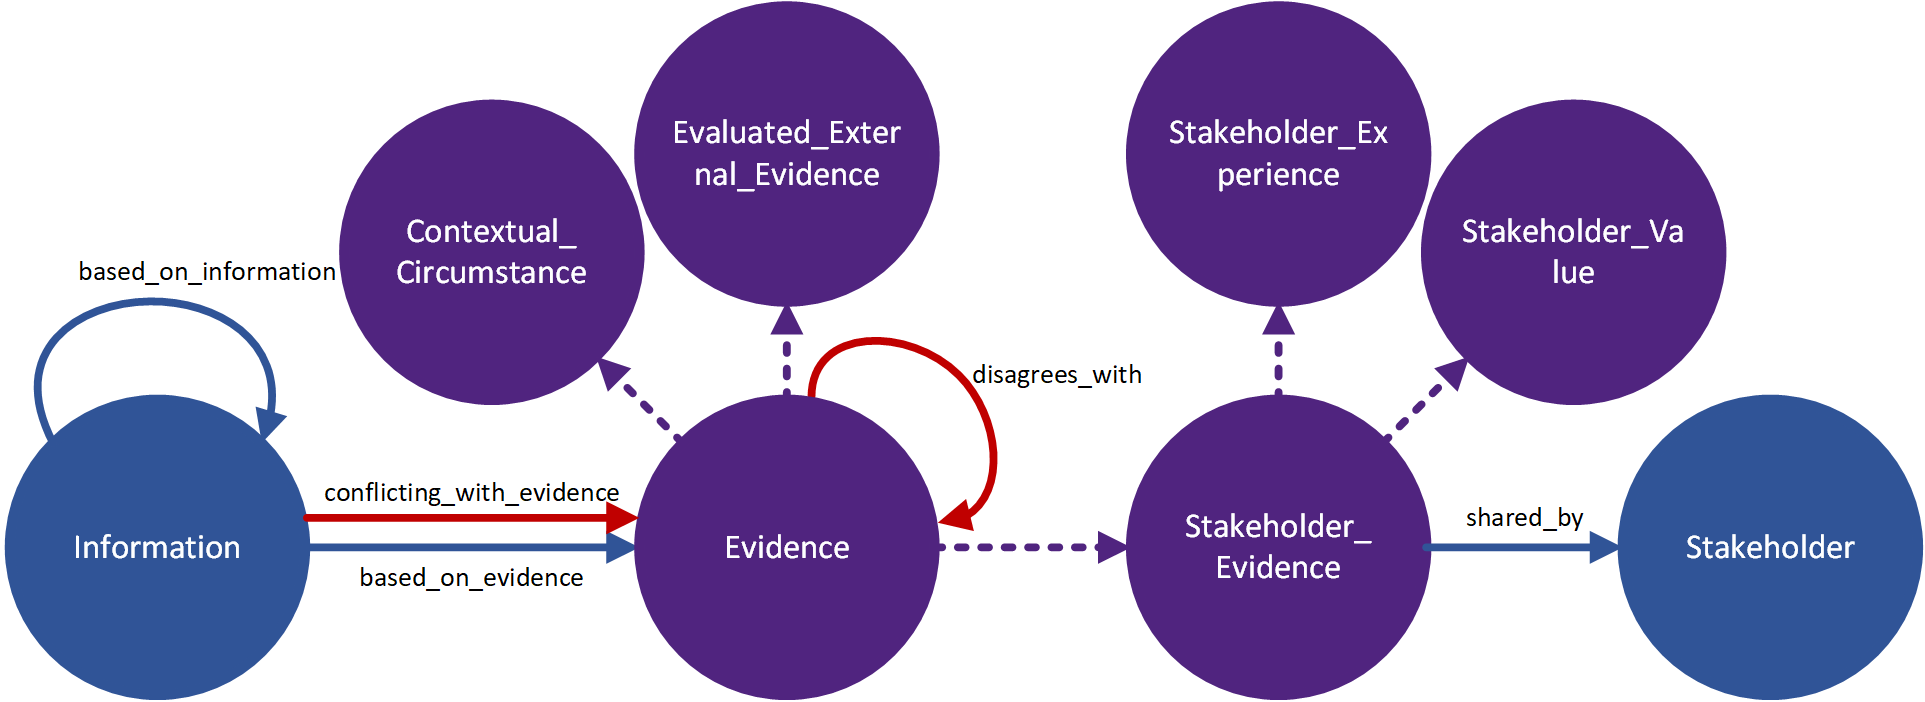
\includegraphics[width=14cm]{../../Images/04_Contribution/04_Conflict_Ontology.png}
  \caption{The conflict pattern uses the reproducibility pattern and extends it with the object property $disagrees\_with$. Code sample \ref{GODP_CONF_LEV} presents the GDOL code for instantiating the conflict pattern.}
  \label{fig:conflict}
\end{figure}

\paragraph{Inferencing}
We introduce an additional object property: $conflict\_with\_evidence$. When we base $In{\f}ormationX$ on $EvidenceA$, and $EvidenceA$ disagrees with $EvidenceB$, $In{\f}ormationX$ conflicts with $EvidenceB$. This conflict reduces trust in $In{\f}ormationX$. Figure \ref{fig:conflict_inferred} presents the super property that infers this knowledge from the existing ontology structure.

\begin{figure}[H]
\centering
  
\includegraphics[width=17cm]{../../Images/Conflict_Inferred.png}
  \caption{The configuration of the super property that infers the object property $conflict\_with\_evidence$ in Prot\'eg\'e.}
  \label{fig:conflict_inferred}
\end{figure}

$disagrees\_with$ is symmetric and irreflexive. Disagreement is always symmetric: if $StakeholderA$ disagrees with $StakeholderB$ on a specific subject, then $StakeholderB$ also disagrees with $StakeholderA$. Figure \ref{fig:conflict_irreflexive} presents the situation in which $disagrees\_with$ is symmetric and irreflexive.

\begin{figure}[H]
\centering
  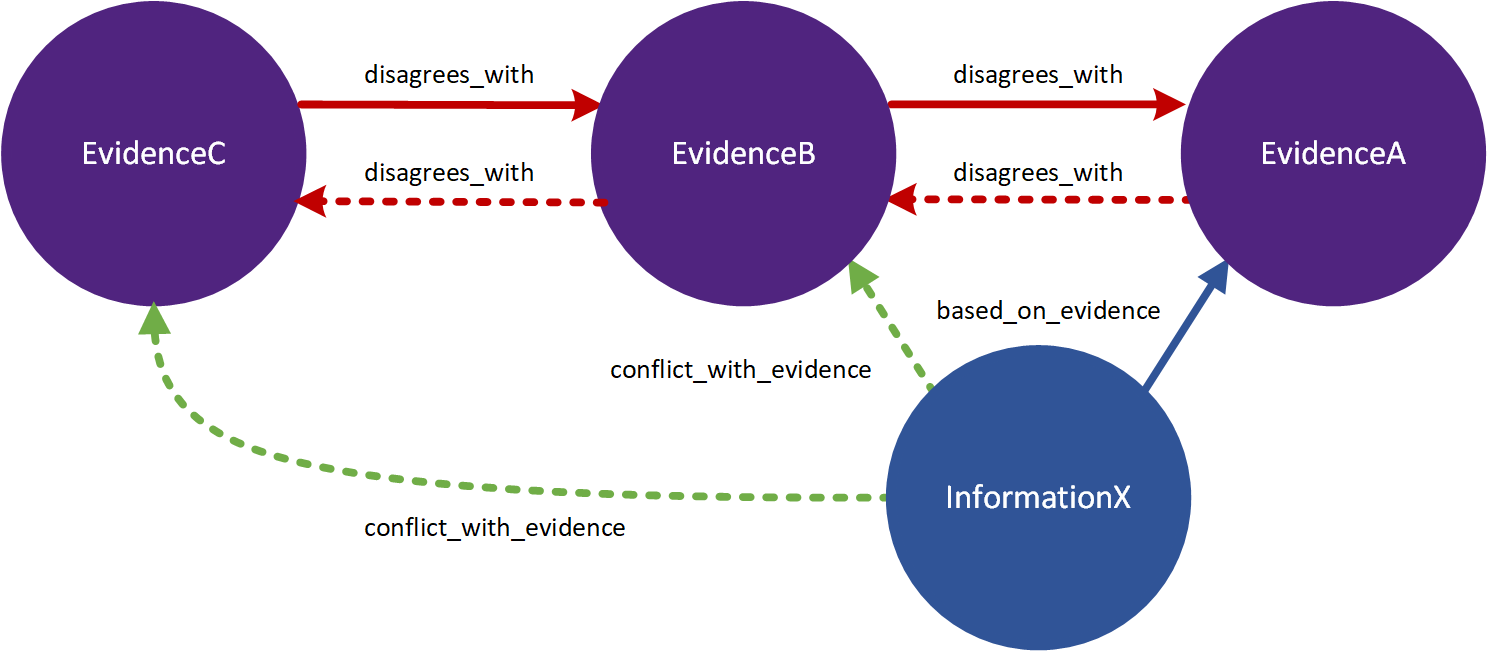
\includegraphics[width=13cm]{../../Images/04_Contribution/04_Conflict_Characteristics.png}
  \caption{The symmetric and irreflexive characteristics of $disagrees\_with$. The reasoner infers the dotted lines based on the super property figure \ref{fig:conflict_inferred} presents.}
  \label{fig:conflict_irreflexive}
\end{figure}

\paragraph{Inconsistency}
The consensus pattern inherits the consistency validation from the reproducibility pattern. We describe the consistency of the reproducibility pattern in section \ref{rep_incons} \nameref{rep_incons}.

Figure \ref{fig:conflict_transitive} presents the hypothetical situation in which $disagrees\_with$ is symmetric, transitive, and irreflexive. This situation results in an inconsistent ontology. The reasoner infers the $disagrees\_with$ object property on $EvidenceA$ based on the transitivity characteristic. This object property causes conflict with the irreflexive character of $disagrees\_with$. The transitivity helps us to discover disagreement chains and ensures we present the right conflict level to the decision-maker. Transitivity causes a problem: evidence cannot disagree with itself. When we combine the irreflexive and transitive characteristics, the reasoner might infer the $disagrees\_with$ object property on an evidence source. For example, we assume $R$ is transitive and irreflexive. By transitivity, we conclude $xRy \land yRx \rightarrow xRx$. However, this is not possible as $R$ should be irreflexive as well.

\begin{figure}[H]
\centering
  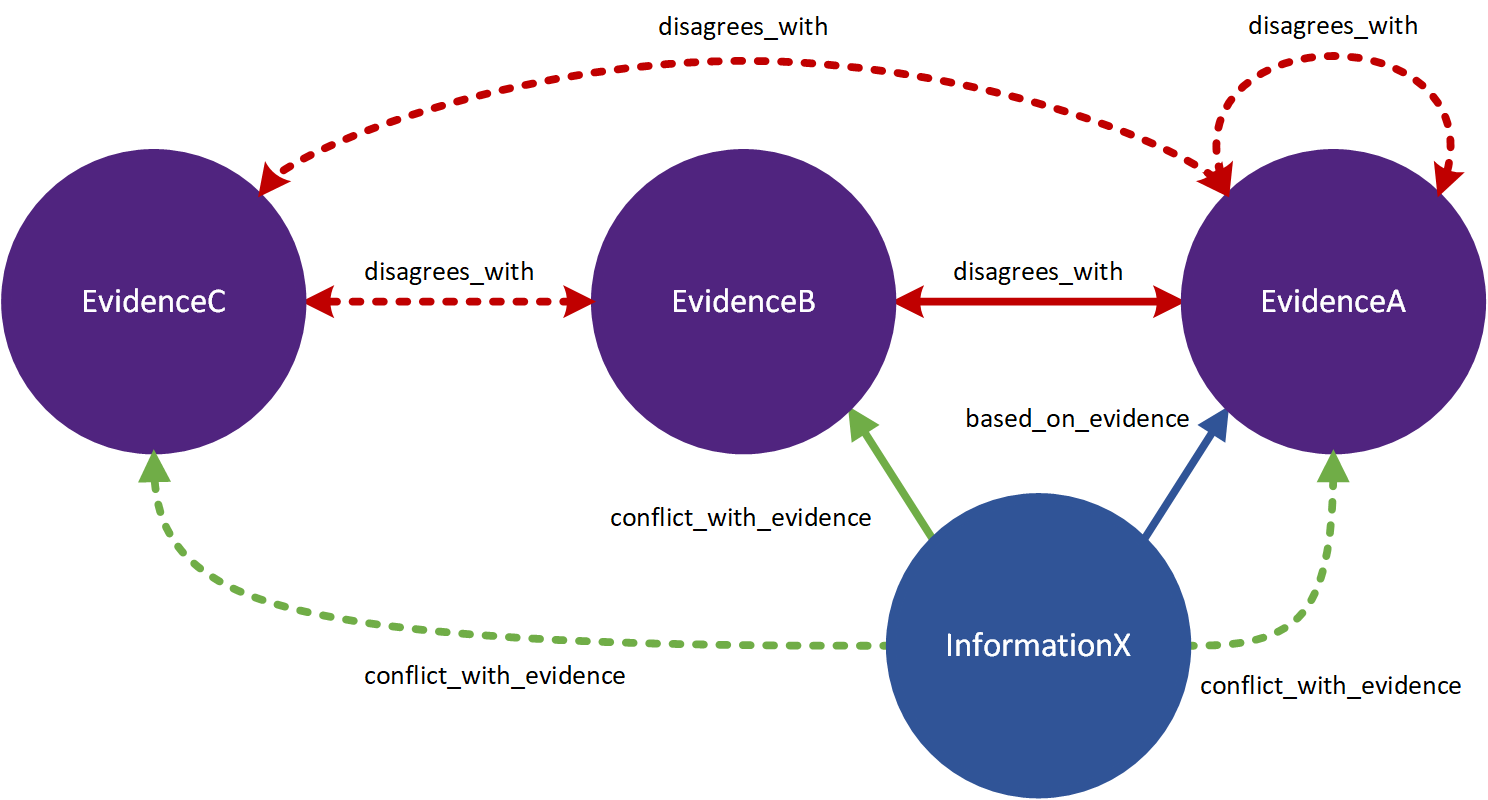
\includegraphics[width=13cm]{../../Images/Conflict_Transitive.png}
  \caption{The transitive characteristic of $disagrees\_with$ causes an inconsistent ontology. The reasoner infers the dotted lines based on the super property figure \ref{fig:conflict_inferred} presents.}
  \label{fig:conflict_transitive}
\end{figure}

\paragraph{Generic ontology design pattern}
Code sample \ref{GODP_CONF_LEV} presents the described solution into GDOL. We take the $Reproducibility\_Basic$ pattern and add the $disagrees\_with$ and $conflict\_with\_evidence$ object properties.

\begin{lstlisting}[float,language=GDOL,caption={The GDOL code that extends the reproducibility pattern and results in the conflict pattern. We take the $Reproducibility\_Basic$ pattern and add the $disagrees\_with$ and $conflict\_with\_evidence$ object properties.},label={GODP_CONF_LEV}][H]
ontology Conflict = Reproducibility_Basic then
  ObjectProperty: disagrees_with Domain: Evidence Range: Evidence Characteristics: Symmetric, Irreflexive
  ObjectProperty: conflict_with_evidence SubPropertyChain: based_on_evidence o disagrees_with SubPropertyOf: conflict_with_evidence
end
\end{lstlisting}

\paragraph{Constraints}
The conflict pattern requires the definition of a conflict level. Conflict reduces the reliability of the information and evidence. Therefore, we do not accept any conflict for our evidence and define the maximum conflict-level as $0$. Any conflict that the constraints detect immediately causes a violation. We use the cardinality constraint $sh:minCount$ for this detection: each individual classified as $In{\f}ormation$ should not have any path (object property) $conflict\_with\_evidence$.

\begin{lstlisting}[float,language=SHACL,caption={The SHACL shapes that detect if there is conflict. },label={SHACL_CONF_LEV}][H]
Used_InformationShape a sh:NodeShape;
	sh:targetClass Used_Information; 
	sh:property [
		sh:path conflict_with_evidence; 
		sh:severity sh:Violation; 
		sh:maxCount 0; 
		sh:message "Conflict detected. Please resolve the conflict or re-consider using this information."; ];
\end{lstlisting} 

\subsubsection{Pattern consolidation}
The decision ontology pattern reduces the complexity of the instantiation of the completeness, reproducibility, consensus, and conflict patterns.

\paragraph{Pattern dependencies}
We cannot reproduce information that does not exist. We validate the reproducibility of existing, and therefore, complete information. The consensus and conflict patterns have a similar dependency on the reproducibility pattern. When information is evidence-based, we can validate if the evidence agrees with other evidence (and define the level of consensus) or if information disagrees with other evidence (and define the level of conflict). 

\begin{center}
\large\color{document}{There is no consensus or conflict without reproducibility. There is no reproducibility without completeness.} 
\end{center}

\paragraph{Completeness and reproducibility using N-ary relations}
The completeness pattern validates the completeness of data properties and object properties. The reproducibility pattern validates the reproducibility of individuals using the object properties $based\_on\_evidence$ and $based\_on\_in{\f}ormation$. We need to relate a data property, containing decision-relevant information, to an object property. Figure \ref{fig:DecisionDesignPattern_NARY1} presents an example: $dataproperty1$ would be reproducible based on $based\_on\_evidence$. However, $dataproperty2$ would not be reproducible.

\begin{figure}[H]
\centering
  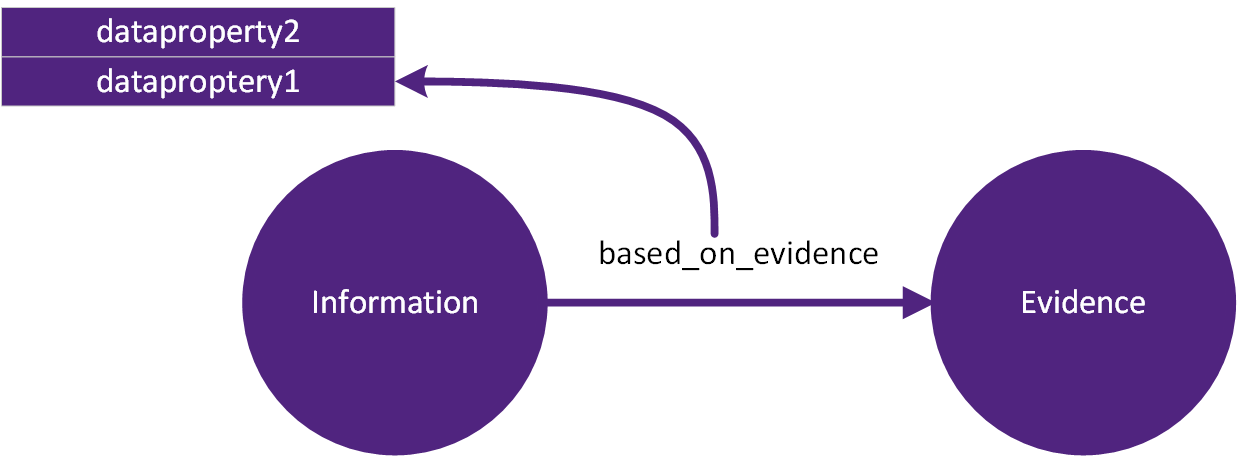
\includegraphics[width=10cm]{../../Images/04_Contribution/04_DecisionDesignPattern_NARY1.png}
  \caption{How can we reproduce $dataproperty1$ based on the object property $based\_on\_evidence$? However, $dataproperty2$ is not reproducible.}
  \label{fig:DecisionDesignPattern_NARY1}
\end{figure}

A property is a binary relation that relates two individuals \parencite{WEB16}. This concept makes it challenging to describe a relationship. In our case, we would describe the $based\_on\_evidence$ relationship with the data properties this relationship represents. We can describe object properties using annotations. Figure \ref{fig:DecisionDesignPattern_NARY2} presents the implementation of the annotation on the object property $based\_on\_evidence$ in Prot\'eg\'e, indicating that it $reproduces$ the $requirement\_cost$. 

\begin{figure}[H]
\centering
  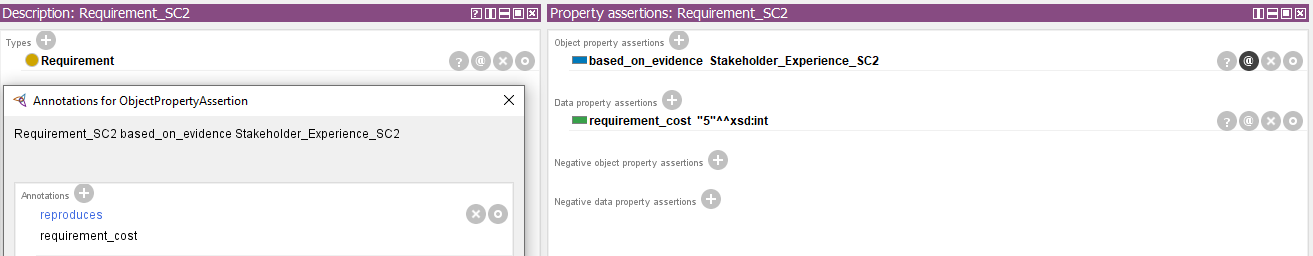
\includegraphics[width=16cm]{../../Images/04_Contribution/04_DecisionDesignPattern_NARY2.png}
  \caption{The implementation of the annotation on the object property $based\_on\_evidence$ in Prot\'eg\'e, indicating that it $reproduces$ the $requirement\_cost$.}
  \label{fig:DecisionDesignPattern_NARY2}
\end{figure}

However, annotation properties are merely descriptive and cannot define a characteristic of an object or data property \parencite{WEB12}. Therefore, the annotation properties are not suitable for inferencing or constraint validation. Additionally, we cannot use annotation properties to validate the reproducibility.

We define n-ary relations to solve this challenge \parencite{WEB16}. An n-ary relation introduces a new class for information that we would typically store in a data property. The new class hosts the actual information as data properties. We define three types of individuals for our purpose: $root$, $in{\f}ormation$, and $target$. The $root$ provides the context for the $in{\f}ormation$. The $in{\f}ormation$ stores the actual information in two data properties ($data\_value$ and $data\_description$), and the $target$ serves as the target for reproduction. We use the $data\_value$ to give an integer to the information. The $data\_description$ describes the value. We suggest setting the $data\_value$ to $0$ when the context does not require the use of the $data\_value$. Figure \ref{fig:root_information_target} presents the definitions.

\begin{figure}[H]
\centering
  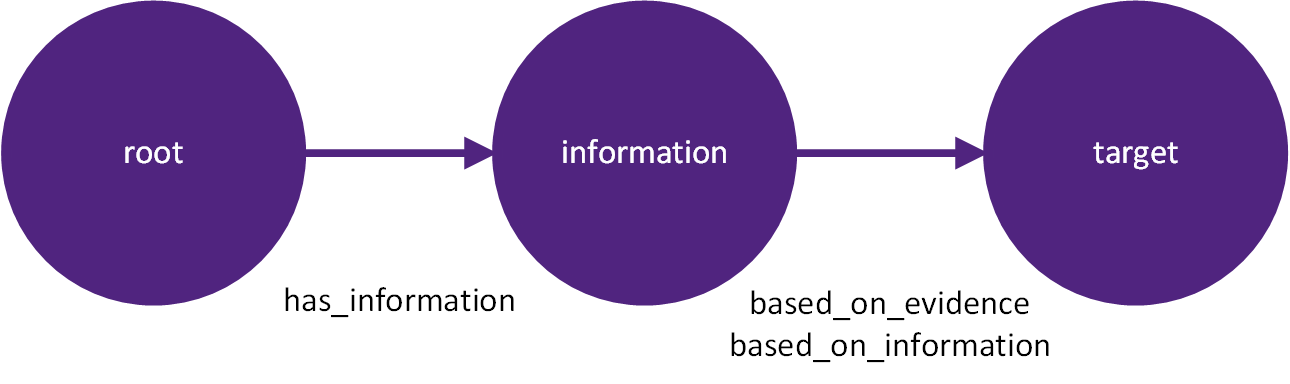
\includegraphics[width=10cm]{../../Images/04_Contribution/04_root_information_target.png}
  \caption{The $root$, $in{\f}ormation$, and $target$ individuals in n-ary relation.}
  \label{fig:root_information_target}
\end{figure}

Figure \ref{fig:DecisionDesignPattern_NARY3} presents an example of this concept. Class $r$, the root class, has two decision-relevant information properties: $n1$ and $n2$. These decision-relevant information properties have at least the $data\_value$ and $data\_description$ data properties. We classify them as $In{\f}ormation$. $n1$ and $n2$ are reproducible using the object properties $based\_on\_evidence$ or $based\_on\_in{\f}ormation$. We need to ensure that the completeness and reproducibility patterns function in this environment.

\begin{figure}[H]
\centering
  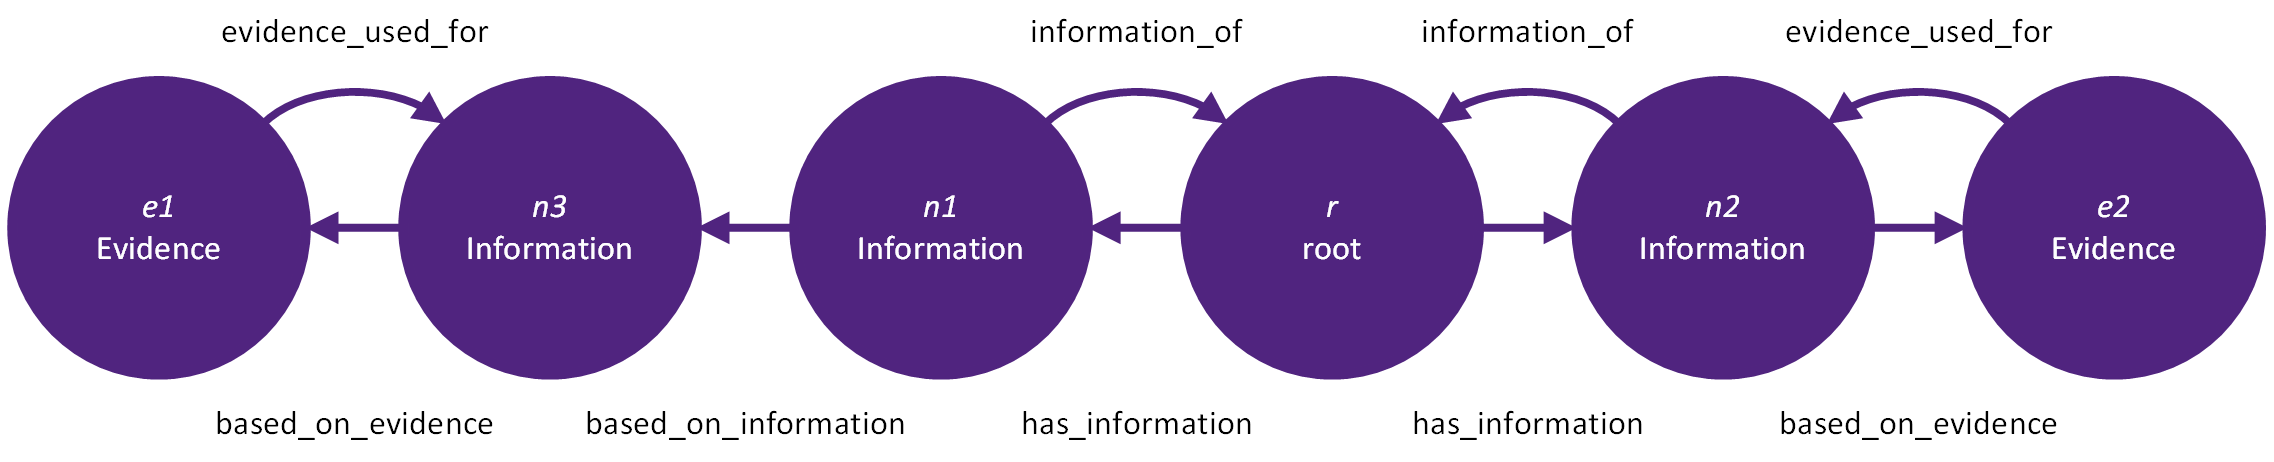
\includegraphics[width=17cm]{../../Images/04_Contribution/04_DecisionDesignPattern_NARY3.png}
  \caption{Class $r$ with two decision-relevant information properties: $n1$ and $n2$. These decision-relevant information properties have a $data\_value$ and a $data\_description$. $n1$ and $n2$ are reproducible using the object property $based\_on\_evidence$.}
  \label{fig:DecisionDesignPattern_NARY3}
\end{figure}

We validate the completeness of information using the $has\_information$ object property, including its range. We validate the reproducibility of information using the $based\_on\_evidence$ and $based\_on\_in{\f}ormation$ object properties.

\paragraph{\emph{Used} classes}
We use $Used\_*$ classes throughout the patterns to define the scope of the constraints. Each $Used\_*$ class is a subclass of its parent. We define the $Used\_*$ class in a way the reasoner classifies individuals that are relevant for the constraints. Figure \ref{fig:04_Used_Information} presents, for example, the $Used\_In{\f}ormation$ class. There might be a lot of individuals classified as $In{\f}ormation$. However, these individuals are only relevant to the decision-maker if the decision-maker uses them. The reasoner classifies individuals as $Used\_In{\f}ormation$ when they have the $in{\f}ormation\_of$ object property. We use the inverse of the $has\_in{\f}ormation\_*$ object property to infer that information is used in the context of a decision-relevant root individual. We use the $evidence\_used\_for$ object property to infer $Used\_Evidence$ similarly.  

\begin{figure}[H]
\centering
  
\includegraphics[width=12cm]{../../Images/04_Contribution/04_Used_Information.png}
  \caption{The $Used\_In{\f}ormation$ configuration in Prot\'eg\'e. The reasoner classifies individuals as $Used\_In{\f}ormation$ when they have the $in{\f}ormation\_of$ object property.}
  \label{fig:04_Used_Information}
\end{figure} 

\paragraph{Inferencing}
We use inferencing in the decision design pattern to infer the information types from the object property $has\_information\_*$. The completeness pattern uses the information generated by the reasoner to validate the existence of specific data properties. Figure \ref{fig:04_DDP_Inference} presents an example in which individual $A$ is connected to individual $B$ by $has\_information\_temperature$. We set the range of $has\_information\_temperature$ to the class $Temperature$. As a result, the reasoner infers that $B$ must be of type $Temperature$. This mechanism allows the completeness pattern to validate if individuals classified as $Temperature$ have specific data or object properties.

\begin{figure}[H]
\centering
  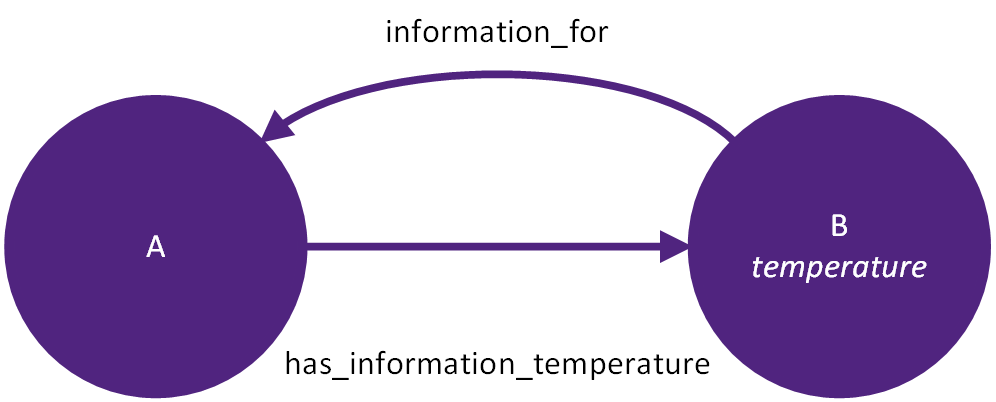
\includegraphics[width=8cm]{../../Images/04_Contribution/04_DDP_Inference.png}
  \caption{An example in which individual $A$ is connected to individual $B$ by $has\_information\_temperature$. We set the range of $has\_in{\f}ormation\_temperature$ to the class $Temperature$. As a result, the reasoner infers that $B$ must be of type $Temperature$.}
  \label{fig:04_DDP_Inference}
\end{figure}

\paragraph{Inconsistency}
We guard the consistency of the ontology using $DisjointClasses$. The $agrees\_with$ and $disagrees\_with$ object properties of the consensus and conflict patterns are naturally disjoint: when evidence $A$ agrees with evidence $B$, they cannot disagree at the same time. The decision design pattern inherits other inconsistency prevention mechanics from the completeness, reproducibility, consensus, and conflict patterns.

\paragraph{Generic ontology design pattern} \label{dop-godp}
The decision ontology pattern instantiates the completeness, reproducibility, consensus, and conflict patterns. These patterns have an overlap in their instantiation; for example, the consensus and conflict pattern both instantiate the $Reproducibility\_Base$. We reduce the overlap by defining new instantiation code. Code sample \ref{GODP_DDP_Instantiation_Basic} presents the instantiation code for the base ontology structure. The base instantiation code addresses the reproducibility, consensus, conflict, and a part of the completeness pattern. The base instantiation does not use any parameters.

\begin{lstlisting}[float,language=GDOL,caption={The base GDOL instantiation code for the decision ontology pattern. The instantiation code is a combination of the completeness, reproducibility, consensus, and conflict patterns.},label={GODP_DDP_Instantiation_Basic}][H]
pattern DecisionOntologyPattern_Basic = Reproducibility_Basic then
 %% Consensus pattern without reproducibility pattern
 ObjectProperty: agrees_with Domain: Evidence Range: Evidence Characteristics: Transitive, Symmetric
 ObjectProperty: based_on_evidence SuperPropertyOf: based_on_evidence o agrees_with SubPropertyOf: based_on_evidence
 %% Conflict pattern without reproducibility pattern
 ObjectProperty: disagrees_with Domain: Evidence Range: Evidence Characteristics: Symmetric, Irreflexive
 ObjectProperty: conflict_with_evidence SuperPropertyOf: based_on_evidence o disagrees_with SubPropertyOf: conflict_with_evidence
 %% Completeness pattern
 Completeness_dp [data_value][Information][xsd:int] %% Data property and information class as parameters
 Completeness_dp [data_description][Information][xsd:string] %% Data property and information class as parameters
 %% Used information
 Object Property: information_of InverseOf: has_information
 Class: Used_Information EquivalentTo: information_of some owl:Thing
 %% Used evidence
 Object Property: evidence_used_for InverseOf: based_on_evidence
 Class: Used_Evidence EquivalentTo: evidence_used_for some Information 
\end{lstlisting}
 
Figure \ref{fig:DecisionDesignPattern} presents the instantiated decision ontology pattern. This ontology does not include context. We took the \textcolor{Violet}{violet} edges and nodes from the evidence-based management pattern, the \textcolor{DarkBlue}{blue} edges and nodes from the reproducibility pattern, the \textcolor{Red}{red} edges from the conflict pattern, and the \textcolor{Green}{green} edge from the consensus pattern. The completeness pattern does not include structural elements.
 
\begin{figure}[H]
\centering
  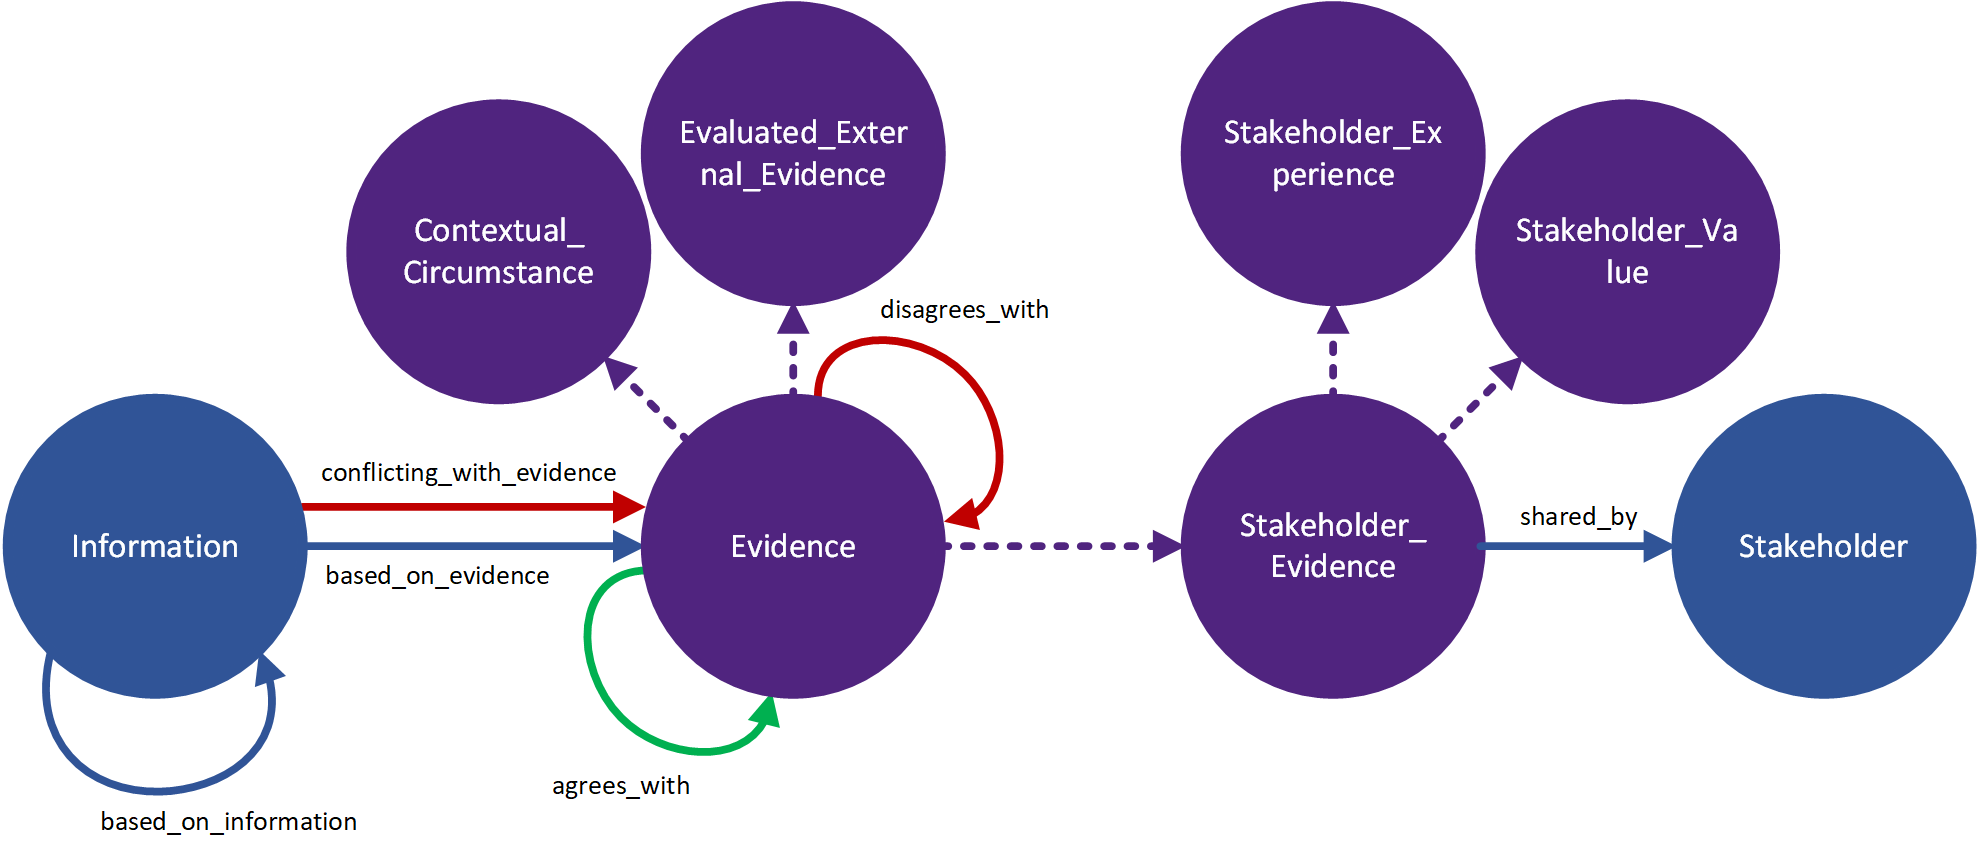
\includegraphics[width=15cm]{../../Images/04_Contribution/04_DecisionDesignPattern.png}
  \caption{The instantiated decision ontology pattern without context. We took the \textcolor{Violet}{violet} edges and nodes from the evidence-based management pattern, the \textcolor{DarkBlue}{blue} edges and nodes from the reproducibility pattern, the \textcolor{Red}{red} edges from the conflict pattern, and the \textcolor{Green}{green} edge from the consensus pattern.}
  \label{fig:DecisionDesignPattern}
\end{figure}

The completeness and reproducibility patterns require a context-specific instantiation. We instantiate a new context-specific ontology structure for every information type that decision-makers use to make a decision. We use parameter $i$ to represent this class. Code sample \ref{GODP_DDP_Instantiation_Context} presents the context-specific instantiation code. 

\begin{lstlisting}[float,language=GDOL,caption={The context-specific GDOL instantiation code to instantiate the decision design pattern. The code is a combination of the context-specific instantiation code of the completeness and reproducibility patterns.},label={GODP_DDP_Instantiation_Context}][H]
pattern DecisionOntologyPattern_Context [Class: i; Class: r] = 
 Completeness_op[has_information[i]; r; i] %% Object property, root class, and information class as parameters
\end{lstlisting}

\paragraph{Constraints}
We need to combine the basic and context-dependent constraints of the completeness, reproducibility, consensus, and conflict patterns. The constraints of the reproducibility and conflict patterns target the $Used\_In{\f}ormation$ class. Code sample \ref{SHACL_DDP_Basic} combines the constraints for these two patterns into one SHACL shape. 

\begin{lstlisting}[float,language=SHACL,caption={This code sample combines the constraints of the reproducibility, consensus, and conflict patterns. We have merged parts of the reproducibility and consensus patterns.},label={SHACL_DDP_Basic}][H]
UsedInformationShape a sh:NodeShape;
	sh:targetClass Used_Information; 
	sh:property [
		sh:or (
			[sh:path based_on_information; sh:minCount 1;]
			[sh:path based_on_evidence; sh:minCount 1;]
		)
		sh:severity sh:Violation; 
		sh:minCount 1; 
		sh:message "Reproducibility: increase the number of evidence sources for this information."; ];
	sh:targetClass Information; 
	# Conflict pattern
	sh:property [
		sh:path conflict_with_evidence; 
		sh:severity sh:Violation; 
		sh:maxCount 0; 
		sh:message "Conflict detected. Please resolve the conflict or re-consider using this information."; ];
\end{lstlisting}

Code sample \ref{SHACL_REP_SH} is part of the reproducibility pattern and presents the constraints that validate if $Stakeholder\_Evidence$ is $shared\_by$ a stakeholder. Code sample \ref{SHACL_CON_LEV} presents the constraints that validate the consensus pattern. We include both code samples as-is into the decision ontology pattern.

We instantiate the contextual constraints multiple times per scenario, depending on the need of the scenario. The completeness pattern is context-sensitive. Code sample \ref{SHACL_COM_DP} presents the only context-sensitive constraints we use in the decision design pattern.
\subsection{Decision presentation pattern} \label{odp_decision_presentation}
The outcome of a decision might deviate from the expectations of the decision-maker when the information maturity-level is low. This deviation is not a big problem when the impact of the decision on the organisation is low. However, when the impact of the decision on the organisation is high, the decision-maker wants more certainty that the decision reaches the expected outcome. There is a consensus on the benefits of evidence-based decision-making. However, \cite{DM03} and \cite{DM07} also raise the need for more research to prove its effectiveness.

\begin{center}
\large\color{document}{The decision presentation pattern helps decision-makers to make evidence-based decisions by presenting the information maturity-level.} 
\end{center}

The decision presentation pattern achieves this goal by enabling the decision-maker to understand the maturity-level of the decision-relevant information. We give decision-makers two options when we present the information maturity-level:
\begin{enumerate}
\item Accept the status of the decision-relevant information.
\item Elaborate further on the decision-relevant information.
\end{enumerate}

We enable the decision-maker to understand which information requires more elaboration. This elaboration can increase the completeness and reliability of the information. We present three dashboards for the decision-maker. The first dashboard presents the information maturity-level and evidence spread for all the decision-relevant information. The second dashboard presents the information maturity-level for the completeness, reproducibility, consensus, and conflict patterns. The third dashboard presents the maturity-levels per individual. 

Figure \ref{fig:04_Presentation_Components} presents a navigation concept for the three dashboards. The decision-maker can browse from the first dashboard to the second dashboard, from the second dashboard to the third dashboard, and from the first dashboard to the third dashboard. The context of the third dashboard changes depending on the origin of the decision-maker. For example, if the decision-maker browses from dashboard two to dashboard three using the completeness maturity-level, dashboard three presents the completeness of the decision-relevant information per individual.

\begin{figure}[H]
\centering
  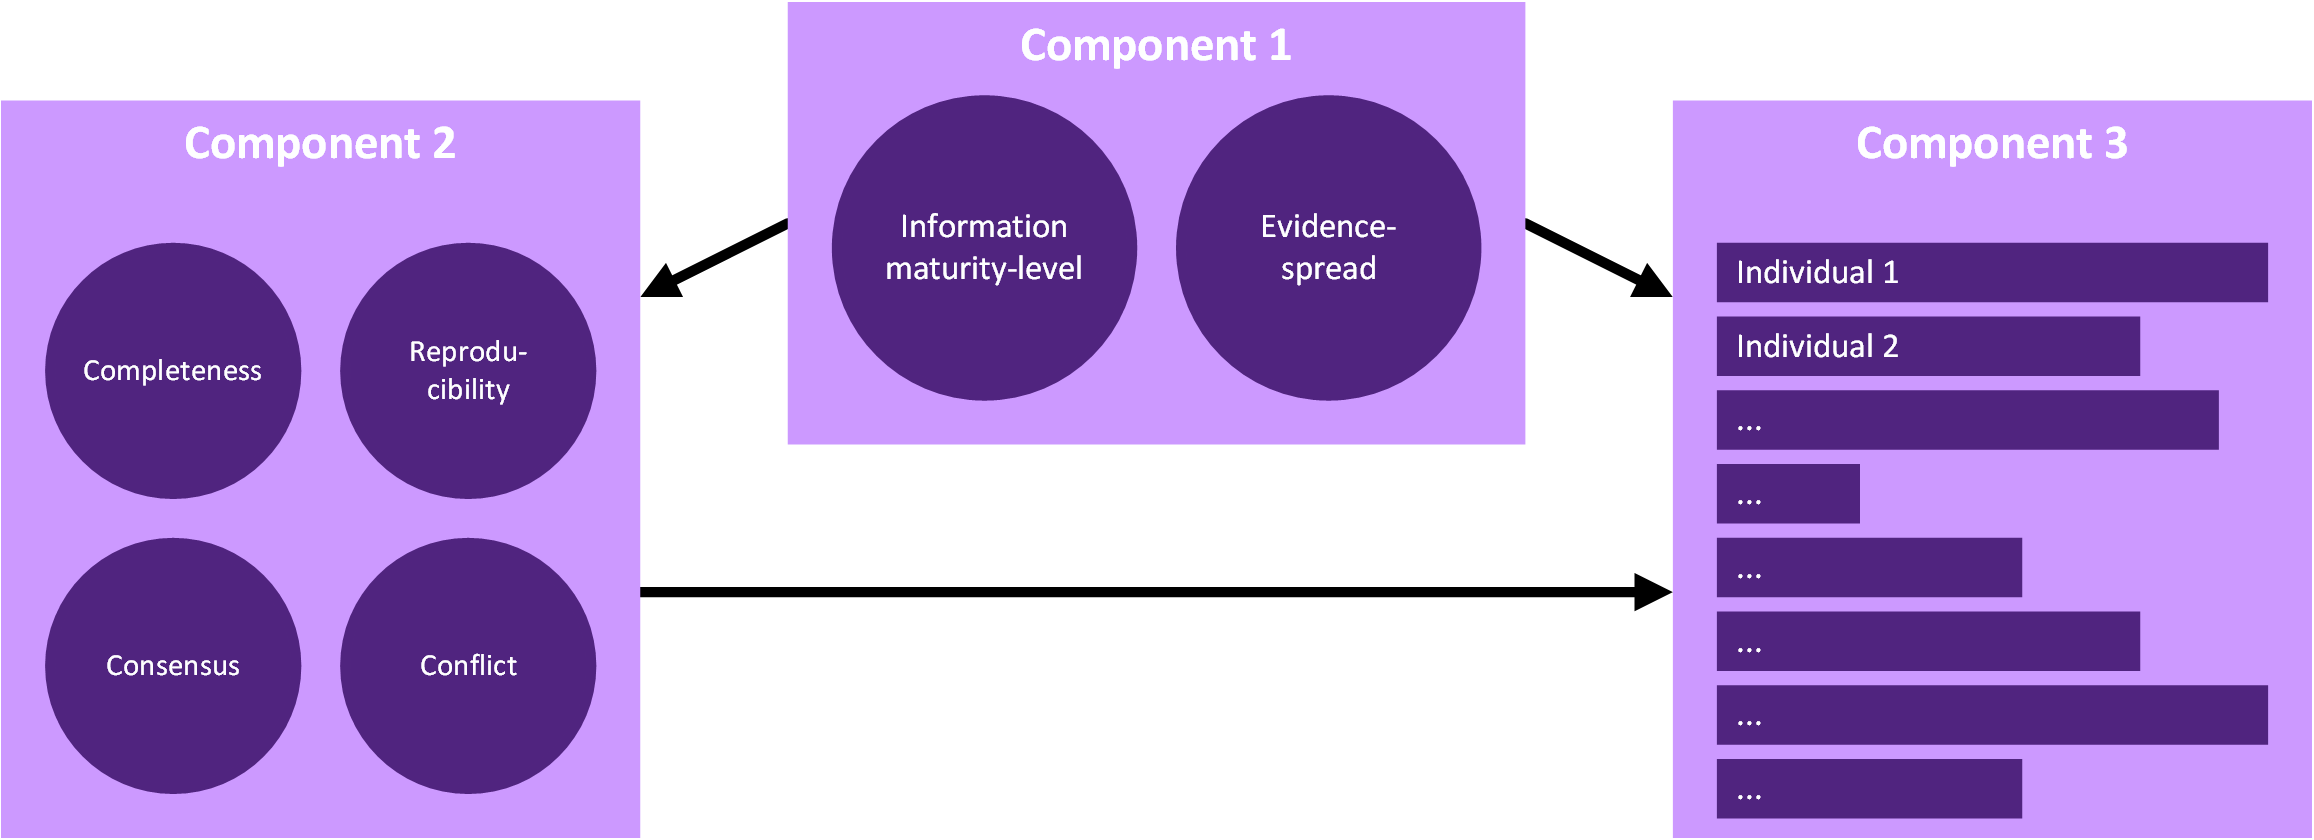
\includegraphics[width=16cm]{../../Images/04_Contribution/04_Presentation_Components.png}
  \caption{The three presentation dashboards that allow a decision-maker to understand the information-maturity level and evidence-spread.}
  \label{fig:04_Presentation_Components}
\end{figure} 

\subsubsection{Dashboard 1: Consolidated information maturity-level and evidence spread} \label{odp_maturity_evidence_spread}
The goal of the first dashboard is to help decision-makers to decide if the information maturity-level and evidence-spread are acceptable in the context of the specific decision. We determine an average information maturity-level and evidence-spread across the decision-relevant root individuals. Figure \ref{fig:root_information_target_1} repeats the definition of the root, information, and target individuals.

\begin{figure}[H]
\centering
  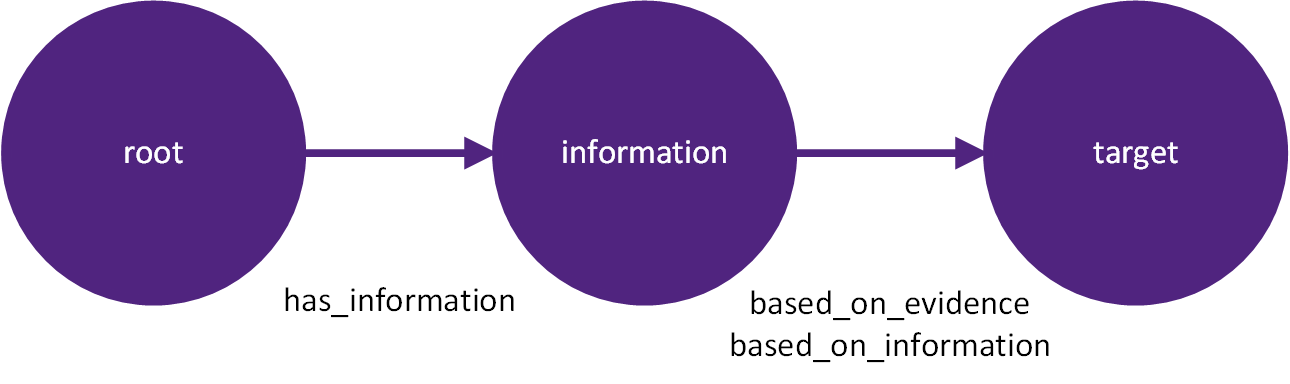
\includegraphics[width=10cm]{../../Images/04_Contribution/04_root_information_target.png}
  \caption{The $root$, $in{\f}ormation$, and $target$ individuals in n-ary relation.}
  \label{fig:root_information_target_1}
\end{figure}

We need to know the maximum number of violations before we can determine the information maturity-level. The maximum number of violations depends on the decision-relevant root individuals. We create a set $RI$ that contains the decision-relevant root individuals. The contents of the set $RI$ depend on the context of the decision. Therefore, we cannot define $RI$ as part of the pattern.  

\paragraph{Maximum number of violations: Completeness}
The maximum number of violations for the completeness pattern for a specific decision-relevant root individual depends on three things: 
\begin{enumerate}
\item The required $has\_in{\f}ormation\_*$ object properties.
\item The availability of the $data\_value$ and $data\_description$ data properties.
\item The availability of context-specific data properties.  
\end{enumerate}

First, we need to retrieve the $has\_in{\f}ormation\_*$ object properties for a specific decision-relevant root individual independent from the ontology content. We need to extract this information manually from the ontology structure by analysing the $has\_in{\f}ormation\_*$ object properties. We represent this manual extraction process in the function $hi(ri) \Rightarrow \mathbb{N}$. $ri$ represents a decision-relevant root individual.

Second, each $has\_in{\f}ormation\_*$ object property leads us to an individual classified as $Information$. Information individuals require a $data\_value$ and $data\_description$. Therefore, we multiply the output of $hi$ by $2$ and add it to the result. 

Third, adding additional object or data properties to the maximum number of violations for the completeness pattern might be necessary. We use variable $c$ for adding the context-specific violations for each decision-relevant root individual.

Equation \ref{eq:mvi1} returns the maximum number of violations for the completeness pattern considering the decision-relevant root individual $ri$ as a parameter: $mvi_1(ri) \rightarrow \mathbb{N}$.

\begin{equation} \label{eq:mvi1}
mvi_1(ri) = hi(ri) + 2hi(ri) + c
\end{equation}

Equation \ref{eq:mv_1} presents the maximum number of violations for the completeness pattern $mv_1$, considering the set of decision-relevant root individuals $RI$. The decision-relevant root individuals are context-dependent. We define a SPARQL query to extract the decision-relevant root individual per scenario.  

\begin{equation} \label{eq:mv_1}
mv_1(RI) = \sum_{ri \in RI} mvi_1(ri)
\end{equation}

\paragraph{Maximum number of violations: Reproducibility}
The maximum number of violations for the reproducibility pattern depends on the number of information classes that require reproduction. We use the same concept to retrieve the maximum number of violations for the reproducibility as we did for the completeness pattern. 

Equation \ref{eq:mvi2} returns the maximum number of violations for the reproducibility pattern considering the decision-relevant root individual $ri$ as a parameter: $mvi_2(ri) \rightarrow \mathbb{N}$.

\begin{equation} \label{eq:mvi2}
mvi_2(ri) = hi(ri)
\end{equation}

Equation \ref{eq:mv_2} presents the maximum number of violations $mv_2$ for the reproducibility pattern considering the set of decision-relevant root individuals $RI$. 

\begin{equation} \label{eq:mv_2}
mv_2(RI) = \sum_{ri \in RI} mvi_2(ri)
\end{equation}

\paragraph{Maximum number of violations: Consensus}
The maximum number of violations for the consensus pattern depends on the maximum number of used evidence sources in the context of a decision. Each evidence source can generate  one violation. Code sample \ref{SPARQL_CONS_IML_ri} presents a SPARQL query that counts the $Used\_Evidence$ individuals based on the object property $evidence\_used\_for$. $evidence\_used\_for$ is the inverse of $based\_on\_evidence$. 

\begin{lstlisting}[float,language=SPARQL1,caption={The SPARQL query that retrieves the number of individuals that the reasoner classified as $Used\_Evidence$ in the context of a specific root class.},label={SPARQL_CONS_IML_ri}][H]
SELECT (COUNT(DISTINCT ?t) as ?count) 
WHERE 
{
	?r has_information ?i .
	?i based_on_evidence ?t .
	?t rdf:type Used_Evidence .
	FILTER (?r = <ri_1>)
}
\end{lstlisting}

Equation \ref{eq:mvi2} returns the maximum number of violations for the reproducibility pattern considering the decision-relevant root individual $ri$ as a parameter: $mvi_3(ri) \rightarrow \mathbb{N}$. Function $uei(ri) \rightarrow \mathbb{N}$ represents the output of the SPARQL query code sample \ref{SPARQL_CONS_IML_ri} presents.

\begin{equation} \label{eq:mvi3}
mvi_3(ri) = uei(ri)
\end{equation}

We cannot sum the results of the individual violations as there might be duplicates in the results. For example, two information individuals might use the same evidence. When counting the maximum number of violations per individual, the sum would count this evidence as two violations. However, considering one decision, one evidence source can generate up to one violation. Code sample \ref{SPARQL_CONS_IML_RI} presents a new filter that we apply on code sample \ref{SPARQL_CONS_IML_ri}. We add the entire content of the set $RI$ to the filter. This way, we ensure that we get a list of evidence sources that is distinct for the specific decision.

\begin{lstlisting}[float,language=SPARQL1,caption={A new filter that we apply on code sample \ref{SPARQL_CONS_IML_ri}. We add the entire content of the set $RI$ to the filter.},label={SPARQL_CONS_IML_RI}][H]
FILTER (?r = <ri_1> || ?r = <ri_2> || ?r = <ri_x>)
\end{lstlisting}

Equation \ref{eq:mv_3} presents the maximum number of violations $mv_3$ for the reproducibility pattern considering the set of decision-relevant root individuals $RI$. Function $ue(RI) \rightarrow \mathbb{N}$ represents the SPARQL query code sample \ref{SPARQL_CONS_IML_RI} presents.

\begin{equation} \label{eq:mv_3}
mv_3(RI) = ue(RI)
\end{equation}

\paragraph{Maximum number of violations: Conflict}
The conflict pattern detects information individuals that have conflicting evidence using the $conflict\_with\_evidence$ object property. The pattern does not care about the number of conflicting evidence related to an individual. Alternatively, we could have used a similar mechanism as we used for the consensus pattern and detect conflict based on the $disagrees\_with$ object property. However, we solve the violation in the consensus pattern by adding an $agrees\_with$ object property to the evidence. The decision-maker can solve the conflict detected by the pattern by removing conflicting evidence or changing the information. In other words, the consensus pattern uses the $Evidence$ class as the core of the solution, while the conflict pattern uses the $Information$ class as the core of the solution.

The maximum number of conflict violations for a decision-relevant root individual depends on the maximum number of information classes that can be evidence-based. We re-use equation $mvi_2$ to determine the maximum number of conflict violations. Equation \ref{eq:mvi24} presents the maximum number of violations $mvi_4$ for the conflict pattern. 

\begin{equation} \label{eq:mvi24}
mvi_2(ri) = mvi_4(ri) = hi(ri)
\end{equation}

Equation \ref{eq:mv_4} presents the maximum number of violations $mv_4$ for the reproducibility pattern considering the set of decision-relevant root individuals $RI$. $mv_4$ is equal to $mv_2$.

\begin{equation} \label{eq:mv_4}
mv_4(RI) = \sum_{ri \in RI} mvi_4(ri)
\end{equation}

\paragraph{Consolidated information maturity-level}
We calculate the information maturity-level using the number of violations detected on the decision-relevant information and the maximum violations. For example, if an individual requires ten object properties and two data properties to be complete, and it triggers two violations, we define the information maturity-level as $(12-2)/12 = 83\%$. Equation \ref{eq:information_maturity_level} includes function $mv(RI) \Rightarrow \mathbb{N}$. This function calculates the maximum number of violations for the set of decision-relevant information. $av(RI) \Rightarrow \mathbb{N}$ calculates the actual number of violations for the set of decision-relevant information and $iml(RI) \Rightarrow \mathbb{N}$ represents the information maturity-level for the set.

\begin{equation} \label{eq:information_maturity_level}
iml(RI) = \dfrac{mv(RI)-av(RI)}{mv(RI)}
\end{equation}

We can easily retrieve the actual number of violations from, for example, Prot\'eg\'e and the SHACL4P plugin. Figure \ref{fig:04_Presentation_IML_SHACL4P} presents an example for which the defined constraints detected two violations for $Opportunity\_SC2\_Vision\_Contribution$. 

\begin{figure}[H]
\centering
  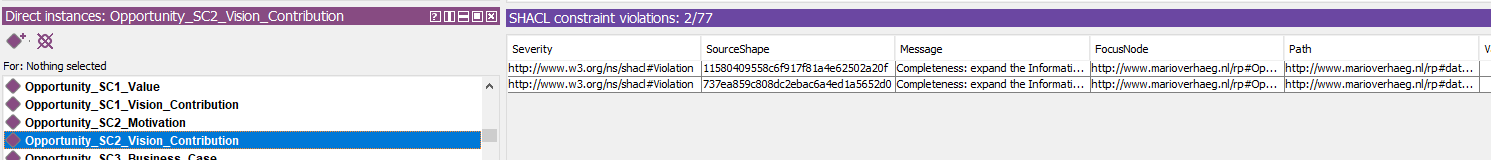
\includegraphics[width=17cm]{../../Images/04_Contribution/04_Presentation_IML_SHACL4P.png}
  \caption{The constraints detect two violations for $Opportunity\_SC2\_Vision\_Contribution$ in Prot\'eg\'e.}
  \label{fig:04_Presentation_IML_SHACL4P}
\end{figure}

Additionally, we need to define the maximum number of violations per decision-relevant root individual and pattern. The maximum number of violations per pattern for a specific individual defines the total maximum number of violations: $mv(RI) = mv_1(RI) + mv_2(RI) + mv_3(RI) + mv_4(RI)$, in which:
\begin{enumerate}
\item $mv_1(RI)$ is the maximum number of violations for the completeness pattern.
\item $mv_2(RI)$ is the maximum number of violations for the reproducibility pattern.
\item $mv_3(RI)$ is the maximum number of violations for the consensus pattern.
\item $mv_4(RI)$ is the maximum number of violations for the conflict pattern
\end{enumerate}

$RI$ represents the set of decision-relevant root individuals.

\paragraph{Evidence spread}
We increase the transparency of the information maturity-level by presenting the evidence spread. For example, a decision entirely based on the evidence type $Stakeholder\_Experience$ might require more elaboration. We use a query to extract the evidence spread from the decision ontology pattern. Within this query, we search for root individuals $ri$ that represent decision-relevant information. The filter in the query accepts multiple root individuals using $||$ the (OR) filter criteria. Code sample \ref{SPARQL_ES} presents the SPARQL query. 

\begin{lstlisting}[float,language=SPARQL1,caption={The SPARQL query that retrieves the evidence spread for decision-relevant information. The SPARQL query counts the individuals that are based on a specific evidence class using type $?t$ of evidence class $?e$.},label={SPARQL_ES}][H]
SELECT ?t (COUNT(DISTINCT ?t) as ?count) 
WHERE 
{
	{
			?ri has_information ?i .
    		?i based_on_evidence ?e .
    		?e rdf:type ?t .
	}
	FILTER(?ri = <ri1> || ?ri = <ri2> || ?rix = <rix> ).
	FILTER(?t != owl:Thing && ?t != Evidence && ?t != Used_Evidence && ?t != Stakeholder_Evidence)
}
GROUP BY ?t
\end{lstlisting}

\paragraph{Overview dashboard}
The goal of the first high-level dashboard is to help the decision-maker answering the question:

\begin{center}
\large\color{document}{Is the information ready for an evidence-based decision?}
\end{center}

This dashboard consists of two charts: the overall information maturity-level and the evidence spread. The information maturity-level helps the decision-maker to understand the quality-level of the information related to this decision. The evidence-spread helps the decision-maker to understand the source of the evidence. The decision-maker needs to find a balance between the information maturity-level and the decision impact, and the evidence-spread and the decision impact. When the impact of a decision is relatively low, the decision-maker might accept a lower information maturity-level and a consolidated evidence-spread. However, when the impact of a decision is relatively high, we expect that decision-makers will require a higher information maturity-level and would like to see a dispersed evidence-spread.

We use a pie-chart to help the decision-maker to understand the mix of evidence-types. The pie-chart is suitable to present relative proportions and percentages \parencite{OTH09}.

We express the information maturity-level as a percentage. Therefore, we use a pie-chart for presenting the information maturity-level as well. Figure \ref{fig:Dashboard_Component_1} presents an example of a dashboard that contains the pie chart presenting the evidence-spread and the information maturity-level. We shorten the time it takes for a decision-maker to consume the information on the dashboard by limiting the number of charts, using data labels to show the actual values, and using a clear legend \parencite{BI09}. Additionally, we use an analogous colour scheme for the evidence spread to ensure the chart appears as one, but the colours are still easily recognisable \parencite{BI10}. The pie chart presenting the information maturity-level uses a different colour scheme, representing \emph{good} (the mature information) and \emph{bad} (the premature information) as \textcolor{LightGreen}{green} and \textcolor{Red}{red}.

\begin{figure}[H]
\centering
  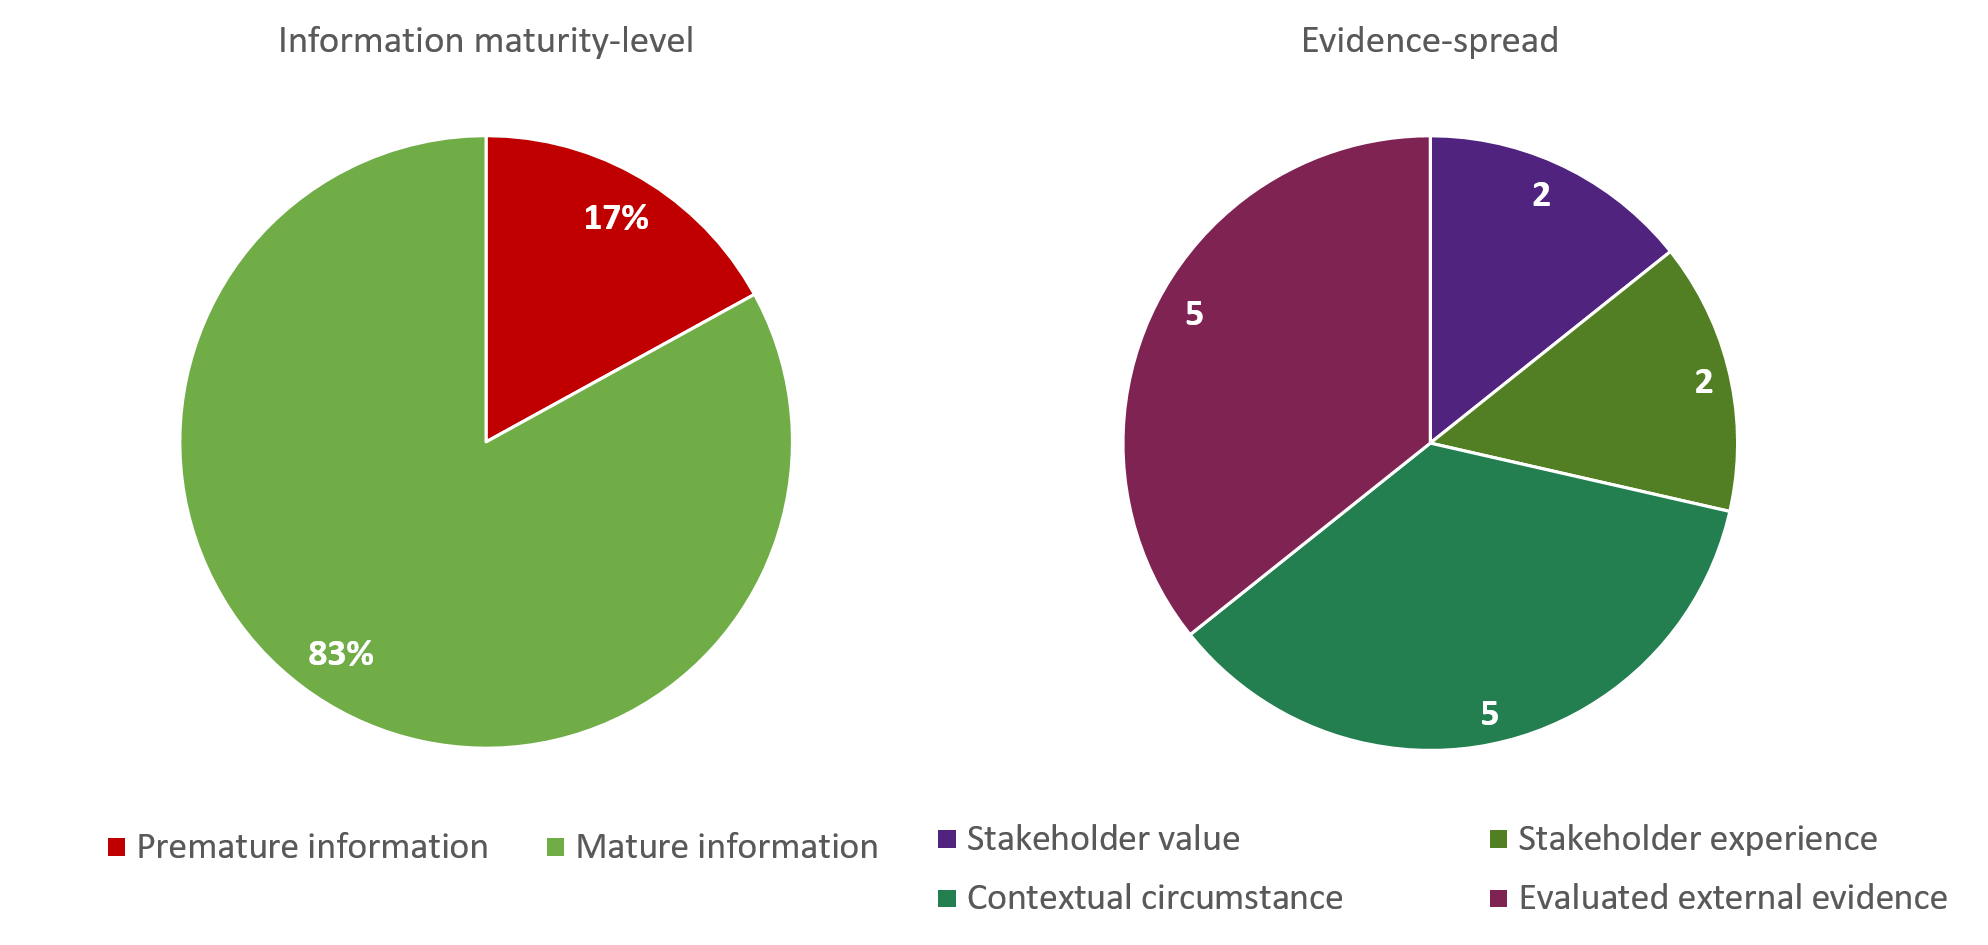
\includegraphics[width=14cm]{../../Images/04_Contribution/Dashboard_Component_1.png}
  \caption{A mock-up of the presentation of the evidence-mix of a specific decision.}
  \label{fig:Dashboard_Component_1}
\end{figure} 

The decision-maker can navigate to the second dashboard by clicking on the pie chart that presents the information maturity-level. Alternatively, the decision-maker can navigate to the third dashboard by clicking on the pie chart that presents the evidence-spread.

\subsubsection{Dashboard 2: Information maturity-level in detail}
The goal of the second dashboard is to enable a decision-maker to understand the consolidated information maturity-level. If the consolidated information maturity-level is lower than expected, the decision-maker can use the second dashboard to understand the root cause. This understanding allows the decision-maker to define actions to improve the information maturity-level. For example, the decision-maker needs to spend time on expanding the information if the completeness pattern causes a low information maturity-level. However, the decision-maker should understand the conflicts and reconsider using conflicting evidence sources if these evidence sources cause a low information maturity-level.

\paragraph{Pattern information maturity-levels}
The detailed information maturity-level consist out of the maturity-level for the completeness, reproducibility, consensus, and conflict patterns. We have defined the functions $mv_1$, $mv_2$, $mv_3$, and $mv_4$ for this. 

In addition to the actual violations $av$, we define $av_1(RI) \Rightarrow \mathbb{N}$, $av_2(RI) \Rightarrow \mathbb{N}$, $av_3(RI) \Rightarrow \mathbb{N}$, and $av_4(RI) \Rightarrow \mathbb{N}$ to represent the actual violations for the completeness, reproducibility, consensus, and conflict patterns. We also define the $avi_x(ri)$ functions that represent the actual violations that a decision-relevant individual generates. Equation \ref{eq:information_maturity_level_x} presents the information maturity-level of the decision-relevant root individuals $RI$ for one of the patterns.

\begin{equation} \label{eq:information_maturity_level_x}
iml_x(RI) = \dfrac{mv_x(RI)-av_x(RI)}{mv_x(RI)}
\end{equation}

\paragraph{Detailed information maturity-level dashboard}
Equation \ref{eq:information_maturity_level_x} defines four pattern-specific information maturity-levels. The pie-chart is most suitable to present percentages and relative proportions \parencite{OTH09}. Figure \ref{fig:Dashboard_Component_2} presents an example of a dashboard that contains the pie charts that present the pattern-specific information maturity-levels. We have made the pie charts easy to understand by tailoring the scales to the specific pattern, representing \emph{good} (the mature information) and \emph{bad} (the premature information) as \textcolor{LightGreen}{green} and \textcolor{Red}{red}, and using data labels. The decision-maker can navigate to the third dashboard by clicking on one of the pie charts. 

\begin{figure}[H]
\centering
  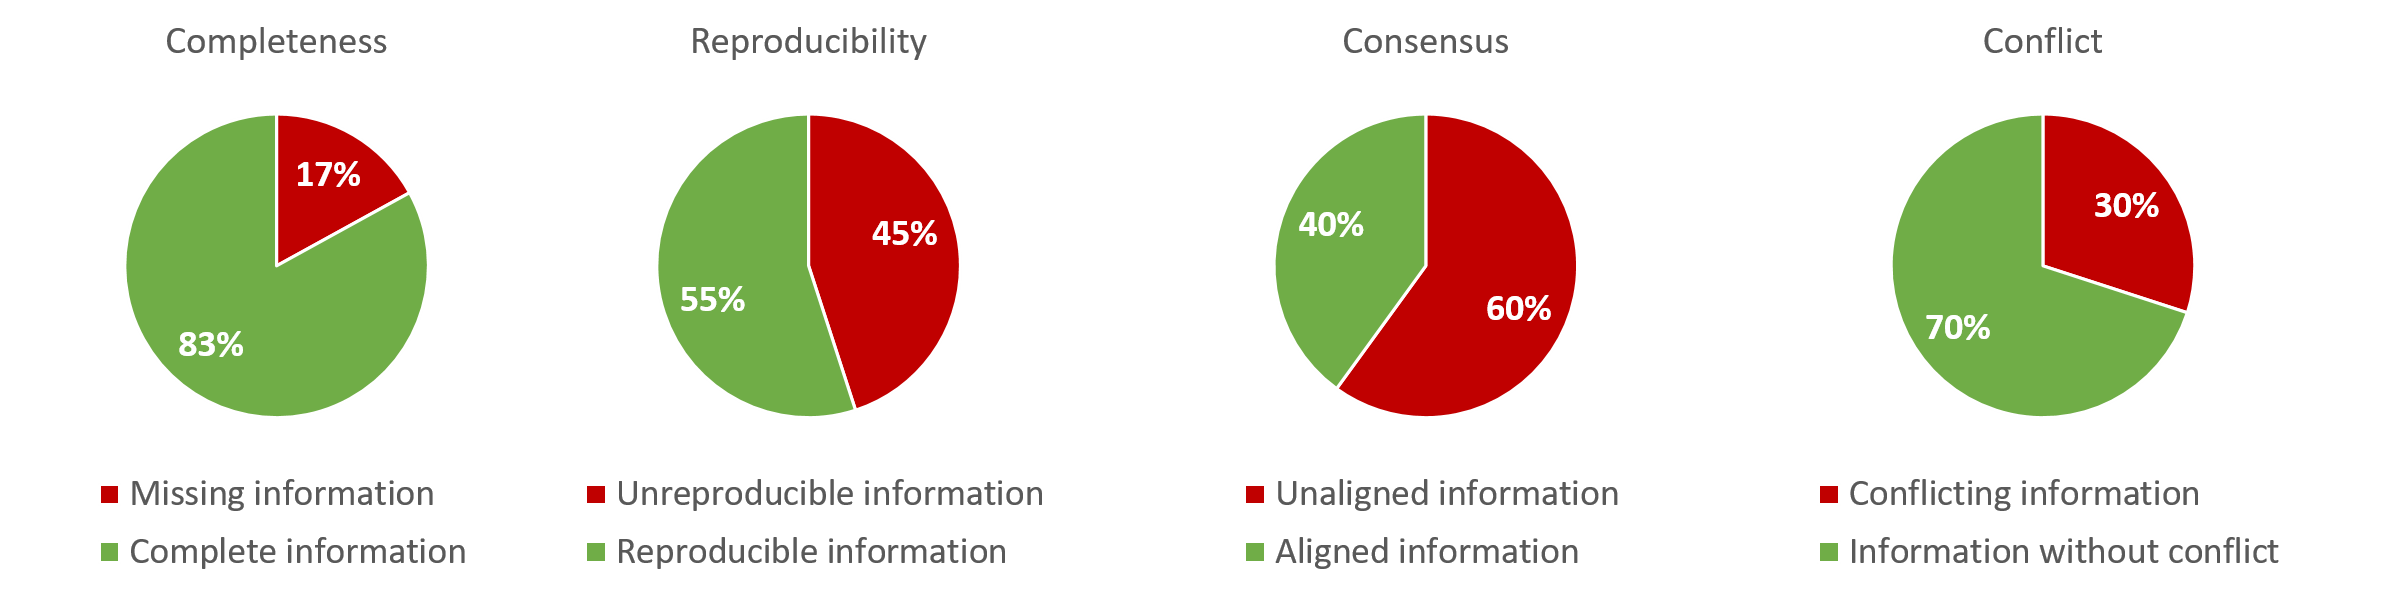
\includegraphics[width=17cm]{../../Images/04_Contribution/Dashboard_Component_2.png}
  \caption{A mock-up of the presentation of the pattern-specific information maturity-levels.}
  \label{fig:Dashboard_Component_2}
\end{figure} 

\subsubsection{Dashboard 3: Violations}
The goal of the third dashboard is to enable the decision-maker to understand which individuals cause the lowered information maturity-level and the evidence spread. The decision-maker might have the following questions:
\begin{enumerate}
\item How can I diversify the evidence types to increase the information maturity-level?
\item Which information is missing?
\item Which information is unreproducible or does not meet the consensus-level?
\item Which information has evidence conflicts?
\end{enumerate}

The answer to these questions allows the decision-maker to increase the information maturity-level. The decision-maker can complete information by entering new information, can reproduce information by linking it to existing or new evidence sources, or remove conflict by discarding information or replacing evidence sources. We focus on the data structure, detection mechanisms, and data presentation. Creating forms to enter new information or change existing information is, therefore, not in the scope of this study. 

We tailor the presentation of the third dashboard, depending on these four questions. The structure of the presented information is similar for the four use-cases. The level of detail requires us to present the information per individual. As a result, we need to present multiple individuals in the same environment. We only present premature individuals to prevent overwhelming the decision-maker with information. Presenting the mature individuals does not make it easier for the decision-maker to answer the questions mentioned earlier.

We want the decision-maker to see the difference between the categories of information in each of the four questions, for example, complete versus incomplete. Presenting the diversity of evidence types for multiple individuals requires four categories: evaluated external evidence, stakeholder value, stakeholder experience, and contextual circumstances. A bar chart allows the decision-maker to compare data across categories \parencite{OTH09}. 

\paragraph{Individual dashboard}
Figure \ref{fig:Dashboard_Component_3_Completeness} presents an example of the presentation of the completeness maturity-level of four individuals. We show the completeness maturity-level for each individual using a bar chart. The number of individuals depends on the scope of the decision. We present the related violations in a table below the bar chart for the selected decision. Even though entering or changing information is not in the scope of this study, we can easily imagine that clicking on one of the violations would direct the decision-maker to a form that allows the decision-maker to enter or adjust information and, as a result, solve the violation immediately. We use the same presentation for the reproducibility, consensus, and conflict-related questions. However, we replace the header of the chart and the name of the data series.

\begin{figure}[H]
\centering
  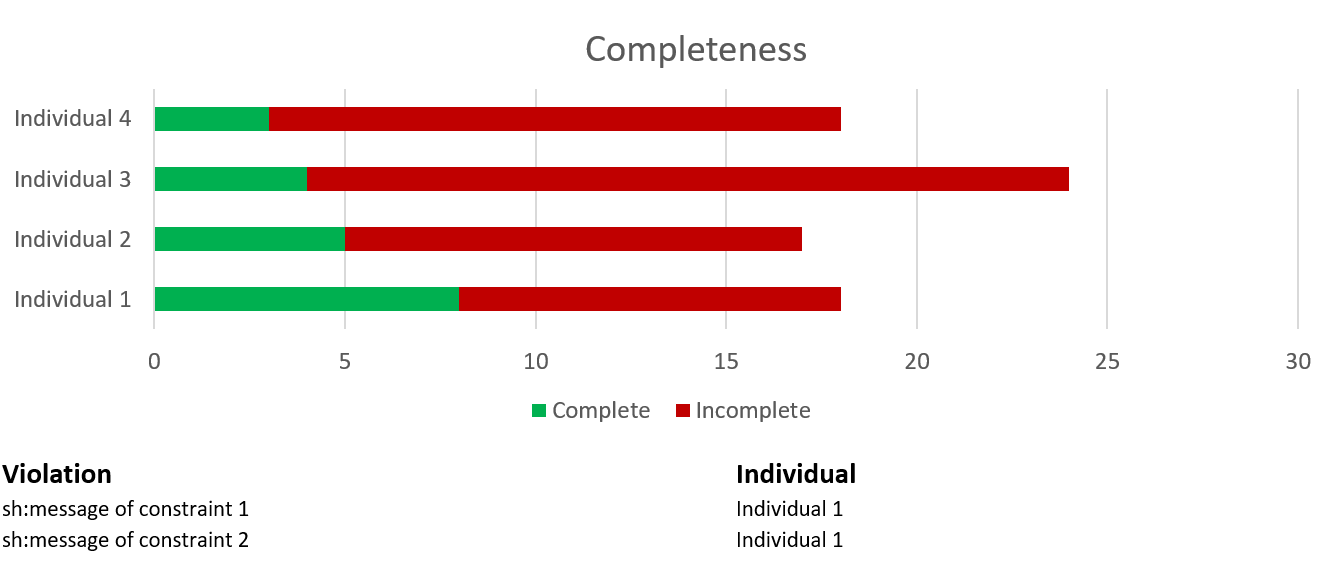
\includegraphics[width=16cm]{../../Images/04_Contribution/04_DecisionPresentationPattern_Component3_Example_Completeness.png}
  \caption{A mock-up of the presentation of the completeness maturity-level of four individuals. We show the completeness maturity-level for each individual using a bar chart.}
  \label{fig:Dashboard_Component_3_Completeness}
\end{figure} 

We extract the actual individual violations from the ontology. The $mvi_1$, $mvi_2$, $mvi_3$, and $mvi_4$ functions define the maximum number of violations per individual. We subtract the actual violations $av$ from the maximum violations $mv$ to get the information without conflict, the complete information, the reproducible information, and the aligned information.

\paragraph{Evidence spread dashboard}
The presentation of the evidence spread is a bit different. Instead of two data series, we need four data series: one for each evidence type. Figure \ref{fig:Dashboard_Component_3_Spread} presents an example of the presentation of the evidence spread of four individuals. We have chosen for a consistent colouring scheme, considering figure \ref{fig:Dashboard_Component_1}. We present the evidence spread for each individual using a bar chart. There are no constraints that enforce a specific evidence spread. Therefore, there are no violations to present. Instead, we present a list of evidence related to the selected individual below the bar chart. Furthermore, we consolidate the list of violations based on the root individuals. This presentation allows a decision-maker to understand the evidence spread and actual evidence related to a root individual. 

\begin{figure}[H]
\centering
  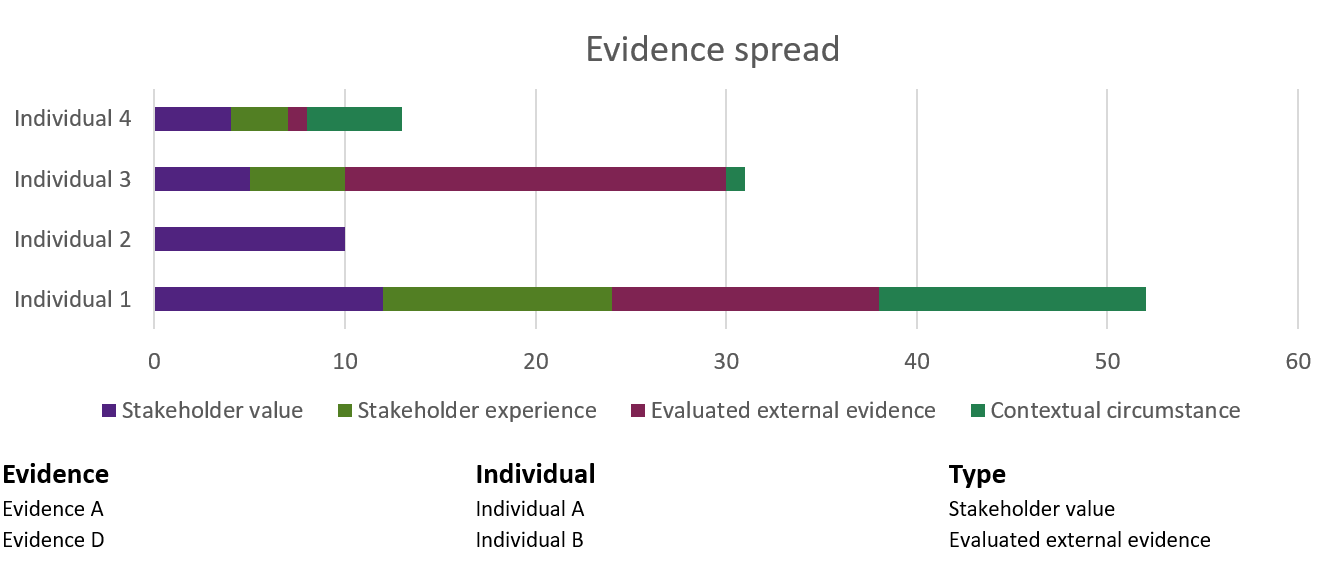
\includegraphics[width=16cm]{../../Images/04_Contribution/04_DecisionPresentationPattern_Component3_Example_Spread.png}
  \caption{A mock-up example of the presentation of the evidence spread of four individuals. We have chosen for a consistent colouring scheme, considering figure \ref{fig:Dashboard_Component_1}. We present the evidence spread for each individual using a bar chart.}
  \label{fig:Dashboard_Component_3_Spread}
\end{figure} 

We considered using an alternative presentation based on graphs. Figure \ref{fig:Dashboard_Component_3_Alternative} presents an example of this presentation. The graph-based presentation overwhelms the decision-maker with a lot of details, including the relationships between decision-relevant information and their status. This example presents only seven decision-relevant individuals. A more extensive example increases the size and complexity of the presentation. Additionally, the edges do not add useful information for the decision-maker.

\begin{figure}[H]
\centering
  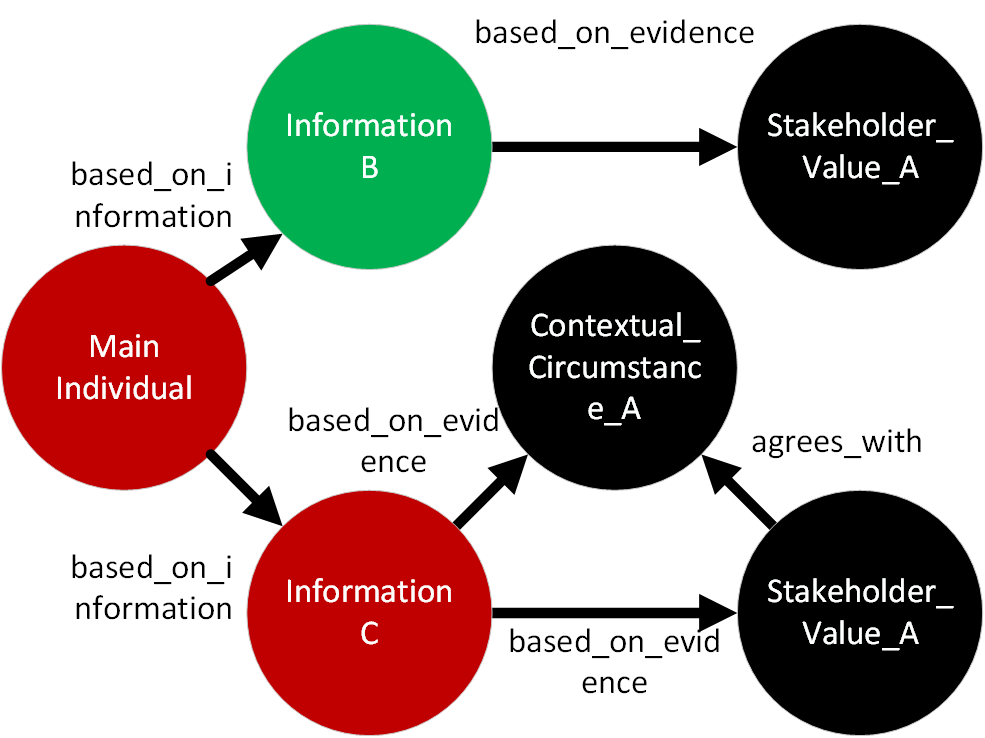
\includegraphics[width=7cm]{../../Images/04_Contribution/04_DecisionPresentationPattern_Component3_Example_Alternative.png}
  \caption{An alternative, more complex, presentation of the decision-relevant individuals and their maturity status.}
  \label{fig:Dashboard_Component_3_Alternative}
\end{figure} 

\section{Validation} \label{validation}
The decision ontology pattern consolidates the completeness, reproducibility, consensus, and conflict patterns. These patterns are useful on their own. However, only their consolidation, combined with the evidence-management pattern, contributes to the answer to our research question. Therefore, we validate the consolidated decision ontology pattern in this chapter. Additionally, we also validate the decision presentation pattern in this chapter. 

We use two scenarios to validate the decision ontology pattern and decision presentation pattern:
\begin{enumerate}
\item \nameref{val-rp}
\item \nameref{val-as}
\end{enumerate}

The goal of the first scenario is to prove the decision design pattern leads to the expected results. The goal of the second scenario is to prove that the decision design pattern can be applied in other scenarios as well. We limit the validation depth of the second scenario when there is an overlap with the first scenario. 

These scenarios are related to each other. A software product manager first prioritises the requirements in his backlog. Each requirement specifies a problem to solve or a goal to reach. Once the product team picks a requirement for implementation, the product team uses alternative solution selection to select the right technical solution to solve the specified problem or reach a specific goal. Both scenarios have challenges that attract the interest of academics. We use these scenarios as examples for which the decision design pattern increases the transparency of the information maturity-level. Software product managers can use this transparency to evaluate if the information is ready to make an evidence-based decision.

\subsection{Scenario 1: Requirements prioritisation} \label{val-rp}
The goal of the requirements prioritisation scenario is to validate if the decision design pattern can help software product managers to use evidence-based requirements prioritisation.

\begin{center}
\large\color{document}{\valone} 
\end{center}

A software product manager needs to decide if one requirement is more important than another requirement. The software product manager contributes to reaching the defined goals of the product when the software product manager puts the requirement on the right position in the backlog. These goals are, for example, related to the revenue of the product or the size of its user base. When the software product manager puts the requirement on a higher position in the backlog, then it is supposed to be, another requirement is on a lower position then it should be.

\subsubsection{Decision ontology pattern}
We base the definition of the decision ontology pattern for requirements prioritisation on section \ref{tf-val-rp} \nameref{tf-val-rp} of the theoretical framework. Table \ref{table:rp_formal_dataproperties} presents the knowledge criteria that a software product manager uses to decide which requirement, out of two, is most important. We define the $Requirement$ and $Insight$ (with sub-classes $Challenge$ and $Opportunity$) as decision-relevant \emph{root} classes. We need the $Vision$ class for the reproduction of information. Figure \ref{fig:rpp-ont} presents the ontology.  

\begin{figure}[H]
\centering
  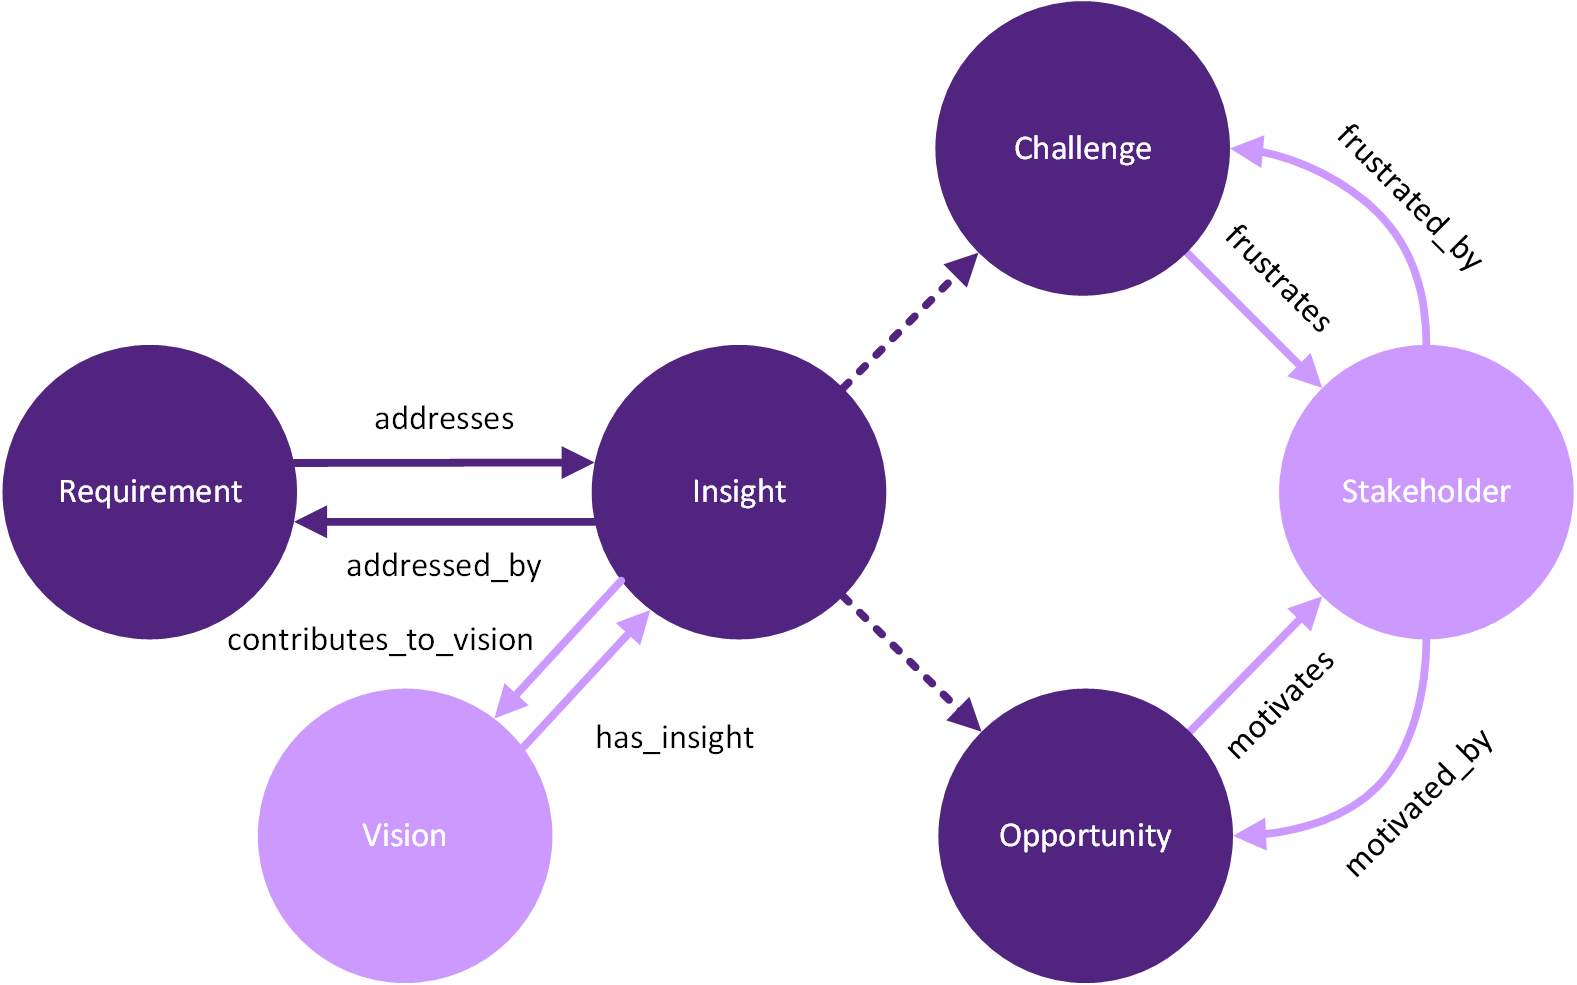
\includegraphics[width=12cm]{../../Images/05_Validation/05_ONT_RP.png}
  \caption{The requirements prioritisation ontology. The \textcolor{Violet}{violet} nodes represent the decision-relevant root classes. The \textcolor{LightViolet}{light violet} nodes represent the classes we need for the reproduction pattern.}
  \label{fig:rpp-ont}
\end{figure}

The $addresses$ and $contribute\_to\_vision$ object properties are essential for the structural integrity of the ontology. A $Requirement$ that does not address an $Insight$ and an $Insight$ that does not contribute to a $Vision$ are structural problems. Missing these object properties influences the reliability of the information that we present in the dashboards.

\subsubsection{Instantiation of the decision ontology pattern}
We instantiate the base decision ontology pattern once for the requirement prioritisation scenario. Code sample \ref{GODP_RP_INST_Basic} presents the instantiation of the base decision ontology pattern. We expand the decision ontology pattern with the ontology figure \ref{fig:rpp-ont} presents manually.

\begin{lstlisting}[float,language=GDOL,caption={The GDOL instantiation code of the basic instantiation of the decision design pattern.},label={GODP_RP_INST_Basic}][H]
Ontology RequirementsPrioritisation = DecisionOntologyPattern_Basic
\end{lstlisting}

The requirements prioritisation ontology and the instantiated decision design pattern include a $Stakeholder$ class. We manually merge the $Stakeholder$ classes from these ontologies into a single $Stakeholder$ class. Alternatively, we could have decided to define both that $Stakeholder$ classes are equal. However, merging the two $Stakeholder$ classes into one class reduces the number of classes and, therefore, reduces the complexity of the ontology.

The context-specific instantiation of the decision design pattern requires parameters to extend the ontology with a context-specific structure. We use the context-specific instantiation to, for example, instantiate the knowledge criteria in a way we can validate their completeness and reproducibility.

Table \ref{table:rp_formal_dataproperties} presents the knowledge criteria that a software product manager needs to understand to decide if one requirement is more important than another requirement. We add the knowledge criteria to the domain of the $Insight$ and $Requirement$ classes of the requirements prioritisation ontology. We define the completeness-level of a $Requirement$ and $Insight$ based on the knowledge criteria. 

\begin{table}[H]
\centering
\caption{An overview of the formal knowledge criteria that requirement prioritisation needs based on the description in section \ref{tf-val-rp} \nameref{tf-val-rp}. Code sample \ref{GODP_RP_INST_Knowledge_Criteria} instantiates the knowledge criteria.}
\begin{tabular}{| p{9cm} | p{4cm} | }
\hline
\rowcolor{document}
\color{documentText}Data Property & \color{documentText}Domain  \\
\hline
$insight\_value$ & $Addressed\_Insight$  \\
\hdashline
$insight\_vision\_contribution$ & $Addressed\_Insight$   \\
\hdashline
$insight\_reach$ & $Addressed\_Insight$  \\
\hdashline
$requirement\_insight\_contribution$ & $Requirement$   \\
\hdashline
$requirement\_value$ & $Requirement$   \\ 
\hdashline
$requirement\_cost$ & $Requirement$   \\ 
\hdashline
$requirement\_confidence$ & $Requirement$  \\ 
\hline
\end{tabular}
\label{table:rp_formal_dataproperties}
\end{table}

We instantiate each knowledge criteria using the generic ontology design pattern presented by code sample \ref{GODP_DDP_Instantiation_Context}. The generic ontology design pattern $DecisionDesignPattern\_Context$ uses two parameters: the information class and the decision-relevant root class. Code sample \ref{GODP_RP_INST_Knowledge_Criteria} presents, for example, the instantiation of the $insight\_value$ as an example. Code sample \ref{GODP_RP_INST_Knowledge_Criteria_Result} shows the instantiated generic ontology design pattern.

\begin{lstlisting}[float,language=GDOL,caption={The GDOL instantiation code of the knowledge criteria.},label={GODP_RP_INST_Knowledge_Criteria}][H]
DecisionOntologyPattern_Context[insight_value][Addressed_Insight]
\end{lstlisting}

\begin{lstlisting}[float,language=GDOL,caption={The result of the GDOL instantiation code that code sample \ref{GODP_RP_INST_Knowledge_Criteria} presents.},label={GODP_RP_INST_Knowledge_Criteria_Result}][H]
Completeness_op [has_information_insight_value][Addressed_Insight][insight_value] 
\end{lstlisting}

Code sample \ref{SHACL_RP_INST_Completeness} shows the instantiated SHACL shapes for, for example, the $insight\_value$. We need to adjust the $sh:targetClass$, $sh:path$, and $sh:message$ variables manually.

The constraints generate three violations when a knowledge criterion is not available. One violation represents the unavailability of the knowledge criterion itself, and the other two violations represent the missing $data\_value$ and $data\_description$. It is possible to add more violations if the context requires this.

\begin{lstlisting}[float,language=SHACL,caption={An example of instantiated SHACL shapes for the data property $insight\_value$. We instantiate this code sample for each knowledge criterion and for each information required to reproduce a knowledge criterion.},label={SHACL_RP_INST_Completeness}][H]
rp:Addressed_InsightShape a sh:NodeShape;
	sh:targetClass rp:Addressed_Insight; 
	sh:property [
		sh:path rp:has_information_insight_value;
		sh:severity sh:Violation; 
		sh:minCount 1; 
		sh:message "Completeness: add insight_value to the Addressed_Insight."; ];
	sh:property [
		sh:path rp:has_information_insight_value;
		sh:severity sh:Violation; 
		sh:minCount 1; 
		sh:message "Completeness: add data_value to the insight_value."; ];
	sh:property [
		sh:path rp:has_information_insight_value;
		sh:severity sh:Violation; 
		sh:minCount 1; 
		sh:message "Completeness: add data_description to the insight_value."; ];
\end{lstlisting}

The reproduction of knowledge criteria uses the completeness pattern. With the instantiation of the generic ontology design pattern and the constraints, we can validate the reproducibility of the knowledge criteria throughout the information chain figure \ref{fig:reproducibility_chain_val_rp} shows.

\begin{figure}[H]
\centering
  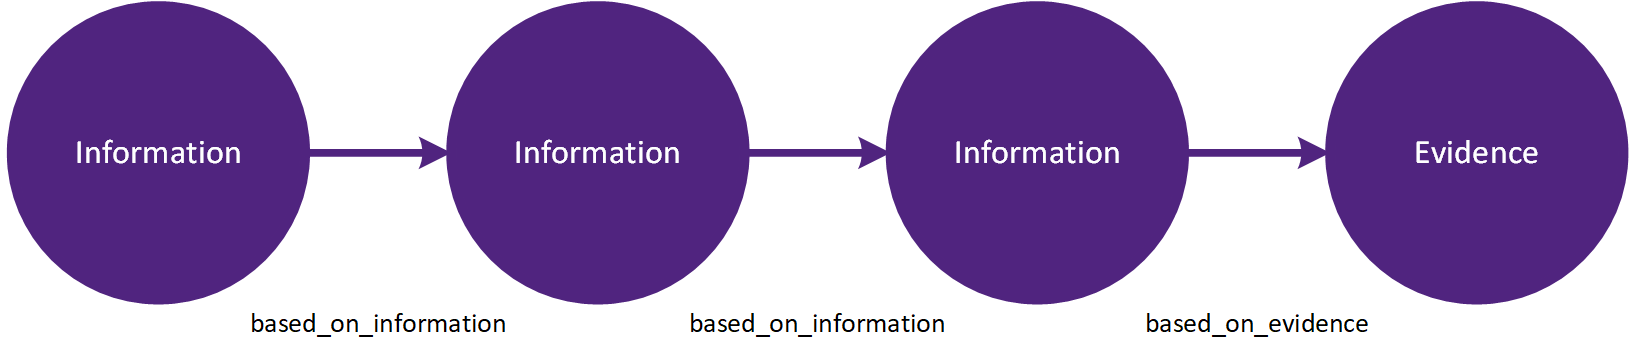
\includegraphics[width=12cm]{../../Images/Reproducibility_Chain.png}
  \caption{An example of an evidence-based chain of information. The reproducibility pattern should detect if the chain is not evidence-based.}
  \label{fig:reproducibility_chain_val_rp}
\end{figure} 

\paragraph{Insight value}
The insight value takes input from the stakeholder on the \emph{frustration} (challenge) or \emph{motivation} (opportunity) the stakeholder experiences. We consider a description of the \emph{business case} from the stakeholder's perspective as well. Table \ref{table:rpp_insight_value} presents an overview of the background information the software product manager requires to define the insight value.

\begin{table}[H]
\centering
\caption{The background information that we require to reproduce the value of an insight.}
\begin{tabular}{| p{3cm} | p{4cm} | p{8cm} | }
\hline
\rowcolor{document}
\color{documentText}$has\_in{\f}ormation\_*$ & \color{documentText}Class & \color{documentText}Description  \\
\hline
$challenge\_$ ${\f}rustration$ & $Addressed\_Challenge$ & The current pain the stakeholder experiences. A stakeholder finds this insight a necessary \emph{fix}. \\
\hdashline
$opportunity\_$ $motivation$ & $Addressed\_Opportunity$ & The motivation of a stakeholder to use the product more often if a requirement addresses this insight. \\
\hdashline
$insight\_$ $business\_case$ & $Addressed\_Insight$ & Increased revenue, decreased cost, or decreased business risk. \\
\hline
\end{tabular}
\label{table:rpp_insight_value}
\end{table}

Code sample \ref{GDOP_RP_INST_Insight_Value} presents the instantiation of the $Insight\_Value$. 

\begin{lstlisting}[float,language=GDOL,caption={The GDOL instantiation code of the information reproducing the $Insight\_Value$},label={GDOP_RP_INST_Insight_Value}][H]
DecisionDesignPattern_Context[challenge_frustration; Addressed_Challenge]
DecisionDesignPattern_Context[opportunity_motivation; Addressed_Opportunity] 
DecisionDesignPattern_Context[insight_business_case; Addressed_Insight]
\end{lstlisting}

\paragraph{Vision contribution}
The vision itself needs to be defined to validate if the insight contributes to the vision. We introduce the $Vision$ class for this. The vision class hosts the vision statement (and related time frame), a measurable objective (and related time frame), a current state and target condition. Table \ref{table:rp_vision_contribution} presents an overview of the background information the software product manager requires to define the vision contribution. 

\begin{table}[H]
\centering
\caption{The background information that we require to reproduce the vision contribution of an insight.}
\begin{tabular}{| p{3cm} | p{2cm} | p{10cm} | }
\hline
\rowcolor{document}
\color{documentText}$has\_in{\f}ormation\_*$ & \color{documentText}Class & \color{documentText}Description  \\
\hline
$vision\_$ $statement$ & $Used\_Vision$ & A futuristic goal defined in the context of a product or company. \\ 
\hdashline
$vision\_measureable\_$ $objective$ & $Used\_Vision$ & A description of a measurable objective that achieves the first step towards a futuristic goal. \\ 
\hdashline
$vision\_target\_ $ $condition$ & $Used\_Vision$ & The first smaller objective that contributes to achieving a measurable objective. \\ 
\hdashline
$vision\_current\_ $ $state$ & $Used\_Vision$ & A description of today's status related to the target condition. \\ 
\hline
\end{tabular}
\label{table:rp_vision_contribution}
\end{table}

We can reproduce the $Insight\_Vision\_Contribution$ based on data properties stored in an $Insight$ and $Vision$. The domain of the $Insight\_Vision\_Contribution$ itself is an $Insight$. 

Code sample \ref{GDOP_RP_INST_Vision_Contribution} presents the instantiation of the $Insight\_Vision\_Contribution$. 

\begin{lstlisting}[float,language=GDOL,caption={The GDOL instantiation code of the information reproducing the $Insight\_Vision\_Contribution$},label={GDOP_RP_INST_Vision_Contribution}][H]
DecisionDesignPattern_Context[vision_statement; Used_Vision] 
DecisionDesignPattern_Context[vision_measurable_objective; Used_Vision]
DecisionDesignPattern_Context[vision_target_condition; Used_Vision]
DecisionDesignPattern_Context[vision_current_state; Used_Vision]
\end{lstlisting}

Additionally, code sample \ref{GDOP_RP_INST_Vision_Contribution_Time_Frame} presents the instantiation code to validate that the time frame of the vision statement and the time frame of the measurable objective are complete. Validating the completeness of the time frames is outside of the scope of the decision design pattern as these are very context-specific. Therefore, we use the instantiation of the completeness pattern directly.

\begin{lstlisting}[float,language=GDOL,caption={The GDOL instantiation code of the time frames of the $vision\_measurable\_objective$ and the $vision\_statement$.},label={GDOP_RP_INST_Vision_Contribution_Time_Frame}][H]
Completeness_dp[time_frame; vision_measurable_objective; xsd:dateTime] 
Completeness_dp[time_frame; vision_statement; xsd:dateTime] 
\end{lstlisting}

The default constraints cover the missing information, the related $data\_value$, and $data\_description$. Missing decision-relevant information typically results in three violations. In this case, we need to add the $time\_{\f}rame$ to the $vision\_measurable\_objective$ and the $vision\_statement$ and generate four violations. Therefore, we add two additional constraints to the $VisionShape$. Code sample \ref{SHACL_RP_INST_time_frame} presents these two additional constraints.

\begin{lstlisting}[float,language=SHACL,caption={The SHACL shapes that validate the completeness of the $time\_{\f}rame$ data property in the context of the vision statement and the measurable objective.},label={SHACL_RP_INST_time_frame}][H]
sh:property [
	sh:path rp:has_information_vision_statement;
	sh:severity sh:Violation; 
	sh:minCount 1; 
	sh:message "Completeness: add time_frame to the vision_statement."; ];
sh:property [
	sh:path rp:has_information_vision_measurable_objective;
	sh:severity sh:Violation; 
	sh:minCount 1; 
	sh:message "Completeness: add time_frame to the vision_measurable_objective."; ];
\end{lstlisting}

\paragraph{Insight reach}
Figure \ref{fig:rpp-ont} presents an ontology that allows multiple stakeholders to raise their frustration or motivation towards a specific insight. Ideally, each stakeholder is represented in the ontology as an individual and connected to an $Insight$ using the $motivates$ or ${\f}rustrates$ object properties. In this case, we can easily calculate the $insight\_reach$ by taking the percentage of stakeholders, out of the total pool of stakeholders that are frustrated or motivated by the insight. Table \ref{table:rpp_insight_reach} presents an overview of the background information the software product manager requires to define the insight reach. 

\begin{table}[H]
\centering
\caption{The background information that we require to reproduce the reach of an insight.}
\begin{tabular}{| p{5cm} | p{2cm} | p{8cm} | }
\hline
\rowcolor{document}
\color{documentText}Object property & \color{documentText}Domain & \color{documentText}Range  \\
\hline
$motivates$ & $Opportunity$ & $Stakeholder$ \\ 
\hdashline
${\f}rustrates$ & $Challenge$ & $Stakeholder$ \\ 
\hline
\end{tabular}
\label{table:rpp_insight_reach}
\end{table}

Code sample \ref{GDOP_RP_INST_Insight_Reach} presents the instantiation of the $Insight\_Vision\_Contribution$. In this case, we create a direct link between the requirements prioritisation ontology and the reproducibility pattern. Therefore, we use the instantiation of the completeness pattern. However, it is nearly impossible to get all of the stakeholders registered and capture their specific insights. Alternatively, we base the $insight\_reach$ on, for example, evaluated external evidence. In this case, the $insight\_reach$ should be reproducible by evidence. 

\begin{lstlisting}[float,language=GDOL,caption={The instantiation of the completeness pattern that contributes to the reproducibility of the $insight\_value$.},label={GDOP_RP_INST_Insight_Reach}][H]
Completeness_op[motivates; Addressed_Opportunity; Stakeholder] 
Completeness_op[frustrates; Addressed_Challenge; Stakeholder] 
\end{lstlisting}

\paragraph{Requirement cost}
The cost of the requirement depends on the time it takes to implement the requirement, the cost of purchasing equipment\footnote{The cost of purchasing equipment can be based on, for example, a quotation classified as validated external evidence.}, and the cost of gaining knowledge that is required to realise the requirement. The team that defines this information implements the requirement as well. Table \ref{table:rpp_requirement_cost} presents an overview of the background information the software product manager requires to define the requirement cost.

\begin{table}[H]
\centering
\caption{The background information that we require to reproduce the cost of a requirement.}
\begin{tabular}{| p{3cm} | p{2.5cm} | p{9.5cm} | }
\hline
\rowcolor{document}
\color{documentText}$has\_in{\f}ormation\_*$ & \color{documentText}Class & \color{documentText}Description  \\
\hline
$requirement\_$ $knowledge\_cost$ & $Requirement$ & The estimated total cost to acquire knowledge that allows the team to implement the requirement. \\ 
\hdashline
$requirement\_$ $equipment\_cost$ & $Requirement$ & The estimated total purchasing costs of the equipment needed to implement the requirement. The cost can include, for example, processing hardware, sensors, and software licenses. \\ 
\hdashline
$requirement\_size$ & $Requirement$ & The estimated size of the requirement. The estimated size is a relative value, and its range depends on the way of working of the team. \\ 
\hline
\end{tabular}
\label{table:rpp_requirement_cost}
\end{table}

Code sample \ref{GDOP_RP_INST_Requirement_Cost} presents the instantiation of the $Requirement\_Cost$. 

\begin{lstlisting}[float,language=GDOL,caption={The GDOL instantiation code of the information reproducing the $Requirement\_Cost$},label={GDOP_RP_INST_Requirement_Cost}][H]
DecisionDesignPattern_Context[requirement_knowledge_cost; Requirement] 
DecisionDesignPattern_Context[requirement_equipement_cost; Requirement]
DecisionDesignPattern_Context[requirement_size; Requirement]
\end{lstlisting}

\paragraph{Requirement value}
The $insight\_value$ represents the value of the insight for the stakeholder. The $requirement\_value$ represents the value of the requirement for the organisation developing the requirement. The requirement value typically ranges from an opportunity to increase revenue, decrease costs, or decrease certain risks. Table \ref{table:rpp_requirement_value} presents an overview of the background information the software product manager requires to define the value of the requirement.

\begin{table}[H]
\centering
\caption{The background information that we require to reproduce the value of a requirement.}
\begin{tabular}{| p{3cm} | p{2.5cm} | p{9.5cm} | }
\hline
\rowcolor{document}
\color{documentText}$has\_in{\f}ormation\_*$ & \color{documentText}Class & \color{documentText}Description  \\
\hline
$requirement\_$ $increase\_revenue$ & $Requirement$ & The description of how this requirement increases the revenue of the organisation developing the requirement. \\ 
\hdashline
$requirement\_$ $decrease\_cost$ & $Requirement$ & The description of how this requirement decreases the costs (or increases the efficiency) of the organisation developing the requirement. \\ 
\hdashline
$requirement\_$ $decrease\_risk$ & $Requirement$ & The description of how this requirement decreases a particular risk the organisation faces. \\ 
\hline
\end{tabular}
\label{table:rpp_requirement_value}
\end{table}

Code sample \ref{GDOP_RP_INST_Requirement_Value} presents the instantiation of the $Requirement\_Cost$. 

\begin{lstlisting}[float,language=GDOL,caption={The GDOL instantiation code of the information reproducing the $Requirement\_Value$},label={GDOP_RP_INST_Requirement_Value}][H]
DecisionDesignPattern_Context[requirement_increase_revenue; Requirement] 
DecisionDesignPattern_Context[requirement_decrease_cost; Requirement]
DecisionDesignPattern_Context[requirement_decrease_risk; Requirement]
\end{lstlisting}

\paragraph{Insight contribution}
A product manager can address one insight using different requirements. The team that addresses the insight can slice the insight into various requirements. The requirement contribution to an opportunity depends on the motivation we can spark with the requirement. Alternatively, the $requirement\_contribution$ to the challenge depends on the frustration we can take away using the requirement. Table \ref{table:rpp_insight_contribution} presents an overview of the background information the software product manager requires to define the insight contribution.

\begin{table}[H]
\centering
\caption{The background information that we require to reproduce the insight contribution of a requirement.}
\begin{tabular}{| p{4cm} | p{4cm} | p{7cm} | }
\hline
\rowcolor{document}
\color{documentText}$has\_in{\f}ormation\_*$ & \color{documentText}Class & \color{documentText}Description  \\
\hline
$challenge\_{\f}rustration$ & $Addressed\_Challenge$ & The frustration we can take away by implementing the requirement. \\ 
\hdashline
$opportunity\_motivation$ & $Addressed\_Opportunity$ & The motivation we can spark by implementing the requirement. \\ 
\hline
\end{tabular}
\label{table:rpp_insight_contribution}
\end{table}

Code sample \ref{GDOP_RP_INST_Requirement_Contribution} presents the instantiation of the $Requirement\_Insight\_Contribution$. We ensure that challenges that are addressed by an insight have a challenge, and opportunities that are addressed by a requirement have a motivation.

\begin{lstlisting}[float,language=GDOL,caption={The GDOL instantiation code of the information reproducing the $Requirement\_Insight\_Contribution$},label={GDOP_RP_INST_Requirement_Contribution}][H]
DecisionDesignPattern_Context[challenge_frustration; Addressed_Challenge]
DecisionDesignPattern_Context[motivation_opportunity; Addressed_Opportunity]
\end{lstlisting}

\paragraph{Requirement confidence}
The requirement confidence represents the confidence of the team that implements the requirement. The team is aware that a larger requirement is more time consuming to implement than a smaller requirement. Teams that need to acquire a lot of knowledge might be less confident compared to teams that already have most of the knowledge to realise the requirement. Table \ref{table:rpp_requirement_confidence} presents an overview of the background information the software product manager requires to define the requirement confidence. We instantiated the $requirement\_knowledge\_cost$ and $requirement\_size$ in the context of the $requirement\_cost$.

\begin{table}[H]
\centering
\caption{The background information that we require to reproduce the cost of a requirement.}
\begin{tabular}{| p{3cm} | p{2.5cm} | p{9.5cm} | }
\hline
\rowcolor{document}
\color{documentText}$has\_in{\f}ormation\_*$ & \color{documentText}Class & \color{documentText}Description  \\
\hline
$requirement\_$ $knowledge\_cost$ & $Requirement$ & The estimated total cost to acquire knowledge that allows the team to realise the requirement. \\ 
\hdashline
$requirement\_size$ & $Requirement$ & The estimated size is a relative value, and its range depends on the way of working of the team. \\ 
\hline
\end{tabular}
\label{table:rpp_requirement_confidence}
\end{table}

\paragraph{Instantiation overview}
We combine the requirements prioritisation ontology and the decision ontology pattern. Additionally, we instantiate a new class for each information type, for example, the $Requirement\_Size$. The new information types are sub-classes of the $In{\f}ormation$ root classes. The decision ontology pattern validates that the individuals classified as $In{\f}ormation$ and the information types that are subclasses of $In{\f}ormation$ are evidence-based. Figure \ref{fig:05_RP_Instantiated} presents a conceptual overview of the instantiation. We have summarized the information types in three main information classes: $Vision\_*$ includes the information classes related to the vision, $Requirement\_*$ includes the information classes related to the requirement, and $Insight\_*$ includes the information classes related to the insight. 

\begin{figure}[H]
\centering
  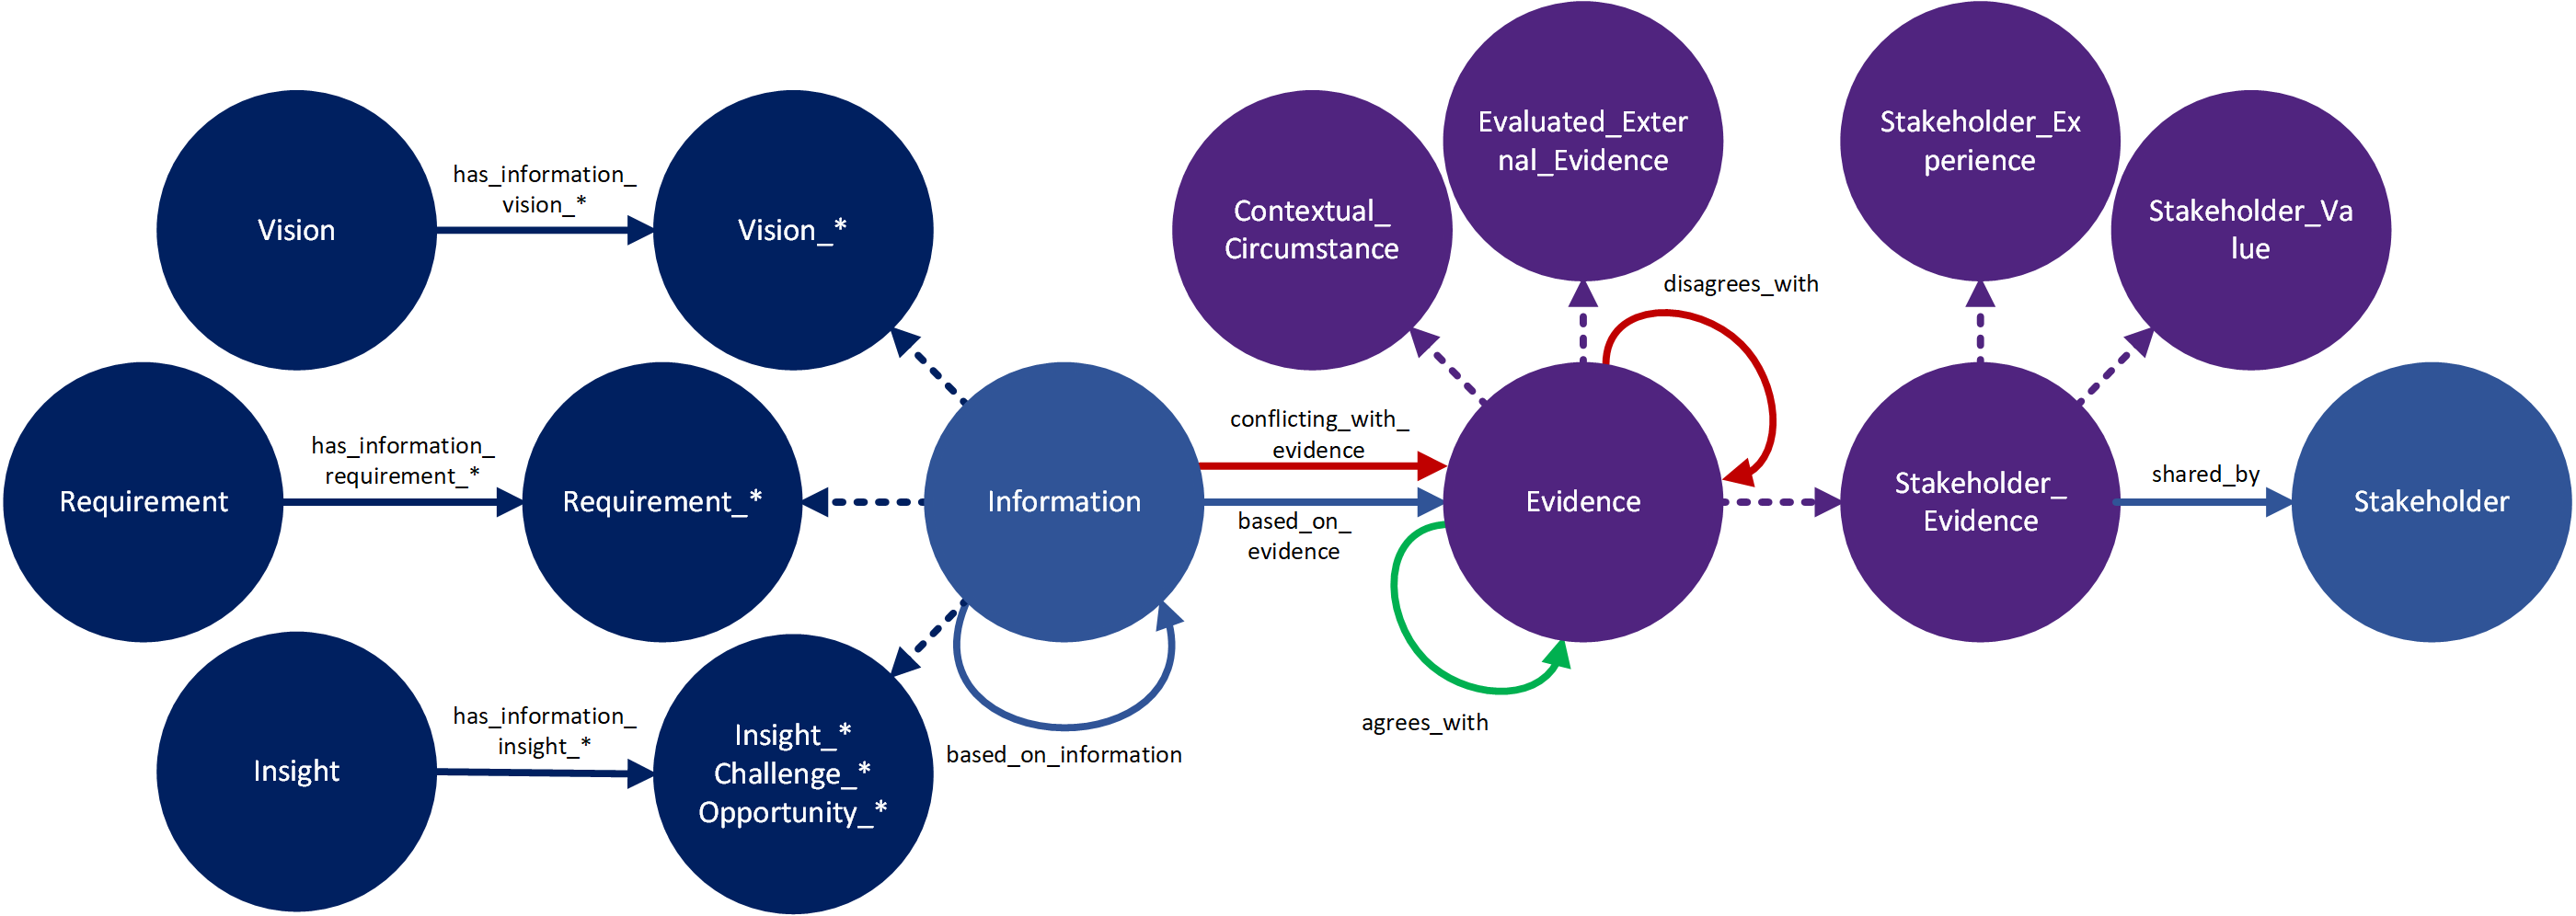
\includegraphics[width=17cm]{../../Images/05_Validation/05_RP_Instantiated.png}
  \caption{The combined requirements prioritisation ontology and the decision design pattern ontology.}
  \label{fig:05_RP_Instantiated}
\end{figure}

\subsubsection{Structural validation}
An incorrect maximum number of violations can cause an incorrect information maturity-level. The structural violations are not part of the functions that define the information maturity-level. Two scenarios can cause an incorrect maximum number of violations:
\begin{enumerate}
\item A requirement does not address an insight. In this case, we cannot retrieve the maximum number of violations for the insight.
\item An insight does not contribute to a vision. In this case, we cannot retrieve the maximum number of violations for the vision.
\end{enumerate}

While the reasoner finds structural violations, the dashboards are not reliable and will not show up. The decision-maker needs to solve the structural violations first.

\paragraph{Structural validation: $Insight$ contributes to $Vision$}
We add the object properties $has\_insight$, $contributes\_to\_vision$, and $in{\f}ormation\_of$ (including the sub-object properties $in{\f}ormation\_of\_requirement$, $in{\f}ormation\_of\_vision$, and $in{\f}ormation\_of\_insight$) to detect the visions that have an $Insight$. The $in{\f}ormation\_of$ object property (and its sub-object properties) are the inverse of the $has\_in{\f}ormation$ object property (and its sub-object properties). The reasoner infers the $contributes\_to\_vision$ object property from the super property figure \ref{fig:05_RP_contributes_to_vision_SP} presents. $has\_insight$ is the inverse of $contributes\_to\_vision$. 

\begin{figure}[H]
\centering
  
\includegraphics[width=17cm]{../../Images/05_Validation/05_RP_Contributes_To_Vision_SP.png}
  \caption{The Prot\'eg\'e configuration of the super property that the reasoner uses to infer the $contributes\_to\_vision$ object property.}
  \label{fig:05_RP_contributes_to_vision_SP}
\end{figure}

Figure \ref{fig:05_RP_contributes_to_vision} presents the super property that infers the $contributes\_to\_vision$ and $has\_insight$ object properties automatically if we can trace an $Insight$ to a $Vision$ using the chain of object properties.

\begin{figure}[H]
\centering
  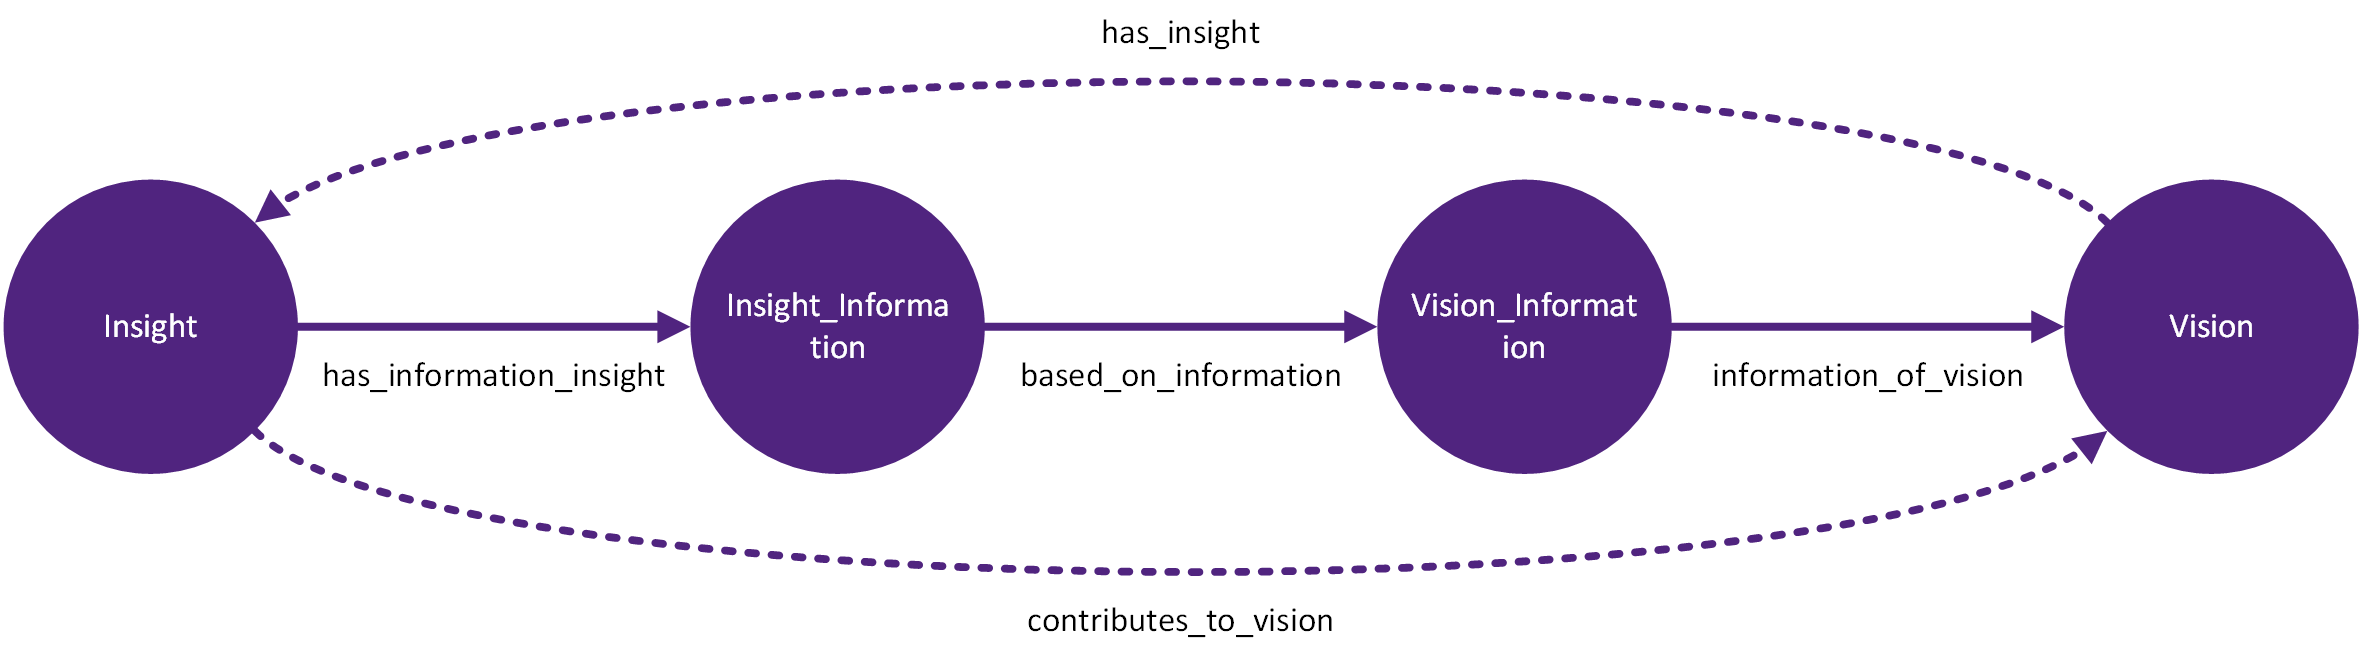
\includegraphics[width=17cm]{../../Images/05_Validation/05_RP_Contributes_To_Vision.png}
  \caption{The super property infers the $contributes\_to\_vision$ and $has\_insight$ object properties automatically if there is a trace from an $Insight$ to a $Vision$ using the chain of object properties. The reasoner infers the dotted lines using the super property.}
  \label{fig:05_RP_contributes_to_vision}
\end{figure}

Code sample \ref{SHACL_RP_STRUC_INSVIS} presents the SHACL shapes we use to detect that an $Insight$ does not contribute to a $Vision$. Without the super property figure \ref{fig:05_RP_contributes_to_vision} presents the constraints would need to validate three object properties on three target classes. In this case, the super property enables the reasoner to infer these three object properties into a single object property. This example shows that inferencing reduces the complexity of the constraints. 

\begin{lstlisting}[float,language=SHACL,caption={The SHACL shapes we use to detect that an $Addressed\_Insight$ does not contribute to a $Vision$.},label={SHACL_RP_STRUC_INSVIS}][H]
rp:Addressed_InsightShape a sh:NodeShape;
	sh:targetClass rp:Addressed_Insight; 
	sh:property [
		sh:path rp:contributes_to_vision;
		sh:severity sh:Violation;
		sh:minCount 1;
		sh:message "Structural: Insight does not contribute to a Vision." ; ];
\end{lstlisting}

\paragraph{Structural validation: $Requirement$ addresses $Insight$}
We want the software product manager to focus on the relevant individuals. Therefore, the constraints should only generate violations for individuals that are relevant for a decision. For example, we need to prevent that an $Insight$ that is not addressed by a $Requirement$ generates a violation. This $Insight$ is not relevant yet. However, the constraints should generate a violation as soon as a $Requirement$ addresses this $Insight$.

First, we use the $Addressed\_Insight$ sub-class to identify the insights that a requirement addresses. Insights that a requirement does not address are not relevant for requirements prioritisation. We use the same concept for the $Addressed\_Opportunity$ and the $ Addressed\_Challenge$. The $Addressed\_Opportunity$ and the $Addressed\_Challenge$ are subclasses of the $Addressed\_Insight$ as well. 

We also want to make sure every requirement that a software product manager prioritises addresses an insight. The reasoner infers the $addresses$ object property from the super property figure \ref{fig:05_RP_Addresses} presents.

\begin{figure}[H]
\centering
  
\includegraphics[width=17cm]{../../Images/05_Validation/05_RP_Addresses.png}
  \caption{The Prot\'eg\'e configuration of the super property that the reasoner uses to infer the $contributes\_to\_vision$ object property.}
  \label{fig:05_RP_Addresses}
\end{figure}

Figure \ref{fig:addressed_requirement} presents the super property that infers the $addresses$ object property automatically if we can trace a $Requirement$ to an $Insight$ using the chain of object properties.

\begin{figure}[H]
\centering
  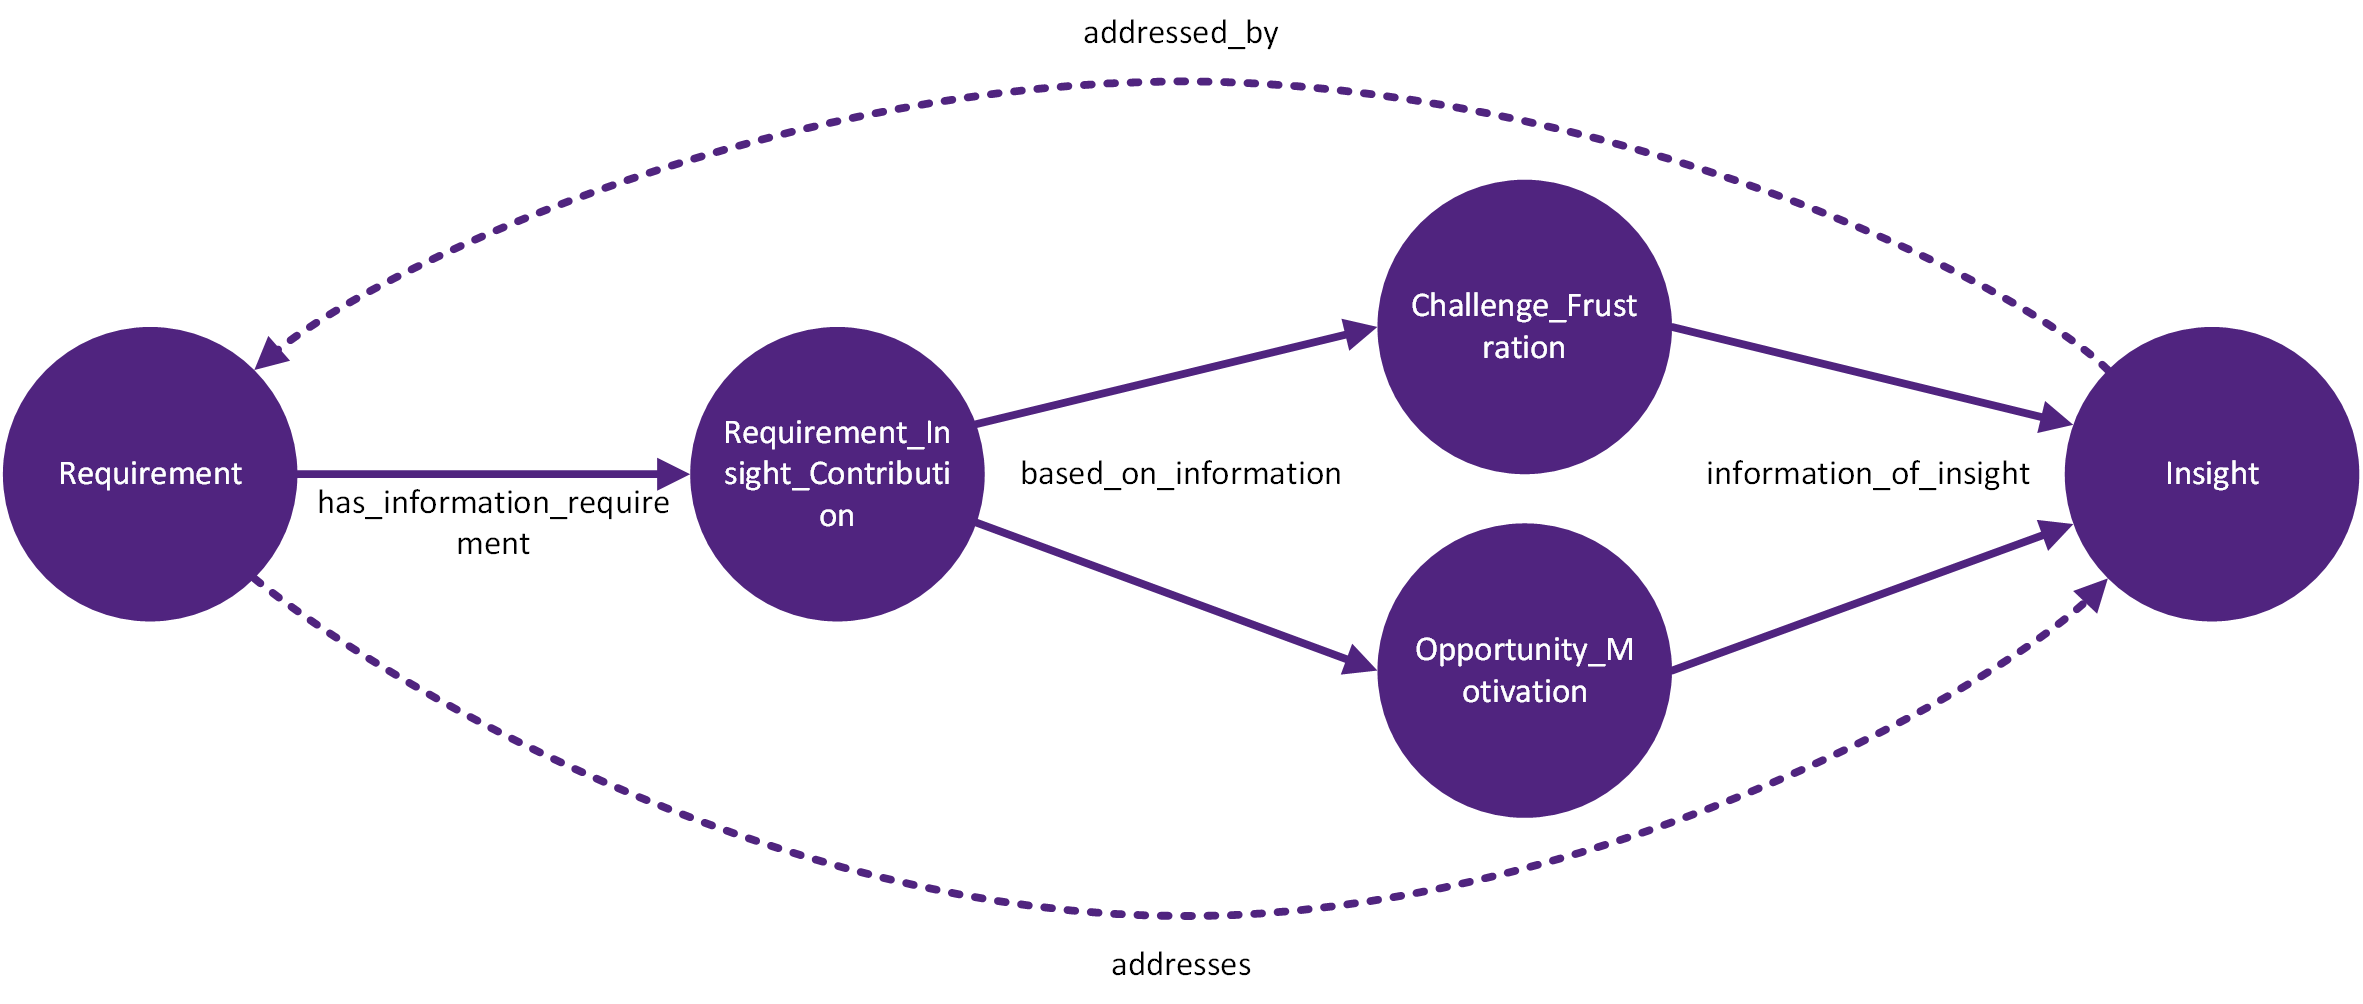
\includegraphics[width=15cm]{../../Images/05_Validation/05_RP_Addresses_Overview.png}
  \caption{The super property that infers the $addresses$ object property automatically if we can trace a $Requirement$ to an $Insight$ using the chain of object properties.}
  \label{fig:addressed_requirement}
\end{figure}

Code sample \ref{SHACL_RP_STRUC_ADD} presents the SHACL shapes we use to detect that a $Requirement$ does not address an $Insight$.

\begin{lstlisting}[float,language=SHACL,caption={The SHACL shapes we use to detect that a $Requirement$ does not address an $Insight$.},label={SHACL_RP_STRUC_ADD}][H]
rp:RequirementShape a sh:NodeShape;
	sh:targetClass rp:Requirement; 
	sh:property [
		sh:path rp:addresses; 
		sh:severity sh:Violation; 
		sh:minCount 1; 
		sh:message "Structural: Requirement does not address an Insight."; 
\end{lstlisting}

\subsubsection{Test scenarios for the decision ontology pattern}
We define six abstract test scenarios. The abstraction makes it easier to validate that a specific scenario triggers the expected violations. Scenario $SC0$ validates the structure of the ontology. The first scenario ($SC1$) should not generate any violations. The other scenarios validate a specific pattern and are structurally valid. This structure limits the complexity of the scenarios and their outcomes. 

\paragraph{Scenario 0 ($SC0$): Structural validation}
The requirements, insights, and visions we use in the other scenarios are structurally valid. Each $Requirement$ addresses at least one $Insight$, and each $Insight$ contributes to at least one $Vision$. We create $Requirement\_SC0$ for this. $Requirement\_SC00$ does not address an $Insight$ and should generate one structural violation and one reproducibility violation. $Requirement\_SC00\_Insight\_Contribution$ generates the reproducibility violation as we did not base it on the motivation of frustration of an insight. This missing link breaks the chain figure \ref{fig:addressed_requirement} presents and generates the structural violation. Figure \ref{fig:RP_SC0_Requirement_SC00_Insight_Contribution} presents the configuration of $Requirement\_SC00\_Insight\_Contribution$ in Prot\'eg\'e.

\begin{figure}[H]
\centering
  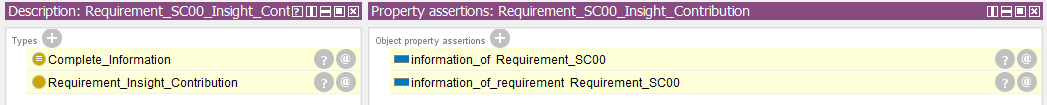
\includegraphics[width=17cm]{../../Images/05_Validation/05_RP_Requirement_SC00_Insight_Contribution.png}
  \caption{The individual $Requirement\_SC00\_Insight\_Contribution$ in Prot\'eg\'e. The $in{\f}ormation\_o{\f}$ object property is the inverse of the $has\_in{\f}ormation$ object property. The reasoner uses this characteristic to infer the $in{\f}ormation\_o{\f}$ object property. }
  \label{fig:RP_SC0_Requirement_SC00_Insight_Contribution}
\end{figure}

Additionally, we define $Requirement\_SC01$. $Requirement\_SC01$ addresses $Opportunity\_SC01$. Therefore $Requirement\_SC01$ should not trigger a structural violation. However, $Opportunity\_SC01$ does not contribute to a $Vision$. $Opportunity\_SC01$ should generate one structural validation and one reproducibility violation. $Opportunity\_SC01\_Vision\_Contribution$ generates the reproducibility violations as we did not base it on vision relevant information. This missing link breaks the chain figure \ref{fig:05_RP_contributes_to_vision} presents and generates the structural violation. Figure \ref{fig:RP_SC0_Opportunity_SC01_Vision_Contribution} presents the configuration of $Opportunity\_SC01\_Vision\_Contribution$ in Prot\'eg\'e.

\begin{figure}[H]
\centering
  \includegraphics[width=17cm]{../../Images/05_Validation/05_RP_Opportunity_SC01_Vision_Contribution}
  \caption{The individual $Opportunity\_SC01\_Vision\_Contribution$ in Prot\'eg\'e. The $in{\f}ormation\_o{\f}$ object property is the inverse of the $has\_in{\f}ormation$ object property. The reasoner uses this characteristic to infer the $in{\f}ormation\_o{\f}$ object property. }
  \label{fig:RP_SC0_Opportunity_SC01_Vision_Contribution}
\end{figure}

We expect $4$ structural violations in scenario $SC0$.

\paragraph{Scenario 1 ($SC1$): Decision ontology pattern}
The information in the first scenario is complete, reproducible, meets the minimum level of consensus, and does not exceed the maximum level of conflict. Figure \ref{fig:RP_SC1_Vision} presents $Vision\_SC1$ as an example. $Vision\_SC1$ is complete based on the $has\_in{\f}ormation\_vision\_current\_state$, $*\_vision\_statement$, $*\_vision\_target\_condition$, and $*\_vision\_measurable\_objective$ object properties.

\begin{figure}[H]
\centering
  \includegraphics[width=17cm]{../../Images/05_Validation/05_RP_SC1_Vision_SC1.png}
  \caption{The individual $Vision\_SC1$ in Prot\'eg\'e. The reasoner infers the $based\_on\_evidence$ object property based on the $agrees\_with$ object property between $Stakeholder\_Value\_SC1$ and $Stakeholder\_Experience\_SC1$.}
  \label{fig:RP_SC1_Vision}
\end{figure}

The completeness pattern requires that each individual classified as $In{\f}ormation$ hosts the $data\_value$ and $data\_description$ data properties. Additionally, the vision statement should also include the $time\_{\f}rame$ data property. The reproducibility pattern requires that individuals classified as $In{\f}ormation$ are $based\_on\_evidence$ or $based\_on\_in{\f}ormation$. The conflict pattern requires that $In{\f}ormation$ individuals do not have conflicting evidence (represented by the object property $conflict\_with\_evidence$). Figure \ref{fig:RP_Vision_SC1_Statement} presents $Vision\_SC1\_Statement$ as an example of a complete and reproducible vision statement. $Vision\_SC1\_Statement$ meets the minimum consensus-level and does not have conflicting evidence.

\begin{figure}[H]
\centering
  \includegraphics[width=17cm]{../../Images/05_Validation/05_RP_SC1_Vision_SC1_Statement.png}
  \caption{The individual $Vision\_SC1\_Statement$ in Prot\'eg\'e. The reasoner infers the $based\_on\_evidence$ object properties using the $agrees\_with$ object property between $Stakeholder\_Value\_SC1$ and $Stakeholder\_Experience\_SC1$.}
  \label{fig:RP_Vision_SC1_Statement}
\end{figure}

The consensus pattern requires that each individual classified as $Evidence$ agrees with at least one other evidence source. Figure \ref{fig:RP_Stakeholder_Value_SC1} presents $Stakeholder\_Value\_SC1$. $Stakeholder\_Value\_SC1$ agrees with $Stakeholder\_Experience\_SC1$. The reasoner infers that $Vision\_SC1\_Statement$ $based\_on\_evidence$ $Stakeholder\_Experience\_SC1$ from this. Figure \ref{fig:RP_Vision_SC1_Statement} presents the inferred object property.

\begin{figure}[H]
\centering
  \includegraphics[width=17cm]{../../Images/05_Validation/05_RP_SC1_Stakeholder_Value_SC1.png}
  \caption{The individual $Stakeholder\_Value\_SC1$ in Prot\'eg\'e. $Stakeholder\_Value\_SC1$ agrees with $Stakeholder\_Experience\_SC1$. The reasoner infers that $Vision\_SC1\_Statement$ $based\_on\_evidence$ $Stakeholder\_Experience\_SC1$ from this.}
  \label{fig:RP_Stakeholder_Value_SC1}
\end{figure}

We expect $0$ violations of the completeness pattern in scenario $SC1$.

\paragraph{Scenario 2 ($SC2$): Completeness pattern}
In the second scenario, we attempt to detect incomplete information. We cannot reproduce missing information, and we cannot define a consensus or conflict-level for unreproducible information. As a result, the reproducibility, consensus, and conflict patterns are not relevant in this scenario.

We validate the completeness in two ways. The root classes need to have the specified object properties to the $In{\f}ormation$ classes, and the $In{\f}ormation$ classes need to have the data properties $data\_value$ and $data\_description$. Figure \ref{fig:RP_SC2_Completeness} presents a limited example of the root class $Challenge\_SC2$ and three of the related $In{\f}ormation$ classes. The $Challenge\_SC2\_Reach$ and $Challenge\_SC2\_Business\_Case$ are complete. However, the $Insight$ itself misses the $Insight\_Vision\_Contribution$ and $Challenge\_Frustration$. 

Additionally, $Challenge\_SC2\_Value$ misses the $data\_value$ and $data\_description$ data properties. We expect six violations related to $Challenge\_SC2$. Those six violations cover the missing $Challenge\_Frustration$, $Insight\_Vision\_Contribution$, and their related $data\_value$ and $data\_description$. Additionally, we expect and two violations related to $Challenge\_SC2\_Value$.

\begin{figure}[H]
\centering
  \includegraphics[width=17cm]{../../Images/05_Validation/05_RP_SC2_Completeness.png}
  \caption{An incomplete example of the root class $Insight$ and three of the related $In{\f}ormation$ classes.}
  \label{fig:RP_SC2_Completeness}
\end{figure}

Figure \ref{fig:RP_SC2_Challenge_SC2} presents $Challenge\_SC2$ in Prot\'eg\'e. The reasoner infers the $Addressed\_Challenge$ type from the $addressed\_by$ object property and infers the $has\_in{\f}ormation$ object properties from the specific $has\_in{\f}ormation\_$ object properties. For example, the reasoner infers $has\_information$ $Challenge\_SC2\_Value$ from $has\_in{\f}ormation\_insight\_value$ $Challenge\_SC2\_Value$.

\begin{figure}[H]
\centering
  \includegraphics[width=17cm]{../../Images/05_Validation/05_RP_SC2_Challenge_SC2.png}
  \caption{The individual $Challenge\_SC2$ in Prot\'eg\'e. The reasoner infers the $Addressed\_Challenge$ type from the $addressed\_by$ object property and infers the $has\_in{\f}ormation$ object properties from the specific $has\_in{\f}ormation\_$ object properties.}
  \label{fig:RP_SC2_Challenge_SC2}
\end{figure}

We defined $Opportunity\_SC2$, $Requirement\_SC2$, and $Vision\_SC2$ as partially incomplete individuals. 

$Opportunity\_SC2$ refers to $2$ out of the $5$ individuals that store information. The $3$ missing individuals should generate $3$ violations each. Out of these $3$ individuals, $1$ is complete considering the $data\_value$ and $data\_description$. We expect $Opportunity\_SC2$ to trigger $(3*3)+(1*2)=11$ violations. 

$Requirement\_SC2$ refers to $4$ out of the $10$ individuals that store information. The $6$ missing individuals should generate $3$ violations each. Out of these $3$ individuals, $2$ are complete considering the $data\_value$ and $data\_description$. We expect $Requirement\_SC2$ to trigger $(6*3)+(2*2)=22$ violations. 

$Vision\_SC2$ refers to $1$ out of the $4$ individuals that store information. The measurable objective is among the missing $3$ individuals. The measurable objective should generate $4$ violations: $1$ for the individual itself, $1$ for the missing $data\_value$, $1$ for the missing $data\_description$, and $1$ for the missing $time\_{\f}rame$. The other missing individuals should generate $3$ violations each. The individuals are complete considering the $data\_value$ and $data\_description$. We expect $Vision\_SC2$ to trigger $4+(2*3)+(0*2)=10$ violations. 

We expect $43$ violations of the completeness pattern in scenario $SC2$.

\paragraph{Scenario 3 ($SC3$): Reproducibility}
Scenario $SC3$ contains information that is complete and unreproducible. We cannot define the consensus and conflict-level when information is not reproducible. As a result, the consensus and conflict patterns are not relevant in this scenario. 

We create $23$ individuals that are not reproducible. These individuals are not evidence-based and are not related to $In{\f}ormation$ using the $based\_on\_information$ object property. For example, $Requirement\_SC3\_Value$ contains the $data\_value$ and $data\_description$ data properties. Therefore, $Requirement\_SC3\_Value$ is complete. However, $Requirement\_SC3\_Value$ is not related to evidence or information. We expect $1$ violation related to $Requirement\_SC3\_Value$. Figure \ref{fig:RP_SC4_Requirement_SC3_Value} presents $Requirement\_SC3\_Value$ in Prot\'eg\'e.

\begin{figure}[H]
\centering
  \includegraphics[width=17cm]{../../Images/05_Validation/05_RP_SC3_Requirement_SC3_Value.png}
  \caption{The individual $Requirement\_SC3\_Value$ in Prot\'eg\'e. The $in{\f}ormation\_o{\f}$ object property is the inverse of the $based\_on\_information$ object property. $Requirement\_SC3$ is based on $Requirement\_SC3\_Value$. The reasoner infers the $in{\f}ormation\_o{\f}$ from its inverse.}
  \label{fig:RP_SC4_Requirement_SC3_Value}
\end{figure}

We define $4$ root individuals for which we validate the reproducibility: $Opportunity\_SC3$, $Challenge\_SC3$, $Requirement\_SC3$, and $Vision\_SC3$. $Opportunity\_SC3$ requires $3$ knowledge criteria, $Challenge\_SC3$ requires $3$ knowledge criteria as well, and $Requirement\_SC3$ requires $4$ knowledge criteria. We base these $10$ knowledge criteria on another $13$ information sources spread out over $Opportunity\_SC3$, $Challenge\_SC3$, $Requirement\_SC3$, and $Vision\_SC3$. As a result, we expect $23$ violations of the reproducibility pattern in scenario $SC3$.

\paragraph{Scenario 4 ($SC4$): Conflict pattern}
In scenario $SC4$, we validate that the information is complete, reproducible, and does not cause any conflict. Figure \ref{fig:RP_SC4_Conflict} presents how this evidence disagrees with each other. Figure \ref{fig:RP_SC4_Stakeholder_Experience_SC4} presents $Stakeholder\_Experience\_SC4$ in Prot\'eg\'e.

\begin{figure}[H]
\centering
  \includegraphics[width=15cm]{../../Images/05_Validation/05_SC4_Conflict_Inference.png}
  \caption{$4$ evidence sources disagree with each other. The fixed lines represent configured object properties. The dotted lines represent inferred object properties.}
  \label{fig:RP_SC4_Conflict}
\end{figure}

\begin{figure}[H]
\centering
  \includegraphics[width=17cm]{../../Images/05_Validation/05_RP_SC4_Stakeholder_Experience_SC4.png}
  \caption{The individual $Stakeholder\_Experience\_SC4$ in Prot\'eg\'e. The reasoner infers the $disagrees\_with$ object property using its symmetric and irreflexive characteristics.}
  \label{fig:RP_SC4_Stakeholder_Experience_SC4}
\end{figure}

For example, we use $Contextual\_Circumstance\_SC4$ as evidence for $Challenge\_SC4\_Business\_Case$. $Contextual\_Circumstance\_SC4$ disagrees with $Evaluated\_External\_Evidence\_SC4$. As a result, $Challenge\_SC4\_Business\_Case$ conflicts with these evidence sources. We expect $2$ violations related to $Challenge\_SC4\_Business\_Case$: $1$ for each evidence conflict. Figure \ref{fig:RP_SC4_Protege_Challenge_SC4_Business_Case} presents $Challenge\_SC4\_Business\_Case$ in Prot\'eg\'e.

\begin{figure}[H]
\centering
  \includegraphics[width=17cm]{../../Images/05_Validation/05_RP_SC4_Challenge_SC4_Business_Case.png}
  \caption{The individual $Challenge\_SC4\_Business_Case$ in Prot\'eg\'e. The reasoner infers the $conflict\_with\_evidence$ object property from the super property figure \ref{fig:conflict_transitive} in section \ref{odp_conflict} \nameref{odp_conflict} presents.}
  \label{fig:RP_SC4_Protege_Challenge_SC4_Business_Case}
\end{figure}

We define $4$ conflicting evidence sources: $Contextual\_Circumstance\_SC4$, $Evaluated\_External\_Evidence\_SC4$ and $Stakeholder\_Value\_SC4$, $Stakeholder\_Experience\_SC4$\footnote{$Stakeholder\_Experience\_SC4$ and $Stakeholder\_Value\_SC4$ are shared by $Stakeholder\_SC4$ to ensure this evidence does not trigger any reproducibility violations.}. We based $16$ individuals on these evidence sources: $3$ individuals that host information for $Challenge\_SC4$, $3$ individuals that host information for $Opportunity\_SC4$, $6$ individuals that host information for, $Requirement\_SC4$, and another $4$ individuals that host information for $Vision\_SC4$. As a result, we expect $16$ violations of the conflict pattern in scenario $SC4$.

\paragraph{Scenario 5 ($SC5$): Consensus pattern}
The last scenario contains information that is complete and reproducible. It does not contain evidence conflicts. However, some information does not meet the defined consensus constraints. Each individual that the reasoner classifies as $Used\_Evidence$ should have at least one $agrees\_with$ object property to meet the consensus constraints. 

We have created $4$ evidence sources for scenario $SC5$: $Contextual\_Circumstance\_SC5$, $Evaluated\_External\_Evidence\_SC5$, $Stakeholder\_Experience\_SC5$, and $Stakeholder\_Value\_SC5$. These evidence sources serve as evidence for the $In{\f}ormation$ related to $SC5$, for example, $Opportunity\_SC5\_Reach$. $Stakeholder\_Experience\_SC5$ and $Stakeholder\_Value\_SC5$ agree with each other and should, therefore, not trigger any violations. Figure \ref{fig:05_RP_SC5_Stakeholder_Value_SC5} presents $Stakeholder\_Value\_SC5$ in Prot\'eg\'e.

\begin{figure}[H]
\centering
  \includegraphics[width=17cm]{../../Images/05_Validation/05_RP_SC5_Stakeholder_Value_SC5.png}
  \caption{The $Stakeholder\_Value\_SC5$ in Prot\'eg\'e. The reasoner infers the $agrees\_with$ object property based its symmetric characteristic.}
  \label{fig:05_RP_SC5_Stakeholder_Value_SC5}
\end{figure}

Figure \ref{fig:05_RP_SC5_Evaluated_External_Evidence_SC5} presents, for example, $Evaluated\_External\_Evidence\_SC5$ in Prot\'eg\'e. $Evaluated\_External\_Evidence\_SC5$ is used as evidence for $Requirement\_SC5\_Increase\_Revenue$ and is, therefore, classified as $Used\_Evidence$. However, it does not have an $agrees\_with$ object property and should generate $1$ violation. $Contextual\_Circumstance\_SC5$ does not have an $agrees\_with$ and should generate $1$ violation as well.

\begin{figure}[H]
\centering
  \includegraphics[width=17cm]{../../Images/05_Validation/05_RP_SC5_Evaluated_External_Evidence_SC5.png}
  \caption{The $Evaluated\_External\_Evidence\_SC5$ in Prot\'eg\'e. The $evidence\_used\_{\f}or$ object property is the inverse of the $based\_on\_evidence$ object property. The reasoner uses this inverse characteristic to infer the $evidence\_used\_{\f}or$ object property.}
  \label{fig:05_RP_SC5_Evaluated_External_Evidence_SC5}
\end{figure}

As a result, we expected $2$ violations of the consensus pattern in scenario $SC5$.

\paragraph{The result of the test scenarios}
Table \ref{table:rp_number_of_violations} presents the results of the tests. We detect $88$ violations. Figure \ref{fig:RP_SC_Results} presents an extract of the results as the SHACL4P plugin presents them in Prot\'eg\'e.

\begin{table}[H]
\centering
\caption{The number of expected and detected violations per scenario and pattern.}
\begin{tabular}{| p{3cm} | p{3cm} | p{4cm} | p{4cm} | }
\hline
\rowcolor{document}
\color{documentText}Scenario & \color{documentText}Scenario & \color{documentText}Expected violations & \color{documentText}Detected violations  \\
\hline
$SC0$ & Structural & 4 & 4 \\
\hdashline
$SC1$ & n/a & 0 & 0 \\
\hdashline
$SC2$ & Completeness & 43 & 43 \\
\hdashline
$SC3$ & Reproducibility & 23 & 23 \\
\hdashline
$SC4$ & Conflict & 16 & 16 \\
\hdashline
$SC5$ & Consensus & 2 & 2 \\
\hline
\end{tabular}
\label{table:rp_number_of_violations}
\end{table}

\begin{figure}[H]
\centering
  \includegraphics[width=17cm]{../../Images/05_Validation/05_RP_SC_Results.png}
  \caption{An extract of the results as the SHACL4P plugin presents them in Prot\'eg\'e.}
  \label{fig:RP_SC_Results}
\end{figure}

\subsubsection{Decision-relevant root individuals}
We determine the decision root individual that are relevant for a specific requirements prioritisation decision. The requirement prioritisation decision requires two individuals that are both classified as $Requirement$: $r_1$ and $r_2$. We know that a requirement needs to address an insight and that an insight has two sub-classes: opportunity and challenge. We also know that a vision should reproduce an insight. Code sample \ref{SPARQL_RP_VAL_Related} presents a SPARQL query that retrieves all opportunities, challenges, and visions related to a requirement using parameters $<r1>$ and $<r2>$. We execute the SPARQL query and feed the results into the set $RI$. We define function $rpri(r_1,r_2) = RI$ to logically represent the SPARQL query. We manually add $r_1$ and $r_2$ to $RI$.

\begin{lstlisting}[float,language=SPARQL1,caption={The first part of the SPARQL query gathers the insight(s) related to the specified requirements based on the $addresses$ object property: a $Requirement$ $addresses$ an insight. The second part of the SPARQL query gathers the vision(s) related to the specified requirements based on the $addresses$, $has\_in{\f}ormation$, and $based\_on\_in{\f}ormation$ object properties.},label={SPARQL_RP_VAL_Related}][H]
SELECT DISTINCT ?ri 
WHERE 
{
	# Gather insights (opportunities and challenges)
	{
		?req rp:addresses ?ri .
		?ri rdf:type ?t
		FILTER(?t != owl:Thing && ?t != rp:Addressed_Insight &&	?t != rp:Addressed_Opportunity && ?t != rp:Addressed_Challenge && ?t != rp:Insight).
	}
	UNION
	# Gather visions
	{
		?req rp:addresses ?ins .
		?ins rp:has_information ?ivc .
		?ivc rdf:type rp:Insight_Vision_Contribution .
		?ivc rp:based_on_information ?vcs .
		?ri rp:has_information ?vcs .
		?ri rdf:type ?t .	
		FILTER(?t != owl:Thing).				
	}
	FILTER(?req = <r1> || ?req = <r2>)
}
\end{lstlisting}

\subsubsection{Test scenarios for the decision presentation pattern}
We use four requirements to validate the decision presentation pattern. Each requirement has a different information maturity-level. The software product manager prioritises $Requirement\_SC1$ and $Requirement\_SC2$ in test scenario $DEC1$. The software product manager prioritises $Requirement\_SC3$ and $Requirement\_SC4$ in test scenario $DEC2$.

% ========================================================== DEC1 ===============================================================================================

\paragraph{Decision $DEC1$: $Requirement\_SC1$ versus $Requirement\_SC2$}
A software product manager needs to decide if $Requirement\_SC1$ is more important than $Requirement\_SC2$. The first question we ask is:

\begin{center}
\large\color{document}{Is the information ready for an evidence-based decision?}
\end{center}

The first dashboard of the decision presentation pattern helps the decision-maker to answer this question. We define the consolidated information maturity-level, and the evidence spread for these two requirements to generate this dashboard. 

We use function $rpri(Requirement\_SC1,Requirement\_SC2)$ to define $RI_{DEC1}$. $RI_{DEC1}$ is the set of decision-relevant root individuals. $RI_{DEC1}$ includes $Challenge\_SC1$, $Opportunity\_SC1$, $Challenge\_SC2$, $Opportunity\_SC2$, $Vision\_SC1$, and $Vision\_SC2$. We manually add $Requirement\_SC1$ and $Requirement\_SC2$ to $RI_{DEC1}$. Table \ref{table:rp_maximum_evidence_sc1} presents the maximum and the actual number of violations per decision-relevant root individual. We conclude that decision $DEC1$ can generate up to $239$ violations, and that decision $DEC1$ generates $52$ violations.

\begin{table}[H]
\centering
\caption{The maximum and the actual number of violations per decision-relevant root individual.}
\begin{tabular}{| p{3cm} | p{0.8cm} | p{0.8cm} | p{0.8cm} | p{0.8cm} | p{1.2cm} | p{0.8cm} | p{0.8cm} | p{0.8cm} | p{0.8cm} | p{1.2cm} |}
\hline
\rowcolor{document}
\color{documentText}Function & \color{documentText}$mvi_1$ & \color{documentText}$mvi_2$ & \color{documentText}$mvi_3$ & \color{documentText}$mvi_4$ & \color{documentText}$Total_{mv}$ & \color{documentText}$avi_1$ & \color{documentText}$avi_2$ & \color{documentText}$avi_3$ & \color{documentText}$avi_4$ & \color{documentText}$Total_{av}$ \\
\hline
$Requirement\_SC1$ 	& 30 & 10 & 2 & 10 & 52 & 0 & 0 & 0 & 0 & 0\\
\hdashline
$Challenge\_SC1$ 	& 15 & 5 & 2 & 5 & 27 & 0 & 0 & 0 & 0 & 0\\
\hdashline
$Opportunity\_SC1$ 	& 15 & 5 & 2 & 5 & 27 & 0 & 0 & 0 & 0 & 0\\
\hdashline
$Vision\_SC1$ 		& 14 & 4 & 2 & 4 & 24 & 0 & 0 & 0 & 0 & 0\\ 
\hdashline
$Requirement\_SC2$ 	& 30 & 10 & 4 & 10 & 54 & 23 & 0 & 0 & 0 & 22 \\ 
\hdashline
$Opportunity\_SC2$ 	& 15 & 5 & 4 & 5 & 29 & 11 & 0 & 0 & 0 & 11 \\ 
\hdashline
$Vision\_SC2$ 		& 14 & 4 & 4 & 4 & 26 & 10 & 0 & 0 & 0 & 10 \\
\hdashline
Total 				& 133 & 43 & 20 & 43 & 239 & 44 & 0 & 0 & 0 & 44 \\
\hline
\end{tabular}
\label{table:rp_maximum_evidence_sc1}
\end{table}

The information table \ref{table:rp_maximum_evidence_sc1} presents allows us to calculate the information maturity-level $iml$ for decision $DEC1$. Equation \ref{eq:information_maturity_level_SC1} shows that the information maturity-level for $DEC1$ is 82\%.

\begin{equation} \label{eq:information_maturity_level_SC1}
iml(RI) = \dfrac{mv_(RI)-av(RI)}{mv(RI)} = \dfrac{239-44}{239} = 0.816
\end{equation}

The first dashboard also presents the evidence spread. Table \ref{table:rp_evidence_spread_SC1} presents the evidence spread for decision $DEC1$ using the SPARQL query code sample \ref{SPARQL_ES} presents.

\begin{table}[H]
\centering
\caption{The evidence spread for the decision-relevant root individuals and the total evidence spread for this scenario.}
\begin{tabular}{| p{5cm} | p{4cm} |  p{4cm} |  p{2cm} | }
\hline
\rowcolor{document}
\color{documentText}Evidence &\color{documentText}$Requirement\_SC1$ & \color{documentText}$Requirement\_SC2$ & \color{documentText}Total \\
\hline
$Contextual\_Circumstance$ & 9 & 3 & 12 \\
\hdashline
$Stakeholder\_Value$ & 7 & 3 & 10 \\
\hdashline
$Evaluated\_External\_Evidence$ & 9 & 3 & 12 \\
\hdashline
$Stakeholder\_Experience$ & 7 & 3 & 10 \\
\hline
\end{tabular}
\label{table:rp_evidence_spread_SC1}
\end{table}

Figure \ref{fig:05_RP_Dashboard_Component_1_RP_SC1} presents a mock-up of the first decision presentation pattern dashboard. The dashboard reflects an information maturity-level of 82\% and the evidence spread table \ref{table:rp_evidence_spread_SC1} presents. The decision-maker needs to decide if the information maturity-level and evidence-spread are acceptable, depending on the impact of the decision.

\begin{figure}[H]
\centering
  \includegraphics[width=14cm]{../../Images/05_Validation/05_RP_Dashboard_Component_1_RP_SC1.png}
  \caption{A mock-up of the first decision presentation pattern dashboard for decision $DEC1$. The dashboard reflects an information maturity-level of 82\% and the evidence spread table \ref{table:rp_evidence_spread_SC1} presents.}
  \label{fig:05_RP_Dashboard_Component_1_RP_SC1}
\end{figure}

The second dashboard of the decision presentation pattern presents the information maturity-level per pattern. We present the pattern-specific maximum and the actual violations in table \ref{table:rp_maximum_evidence_sc1}.

$Requirement\_SC1$ does not generate any completeness violations. $Requirement\_SC2$ generates $44$ completeness violations. The completeness pattern can generate up to $133$ violations in total for decision $DEC1$. $Requirement\_SC1$ and $Requirement\_SC2$ do not generate any other violations. 

Figure \ref{fig:05_RP_Dashboard_Component_2_RP_SC1} presents a mock-up of the second decision presentation pattern dashboard. The dashboard reflects the completeness maturity-level of $\dfrac{133-44}{133} = 0.669$, which results in 67\%. The maturity-levels of the other patterns are 100\% as they do not generate any violations.

\begin{figure}[H]
\centering
  \includegraphics[width=17cm]{../../Images/05_Validation/05_RP_Dashboard_Component_2_RP_SC1.png}
  \caption{A mock-up of the second decision presentation pattern dashboard for decision $DEC1$. The dashboard reflects a completeness maturity-level of 67\%.}
  \label{fig:05_RP_Dashboard_Component_2_RP_SC1}
\end{figure}

To complete the missing information, the software product manager needs to know which information is incomplete. The third dashboard of the decision presentation pattern presents the completeness of information per decision-relevant individual.

Figure \ref{fig:05_RP_Dashboard_Component_3_RP_SC1_Completeness} presents a mock-up of the third decision presentation pattern dashboard, considering the software product manager selects $Opportunity\_SC2$. We observe that three decision-relevant individuals are incomplete. The bar charts give the software product manager an indication which individuals are causing the 67\% completeness maturity-level. The software product manager wants to know more information on a specific individual: $Opportunity\_SC2$. The dashboard presents the violations related to $Opportunity\_SC2$ in the table below the bar chart. We also observe the consolidation into root individuals: individuals classified as $Vision$, $Requirement$, $Opportunity$, or $Challenge$ are root individuals. The dashboard consolidates the violations of $Opportunity\_SC2\_Value$ under $Opportunity\_SC2$.

\begin{figure}[H]
\centering
  \includegraphics[width=16cm]{../../Images/05_Validation/05_RP_Dashboard_Component_3_RP_SC1_Completeness.png}
  \caption{A mock-up of the third decision presentation pattern dashboard, considering the decision-maker selected $Opportunity\_SC2$. We observe that four decision-relevant individuals are incomplete.}
  \label{fig:05_RP_Dashboard_Component_3_RP_SC1_Completeness}
\end{figure}

The software product manager wants to understand the reproducibility of the information. Figure \ref{fig:05_RP_Dashboard_Component_3_RP_SC1_Spread} presents the evidence spread using the third dashboard, considering the decision-maker clicked on the pie chart presenting the evidence spread in the first dashboard. This evidence spread does not violate any constraints. However, the software product manager can improve the evidence spread by elaborating on, for example, $Vision\_SC1$, which is based on two out of four evidence types.

\begin{figure}[H]
\centering
  \includegraphics[width=16cm]{../../Images/05_Validation/05_RP_Dashboard_Component_3_RP_SC1_Spread.png}
  \caption{The evidence spread using the third dashboard, considering the decision-maker selected $Challenge\_SC1$. We observe that, for example, $Stakeholder\_Value$ and $Stakeholder\_Experience$ reproduce $Vision\_SC1$.}
  \label{fig:05_RP_Dashboard_Component_3_RP_SC1_Spread}
\end{figure}

% ========================================================== DEC2 ===============================================================================================

\paragraph{Decision $DEC2$: $Requirement\_SC3$ versus $Requirement\_SC4$}
A software product manager needs to decide if $Requirement\_SC3$ is more important than $Requirement\_SC4$. The first question we ask is:

\begin{center}
\large\color{document}{Is the information ready for this decision?}
\end{center}

The first decision presentation pattern dashboard helps a decision-maker to answer this question. We define the consolidated information maturity-level, and the evidence spread for the two requirements to generate this dashboard. 

We use function $rpri(Requirement\_SC3,Requirement\_SC4)$ to define $RI_{DEC2}$. $RI_{DEC2}$ is the set of decision-relevant root individuals. $RI_{DEC2}$ includes $Challenge\_SC3$, $Opportunity\_SC3$, $Challenge\_SC4$, $Opportunity\_SC4$, $Vision\_SC3$, and $Vision\_SC4$. We manually add $Requirement\_SC3$ and $Requirement\_SC4$ to $RI_{DEC2}$. Table \ref{table:rp_maximum_evidence_sc2} presents the maximum and the actual number of violations per decision-relevant root individual. The bottom line of the table presents the maximum and the actual number of violations per pattern. We conclude that decision $DEC2$ can generate up to $252$ violations. We conclude that decision $DEC2$ generates $37$ violations.

\begin{table}[H]
\centering
\caption{The maximum number of violations per decision-relevant root individual.}
\begin{tabular}{| p{3cm} | p{0.8cm} | p{0.8cm} | p{0.8cm} | p{0.8cm} | p{1.2cm} | p{0.8cm} | p{0.8cm} | p{0.8cm} | p{0.8cm} | p{1.2cm} |}
\hline
\rowcolor{document}
\color{documentText}Function & \color{documentText}$mvi_1$ & \color{documentText}$mvi_2$ & \color{documentText}$mvi_3$ & \color{documentText}$mvi_4$ & \color{documentText}$Total_{mv}$ & \color{documentText}$avi_1$ & \color{documentText}$avi_2$ & \color{documentText}$avi_3$ & \color{documentText}$avi_4$ & \color{documentText}$Total_{av}$ \\
\hline
$Requirement\_SC3$ 	& 30 & 10 & 0 & 10 & 50 & 0 & 9 & 0 & 0 & 9\\
\hdashline
$Challenge\_SC3$ 	& 15 & 5 & 0 & 5 & 25 & 0 & 4 & 0 & 0 & 4 \\
\hdashline
$Opportunity\_SC3$ 	& 15 & 5 & 0 & 5 & 25 & 0 & 4 & 0 & 0 & 4 \\
\hdashline
$Requirement\_SC4$ 	& 30 & 10 & 2 & 10 & 52 & 0 & 0 & 0 & 6 & 6 \\
\hdashline
$Challenge\_SC4$ 	& 15 & 5 & 2 & 5 & 27 & 0 & 0 & 0 & 3 & 3 \\ 
\hdashline
$Opportunity\_SC4$ 	& 15 & 5 & 2 & 5 & 27 & 0 & 0 & 0 & 3 & 3 \\ 
\hdashline
$Vision\_SC3$ 		& 14 & 4 & 0 & 4 & 22& 0 & 4 & 0 & 0 & 4 \\
\hdashline
$Vision\_SC4$ 		& 14 & 4 & 2 & 4 & 24 & 0 & 0 & 0 & 4 & 4 \\
\hdashline
Total 				& 148 & 48 & 8 & 48 & 252 & 0 & 21 & 0 & 16 & 37 \\
\hline
\end{tabular}
\label{table:rp_maximum_evidence_sc2}
\end{table}

The information presented in table \ref{table:rp_maximum_evidence_sc2} allows us to calculate the information maturity-level $iml$ for decision $DEC2$. Equation \ref{eq:information_maturity_level_SC2} shows that the information maturity-level for $DEC2$ is 85\%.

\begin{equation} \label{eq:information_maturity_level_SC2}
iml(RI) = \dfrac{mv_(RI)-av(RI)}{mv(RI)} = \dfrac{252-37}{252} = 0.853
\end{equation}

The first dashboard also presents the evidence spread. Table \ref{table:rp_evidence_spread_SC2} presents the evidence spread for decision $DEC2$ using the SPARQL query code sample \ref{SPARQL_ES} presents.

\begin{table}[H]
\centering
\caption{The evidence spread for the decision-relevant root individuals and the total evidence spread for this scenario.}
\begin{tabular}{| p{5cm} | p{4cm} |  p{4cm} |  p{2cm} | }
\hline
\rowcolor{document}
\color{documentText}Evidence &\color{documentText}$Requirement\_SC3$ & \color{documentText}$Requirement\_SC4$ & \color{documentText}Total \\
\hline
$Contextual\_Circumstance$ & 0 & 13 & 13 \\
\hdashline
$Stakeholder\_Value$ & 0 & 13 & 13 \\
\hdashline
$Evaluated\_External\_Evidence$ & 0 & 3 & 3 \\
\hdashline
$Stakeholder\_Experience$ & 0 & 3 & 3 \\
\hline
\end{tabular}
\label{table:rp_evidence_spread_SC2}
\end{table}

Figure \ref{fig:05_RP_Dashboard_Component_1_RP_SC2} presents a mock-up of the decision presentation pattern first dashboard. The dashboard reflects an information maturity-level of 85\% and the evidence spread table \ref{table:rp_evidence_spread_SC2} presents. The decision-maker needs to decide if the information maturity-level and evidence-spread are acceptable, depending on the impact of the decision.

\begin{figure}[H]
\centering
  \includegraphics[width=14cm]{../../Images/05_Validation/05_RP_Dashboard_Component_1_RP_SC2.png}
  \caption{A mock-up of the first decision presentation pattern dashboard for test scenario $DEC2$. The dashboard reflects an information maturity-level of 85\% and the evidence spread table \ref{table:rp_evidence_spread_SC2} presents.}
  \label{fig:05_RP_Dashboard_Component_1_RP_SC2}
\end{figure}

The second decision presentation pattern dashboard presents the information maturity-level per pattern. We present the pattern-specific maximum and the actual violations in table \ref{table:rp_maximum_evidence_sc2}.

$Requirement\_SC3$ and $Requirement\_SC4$ do not generate any completeness violations. We use $Requirement\_SC3$ to test the reproducibility pattern, and it generates $21$ reproducibility violations. The reproducibility pattern can generate up to $48$ violations for decision $DEC2$. We use $Requirement\_SC4$ to test the conflict pattern, and it generates $16$ conflict violations. The conflict pattern can generate up to $48$ violations for decision $DEC2$. $Requirement\_SC3$ and $Requirement\_SC4$ do not generate any other violations. 

Figure \ref{fig:05_RP_Dashboard_Component_2_RP_SC2} presents a mock-up of the second decision presentation pattern dashboard. The dashboard reflects the reproducibility maturity-level of $\dfrac{48-21}{48} = 0.563$, which results in 56\% and the conflict maturity-level of $\dfrac{48-16}{48} = 0.667$, which results in 67\%. The maturity-levels of the other patterns are 100\% as they do not generate any violations.

\begin{figure}[H]
\centering
  \includegraphics[width=17cm]{../../Images/05_Validation/05_RP_Dashboard_Component_2_RP_SC2.png}
  \caption{A mock-up of the second decision presentation pattern dashboard for decision $DEC2$. The dashboard reflects a reproducibility maturity-level of 56\% and a conflict maturity-level of 67\%.}
  \label{fig:05_RP_Dashboard_Component_2_RP_SC2}
\end{figure}

Figure \ref{fig:05_RP_Dashboard_Component_3_RP_SC2_Reproducibility} presents a mock-up of the third decision presentation pattern dashboard, considering the software product manager selected $Vision\_SC3$ and clicked on the pie chart presenting the reproducibility maturity-level in the second dashboard. We observe that four decision-relevant individuals are not reproducible. The bar charts give the software product manager an indication which individuals are causing the 57\% reproducibility maturity-level. The software product manager wants to know more information on a specific individual: $Vision\_SC3$. The dashboard presents the violations related to $Vision\_SC3$ in the table below the bar chart. We also observe the consolidation into root individuals: individuals classified as $Vision$, $Requirement$, $Opportunity$, or $Challenge$ are root individuals. 

\begin{figure}[H]
\centering
  \includegraphics[width=16cm]{../../Images/05_Validation/05_RP_Dashboard_Component_3_RP_SC2_Reproducibility.png}
  \caption{A mock-up of the third decision presentation pattern dashboard, considering the decision-maker selected $Vision\_SC3$. We observe that four decision-relevant individuals are incomplete.}
  \label{fig:05_RP_Dashboard_Component_3_RP_SC2_Reproducibility}
\end{figure}

Figure \ref{fig:05_RP_Dashboard_Component_3_RP_SC2_Conflict} presents a mock-up of the third decision presentation pattern dashboard, considering the software product manager selected $Opportunity\_SC4$ and clicked on the pie chart presenting the conflict maturity-level in the second dashboard.

\begin{figure}[H]
\centering
  \includegraphics[width=16cm]{../../Images/05_Validation/05_RP_Dashboard_Component_3_RP_SC2_Conflict.png}
  \caption{A mock-up of the third decision presentation pattern dashboard, considering the decision-maker selected $Opportunity\_SC4$.}
  \label{fig:05_RP_Dashboard_Component_3_RP_SC2_Conflict}
\end{figure}

The software product manager wants to understand the reproducibility of the information. Figure \ref{fig:05_RP_Dashboard_Component_3_RP_SC2_Spread} presents the evidence spread using the third dashboard, considering the decision-maker clicked on the pie chart presenting the evidence spread in the first dashboard. 

\begin{figure}[H]
\centering
  \includegraphics[width=16cm]{../../Images/05_Validation/05_RP_Dashboard_Component_3_RP_SC1_Spread.png}
  \caption{The evidence spread using the third dashboard.}
  \label{fig:05_RP_Dashboard_Component_3_RP_SC2_Spread}
\end{figure} % Validation of the concept in the context of requirements prioritisation.
\subsection{Scenario 2: Alternative solution selection} \label{val-as}
The goal of the alternative solution selection scenario is to validate if the decision design pattern can help software product managers with evidence-based alternative solution selection.

\begin{center}
\large\color{document}{\valtwo} 
\end{center}

A software product manager needs to select the best solution\footnote{A solution is equal to a behavioural goal.} to contribute to a combination of soft goals. The right solution balances the importance of soft goals. This balance results in a solution that addresses the soft goals considering their importance. The wrong solution will be unbalanced and soft goals that are less important might be addressed to a larger extent compared to soft goals of higher importance.

\subsubsection{Decision ontology pattern}
Table \ref{table:as_formal_dataproperties} presents the knowledge criteria, based on the description in section \ref{tf-val-as} \nameref{tf-val-as}, that a software product manager uses to decide which solution fits best to the defined soft goals and their importance. We define the $Soft\_Goal$, $Behavioural\_Goal$, and $Score$ classes as decision-relevant \emph{root} classes. $So{\f}t\_Goal$ and $Behavioural\_Goal$ are a sub-class of $Goal$. We need the $System$ class to provide the context of the soft goals and for the reproduction of information. Figure \ref{fig:as-ont} presents the alternative solution selection ontology.  

\begin{figure}[H]
\centering
  \includegraphics[width=12cm]{../../Images/05_Validation/05_ONT_AS.png}
  \caption{The alternative solution selection ontology. The \textcolor{Violet}{violet} nodes represent the decision-relevant root classes. The  \textcolor{LightViolet}{light violet} nodes represent the classes we need for the reproduction pattern.}
  \label{fig:as-ont}
\end{figure}

The $scores$ and $in\_context\_of$ object properties are essential for the structural integrity of the ontology. We use them to infer the behavioural goals that contribute to a $So{\f}t\_Goal$. A $So{\f}t\_Goal$ that does not define at least one $Behavioural\_Goal$ leads to structural problems. Missing the $contributes\_to$ object property influences the reliability of the information that we present in the dashboards.

\subsubsection{Instantiation of the decision ontology pattern}
The instantiation of the decision ontology pattern for alternative solution selection follows the same steps as the instantiation of the decision ontology pattern for requirements prioritisation. We need to instantiate the knowledge criteria and motivate, for each knowledge criterion, the information we need to reproduce the knowledge criterion. Table \ref{table:as_formal_dataproperties} presents the knowledge criteria that a software product manager needs to understand to select the right solution.

We modify equation \ref{eq:totalScore} in a way the definitions fit the alternative solution selection knowledge criteria. Equation \ref{eq:totalScore1} presents the modified equation in which $bg$ represents an individual classified as a $Behavioural\_Goal$, and $sg$ represents an individual classified as a $So{\f}t\_Goal$.

\begin{equation} \label{eq:totalScore1}
totalScore(bg)=\sum_{soft\text{-}goal} (contribution(bg,sg) \times weighted\_significance(sg))
\end{equation}

We define the contribution and weighted significance as knowledge criteria and add them to the domain of the $So{\f}t\_Goal$ and $Score$ classes of the alternative solution selection ontology. We define the completeness-level of a $So{\f}t\_Goal$ and $Score$ based on the knowledge criteria. 

\begin{table}[H]
\centering
\caption{An overview of the formal knowledge criteria that alternative solution selection needs.}
\begin{tabular}{| p{8cm} | p{4cm} | }
\hline
\rowcolor{document}
\color{documentText}Data Property & \color{documentText}Domain  \\
\hline
$so{\f}t\_goal\_weighted\_significance$ & $So{\f}t\_Goal$  \\
\hdashline
$score\_contribution$ & $Score$ \\
\hline
\end{tabular}
\label{table:as_formal_dataproperties}
\end{table}

The motivation for the reproducibility of the knowledge criteria follows a similar argumentation as we presented the validation of the requirements prioritisation scenario. We have selected the $system\_objective$, $system\_as\_is$, $system\_to\_be$, and $goal\_objective$ as background information for the $So{\f}t\_goal\_weighted\_significance$. Additionally, we have selected the $goal\_objective$ as background information for the $score\_contribution$.

\subsubsection{Instantiation overview}
We combine the alternative solution selection ontology and the decision ontology pattern. The decision ontology pattern validates that the individuals classified as $In{\f}ormation$ and the information types that are subclasses of $In{\f}ormation$ are evidence-based. Figure \ref{fig:05_AS_Instantiated} presents a conceptual overview of the instantiation. We have summarized the information types in three main information classes: $Score\_*$ includes the information classes related to the score, $Goal\_*$ includes the information classes related to the goal, and $System\_*$ includes the information classes related to the system. 

\begin{figure}[H]
\centering
  \includegraphics[width=17cm]{../../Images/05_Validation/05_AS_Instantiated.png}
  \caption{The combined alternative solution selection ontology and the decision design pattern ontology.}
  \label{fig:05_AS_Instantiated}
\end{figure}

\subsubsection{Structural validation}
The structural validation prevents an incorrect information maturity-level. An incorrect maximum number of violations causes an incorrect information maturity-level. The structural violations are not part of the functions that define the information maturity-level. Two scenarios can cause an incorrect maximum number of violations:
\begin{enumerate}
\item The sum of the weighted significance of the soft goals related to one system is not equal to the total relative weight. This situation might mean a soft goal is missing, there are too many soft goals, or the values are incorrect.
\item Each behavioural goal should have at least one alternative. If this is not the case, the decision-maker has no decision to make.
\end{enumerate}

If the reasoner finds structural violations, the dashboards are not reliable and will not show up. The decision-maker needs to solve the structural violations first.

\paragraph{Structural validation: the sum of the weighted significance}
The sum of the weighted significances of the soft goals required for one system needs to be equal to an arbitrary fixed number, for example, $10$. This fixed number forces the decision-maker to weigh the value of the soft goals against each other. We continue to use $10$ as an example throughout the validation of the alternative solution selection scenario. Code sample \ref{SPARQL_AS_WS} presents a SPARQL query embedded in a SHACL constraint\footnote{We removed the declared prefixes from code sample \ref{SPARQL_AS_WS}. The full source code is available in our GitHub repository.}. The SPARQL query finds a list of systems and their total weighted significance by summing up the weighted significances of the soft goals related to the $System$. The $HAVING$ statement filters out systems with a weighted significance that does not equal $10$. As a result, the output of the SPARQL query lists the systems that have a weighted significance that does not equal $10$. The SHACL shape that embeds the SPARQL query generates a violation on each of those systems.

\begin{lstlisting}[float,language=SHACLSPARQL,caption={A SPARQL query embedded in a SHACL shape. The SHACL shape generates violations depending on the outcome of the SPARQL query.},label={SPARQL_AS_WS}][H]
as:SoftGoalWeightedSignificanceShape
	sh:targetClass as:System ;
	sh:sparql [
		sh:message "Structural: ensure the weighted significance of this soft_goal equals to 10." ;
		sh:prefixes _:prefixes ;
		sh:select """
			SELECT $this (SUM(?dv) as ?totalws)
			WHERE
			{
					?sg as:has_information_soft_goal_weighted_significance ?ws .
					?ws as:data_value ?dv .
					$this as:achieves ?sg .
			}
			GROUP BY $this 
			HAVING (SUM(?dv) != 10)
		""" ;
	] .
\end{lstlisting}

\paragraph{Structural validation: behavioural goals}
The software product manager needs to select the best behavioural goal that addresses the soft goals considering their weighted significance. Therefore, each $Behavioural\_Goal$ should have at least one alternative. Code sample \ref{SHACL_AS_STRUC_BG} presents the SHACL shape that generates a violation if an individual that is classified as $Behavioural\_Goal$ violates this constraint.

\begin{lstlisting}[float,language=SHACL,caption={The SHACL shapes that generate a violation if an individual that is classified as $Behavioural\_Goal$ violates this constraint.},label={SHACL_AS_STRUC_BG}][H]
as:BehaviouralGoalShape a sh:NodeShape;
	sh:targetClass as:Used_Behavioural_Goal; 
	sh:property [
		sh:path as:alternative_for;
		sh:severity sh:Violation; 
		sh:minCount 1; 
		sh:message "Structural: add at least one alternative for this behavioural goal."; ].
\end{lstlisting}

\subsubsection{Test scenarios for the decision ontology pattern}
We define six abstract test scenarios. The abstraction makes it easier to validate that a specific scenario triggers the expected violations. Scenario $SC0$ validates the structure of the ontology. The first scenario ($SC1$) should not generate any violations. The other scenarios validate a specific pattern and are structurally valid. This structure limits the complexity of the scenarios and their outcomes. 

Scenario $SC0$ deviates from the requirements prioritisation scenarios while we have similarly validated the other scenarios. Therefore, we describe $SC0$, including the sample data, in detail, while we summarise the results of the other scenarios in table \ref{table:as_number_of_violations}.

\paragraph{Scenario 0 ($SC0$): Structural validation}
The structural validation needs to ensure that each $Behavioural\_Goal$ has at least one alternative and that the sum of the weighted significance of the soft goals related to a system equals $10$. 

We create $Behavioural\_Goal\_SC00$ without any alternatives. Figure \ref{fig:05_AS_SC0_Behavioural_Goal_SC00} presents $Behavioural\_Goal\_SC00$ in Prot\'eg\'e and confirms the lack of alternatives by not showing an $alternative\_{\f}or$ object property.

\begin{figure}[H]
\centering
  \includegraphics[width=13cm]{../../Images/05_Validation/05_AS_SC5_Behavioural_Goal_SC00.png}
  \caption{$Behavioural\_Goal\_SC00$ in Prot\'eg\'e.}
  \label{fig:05_AS_SC0_Behavioural_Goal_SC00}
\end{figure}

Additionally, we create $System\_SC0$ with two soft goals: $So{\f}t\_Goal\_SC01$ and $So{\f}t\_Goal\_SC02$. We set the weighted significance of $So{\f}t\_Goal\_SC01$ to $3$ and of $So{\f}t\_Goal\_SC02$ to $4$. The sum of the weighted significance of the soft goals contributing to $System\_SC0$ is $7$. Figures \ref{fig:05_AS_SC0_SoftGoal_SC01} and \ref{fig:05_AS_SC0_SoftGoal_SC02} present $So{\f}t\_Goal\_SC01$ and $So{\f}t\_Goal\_SC02$ in Prot\'eg\'e.

\begin{figure}[H]
\centering
  \includegraphics[width=15cm]{../../Images/05_Validation/05_AS_SC0_SG_SC01.png}
  \caption{$So{\f}t\_Goal\_SC01$ in Prot\'eg\'e.}
  \label{fig:05_AS_SC0_SoftGoal_SC01}
\end{figure}

\begin{figure}[H]
\centering
  \includegraphics[width=15cm]{../../Images/05_Validation/05_AS_SC0_SG_SC02.png}
  \caption{$So{\f}t\_Goal\_SC02$ in Prot\'eg\'e.}
  \label{fig:05_AS_SC0_SoftGoal_SC02}
\end{figure}

\paragraph{The result of the test scenarios}
Table \ref{table:as_number_of_violations} presents the results of the tests. We detect $38$ violations for the decision ontology pattern. Figure \ref{fig:RP_AS_Results} presents an extract of the results as the SHACL4P plugin presents them in Prot\'eg\'e.

\begin{table}[H]
\centering
\caption{The number of expected and detected violations per scenario and pattern.}
\begin{tabular}{| p{3cm} | p{3cm} | p{4cm} | p{4cm} | }
\hline
\rowcolor{document}
\color{documentText}Scenario & \color{documentText}Scenario & \color{documentText}Expected violations & \color{documentText}Detected violations  \\
\hline
$SC0$ & Structural & 2 & 2 \\
\hdashline
$SC2$ & n/a & 0 & 0 \\
\hdashline
$SC2$ & Completeness & 12 & 12 \\
\hdashline
$SC3$ & Reproducibility & 4 & 4 \\
\hdashline
$SC4$ & Conflict & 18 & 18 \\
\hdashline
$SC5$ & Consensus & 2 & 2 \\
\hline
\end{tabular}
\label{table:as_number_of_violations}
\end{table}

\begin{figure}[H]
\centering
  \includegraphics[width=17cm]{../../Images/05_Validation/05_AS_SC_Results.png}
  \caption{An extract of the results as the SHACL4P plugin presents them in Prot\'eg\'e.}
  \label{fig:RP_AS_Results}
\end{figure}

\subsubsection{Decision-relevant root individuals}
We determine the decision-relevant root individuals for an alternative solution selection decision. The alternative solution selection decision typically starts with a behavioural goal $bg$. This behavioural goal solves a specific problem. The software product manager wants to know if there are alternatives for this behavioural goal and to what extent this behavioural goal addresses the soft goals. Code sample \ref{SPARQL_AS_VAL_Related} presents a SPARQL query that retrieves the system, the soft goals, the contributing behavioural goals, and the scores using parameter $<bg>$. We execute the SPARQL query and feed the result into the set $RI$. We define function $asri(bg) = RI$ to logically represent the SPARQL query. 

\begin{lstlisting}[float,language=SPARQL1,caption={A SPARQL query that retrieves the system, the required soft goals, contributing behavioural goals, and scores using parameter $<bg>$.},label={SPARQL_AS_VAL_Related}][H]
SELECT DISTINCT ?ri
WHERE 
{
	# Gather systems
	{
		?sg as:defines ?bg .
		?ri as:achieves ?sg .		
	}
	UNION
	# Gather soft goals
	{
		?ri as:defines ?bg .
	}
	UNION
	# Gather scores
	{
		?bg as:alternative_for ?bga .
		?ri as:in_context_of ?bga .
	}
	UNION
	# Gather behavioural goals
	{
		?bg as:alternative_for ?ri .
	}
	FILTER(?bg = as:Behavioural_Goal_SC21)
}
\end{lstlisting}

\subsubsection{Test scenarios for the decision presentation pattern}
We use one behavioural goal to validate the decision presentation pattern for alternative solution selection. The software product manager is interested in $Behavioural\_Goal\_SC21$ and wants to understand its alternatives and, eventually, select the right solution. 

\paragraph{Decision $DEC1$: $Behavioural\_Goal\_SC21$}
A software product manager needs to decide if $Behavioural\_Goal\_SC21$ is the right solution considering the soft goals and their significant weights. The first question we ask is:

\begin{center}
\large\color{document}{Is the information ready for this decision?}
\end{center}

The first dashboard of the decision presentation pattern helps a decision-maker to answer this question. We define the consolidated information maturity-level, and the evidence spread for $Behavioural\_Goal\_SC21$ to generate this dashboard.

We use function $asri(Behavioural\_Goal\_SC21)$ to define $RI_{DEC1}$. $RI_{DEC1}$ is the set of decision-relevant root individuals. $RI_{DEC1}$ includes the individuals' table \ref{table:as_maximum_evidence_dec1} presents. Table \ref{table:as_maximum_evidence_dec1} also presents the maximum and the actual number of violations per decision-relevant root individual. The bottom line of the table presents the maximum and the actual number of violations per pattern. We conclude that decision $DEC1$ can generate up to $97$ violations. We conclude that decision $DEC1$ generates $12$ completeness violations. 

\begin{table}[H]
\centering
\caption{The maximum number of violations per decision-relevant root individual.}
\begin{tabular}{| p{4cm} | p{0.7cm} | p{0.7cm} | p{0.7cm} | p{0.7cm} | p{1.2cm} | p{0.7cm} | p{0.7cm} | p{0.7cm} | p{0.7cm} | p{1.1cm} |}
\hline
\rowcolor{document}
\color{documentText}Function & \color{documentText}$mvi_1$ & \color{documentText}$mvi_2$ & \color{documentText}$mvi_3$ & \color{documentText}$mvi_4$ & \color{documentText}$Total_{mv}$ & \color{documentText}$avi_1$ & \color{documentText}$avi_2$ & \color{documentText}$avi_3$ & \color{documentText}$avi_4$ & \color{documentText}$Total_{av}$ \\
\hline
$System\_SC2$ 				& 9 & 3 & 2 & 3 & 17 & 5 & 0 & 0 & 0 & 5\\
\hdashline
$So{\f}t\_Goal\_SC21$ 			& 6 & 2 & 2 & 2 & 12 & 3 & 0 & 0 & 0 & 3\\
\hdashline
$So{\f}t\_Goal\_SC22$ 			& 6 & 2 & 2 & 2 & 12 & 0 & 0 & 0 & 0 & 0\\
\hdashline
$So{\f}t\_Goal\_SC23$ 			& 6 & 3 & 2 & 3 & 14 & 0 & 0 & 0 & 0 & 0\\
\hdashline
$Score\_SGSC21\_BGSC21$ 	& 3 & 1 & 2 & 1 & 7 & 0 & 0 & 0 & 0 & 0\\
\hdashline
$Score\_SGSC22\_BGSC21$ 	& 3 & 1 & 2 & 1 & 7 & 0 & 0 & 0 & 0 & 0\\
\hdashline
$Score\_SGSC23\_BGSC21$ 	& 3 & 1 & 2 & 1 & 7 & 0 & 0 & 0 & 0 & 0\\
\hdashline
$Score\_SGSC21\_BGSC22$		& 3 & 1 & 2 & 1 & 7 & 0 & 0 & 0 & 0 & 0\\
\hdashline
$Score\_SGSC22\_BGSC22$		& 3 & 1 & 2 & 1 & 7 & 0 & 0 & 0 & 0 & 0\\
\hdashline
$Score\_SGSC23\_BGSC22$		& 3 & 1 & 2 & 1 & 7 & 0 & 0 & 0 & 0 & 0\\
\hdashline
$Score\_SGSC21\_BGSC23$		& 3 & 1 & 2 & 1 & 7 & 2 & 0 & 0 & 0 & 2\\
\hdashline
$Score\_SGSC22\_BGSC23$		& 3 & 1 & 2 & 1 & 7 & 0 & 0 & 0 & 0 & 0\\
\hdashline
$Score\_SGSC23\_BGSC23$		& 3 & 1 & 2 & 1 & 7 & 0 & 0 & 0 & 0 & 0\\
\hdashline
$Behavioural\_Goal\_SC21$	& 3 & 1 & 2 & 1 & 7 & 0 & 0 & 0 & 0 & 0\\
\hdashline
$Behavioural\_Goal\_SC22$	& 3 & 1 & 2 & 1 & 7 & 2 & 0 & 0 & 0 & 2\\
\hdashline
$Behavioural\_Goal\_SC23$	& 3 & 1 & 2 & 1 & 7 & 0 & 0 & 0 & 0 & 0\\
\hdashline
Total 						& 45 & 16 & 20 & 16 & 97 & 12 & 0 & 0 & 0 & 12 \\
\hline
\end{tabular}
\label{table:as_maximum_evidence_dec1}
\end{table}

The information presented in table \ref{table:as_maximum_evidence_dec1} allows us to calculate the information maturity-level $iml$ for decision $DEC1$. Equation \ref{eq:as_information_maturity_level_DEC1} shows that the information maturity-level for $DEC1$ is 88\%.

\begin{equation} \label{eq:as_information_maturity_level_DEC1}
iml(RI) = \dfrac{mv_(RI)-av(RI)}{mv(RI)} = \dfrac{97-12}{97} = 0.876
\end{equation}

The first dashboard also presents the evidence spread. Table \ref{table:as_evidence_spread_DEC1} presents the evidence spread for decision $DEC1$. We use the query code sample \ref{SPARQL_ES} presents and add the set of decision-relevant individuals $RI_{DEC1}$.

\begin{table}[H]
\centering
\caption{The evidence spread for the decision-relevant root individuals and the total evidence spread for this scenario.}
\begin{tabular}{| p{5cm} | p{4cm} |  p{4cm} |  p{2cm} | }
\hline
\rowcolor{document}
\color{documentText}Evidence &\color{documentText}$Behavioural\_Goal\_SC21$  \\
\hline
$Contextual\_Circumstance$ & 4   \\
\hdashline
$Stakeholder\_Value$ & 13  \\
\hdashline
$Evaluated\_External\_Evidence$ & 4  \\
\hdashline
$Stakeholder\_Experience$ & 13  \\
\hline
\end{tabular}
\label{table:as_evidence_spread_DEC1}
\end{table}

Figure \ref{fig:05_AS_Dashboard_Component_1_AS_DEC1} presents a mock-up of the first decision presentation pattern dashboard. The dashboard reflects an information maturity-level of 88\% and the evidence spread table \ref{table:as_evidence_spread_DEC1} presents. The decision-maker needs to decide if the information maturity-level and evidence-spread are acceptable, depending on the impact of the decision.

\begin{figure}[H]
\centering
  \includegraphics[width=14cm]{../../Images/05_Validation/05_AS_Dashboard_Component_1_AS_DEC1.png}
  \caption{A mock-up of the first decision presentation pattern dashboard for test scenario $DEC1$. The dashboard reflects an information maturity-level of $0.88$ and the evidence spread table \ref{table:as_evidence_spread_DEC1} presents.}
  \label{fig:05_AS_Dashboard_Component_1_AS_DEC1}
\end{figure}

The second dashboard of the decision presentation pattern presents the information maturity-level per pattern. We present the pattern-specific maximum and actual violations in table \ref{table:as_maximum_evidence_dec1}.

The decision-relevant root individuals for $DEC1$ generate completeness violations. These violations match our expectations as scenario $SC2$ validates the completeness pattern. The completeness pattern generates $12$ violations. The other patterns do not generate any violations.

Figure \ref{fig:05_AS_Dashboard_Component_2_AS_DEC1} presents a mock-up of the second decision presentation pattern dashboard. The dashboard reflects the completeness maturity-level of $\dfrac{45-12}{45} = 0.733$, which results in 73\%. The maturity-levels of the other patterns are 100\% as they do not generate any violations.

\begin{figure}[H]
\centering
  \includegraphics[width=17cm]{../../Images/05_Validation/05_AS_Dashboard_Component_2_AS_DEC1.png}
  \caption{A mock-up of the second decision presentation pattern dashboard for decision $DEC1$.}
  \label{fig:05_AS_Dashboard_Component_2_AS_DEC1}
\end{figure}

To complete the missing information, the software product manager needs to know which information is incomplete. The third dashboard of the decision presentation pattern presents the completeness of information per decision-relevant individual.

Figure \ref{fig:05_AS_Dashboard_Component_3_AS_DEC1_Completeness} presents a mock-up of the third decision presentation pattern dashboard, considering the software product manager selected $System\_SC2$. We observe that five decision-relevant individuals are incomplete. The bar chart gives the software product manager an indication which individuals are causing the 73\% completeness maturity-level. The software product manager wants to know more information on $System\_SC2$. The dashboard presents related violations in the table below the bar chart. The dashboard consolidates the violations of $System\_SC2\_To\_Be$ under $System\_SC2$.

\begin{figure}[H]
\centering
  \includegraphics[width=16cm]{../../Images/05_Validation/05_AS_Dashboard_Component_3_AS_DEC1_Completeness.png}
  \caption{A mock-up of the third decision presentation pattern dashboard, considering the decision-maker selected $System\_SC2$. We observe that five decision-relevant individuals are incomplete.}
  \label{fig:05_AS_Dashboard_Component_3_AS_DEC1_Completeness}
\end{figure}


% Conclusion
\section{Conclusion} \label{results}
Compared to the methodology, we work through the questions the other way around. We first address the five sub-questions related to the ontology structure and data presentation. Then we address the main research question and discuss what we have learned.

\subsection{Summary of our results}
This section provides a summary of our results based on the research questions presented in section \ref{meth_scope} \nameref{meth_scope}.
\paragraph{Ontology structure}
\begin{center}
\large\color{document}{\rqdsone}
\end{center}
The evidence-based management pattern stores four evidence types that we describe in section \ref{tf_dmm} \nameref{tf_dmm}: contextual circumstances, evaluated external evidence, stakeholder values, and stakeholder experience. The evidence-based management pattern is a generic ontology design pattern. Domain experts can easily instantiate this pattern into an evidence-based management ontology to extend evidence-based management into their (existing) ontology. In our context, the evidence-based management pattern provides the decision ontology pattern with evidence storage and classification capabilities. Additionally, the decision presentation pattern calculates the evidence-spread using the evidence classification of the evidence-based management pattern.

\begin{center}
\large\color{document}{\rqdstwo} 
\end{center}
We define premature information as a combination of information completeness and information reliability. Additionally, we define information reliability as a combination of reproducibility, conflict, and consensus. The evidence-based management ontology stores the evidence that serves as the base of decision-relevant information. We extend the evidence-based management ontology with the decision ontology pattern. We instantiate the decision ontology pattern into the decision specific ontology that stores decision-relevant information. The decision ontology relates decision-relevant information to evidence. The decision ontology pattern embeds the completeness, reproducibility, consensus, and conflict patterns. When instantiated, these patterns detect premature information using Semantic Web inferencing, consistency, and constraints.

\begin{center}
\large\color{document}{\rqdsthree} 
\end{center}
The decision ontology pattern uses Semantic Web inferencing to generate new object properties and classifies individuals. Inferencing shortens the path between two individuals by inferring a new object property based on a chain of existing object properties. The shortened path allows us to reduce the complexity of the constraints. Additionally, inferencing classifies individuals based on their properties. The classification ensures the individuals are validated using the right constraints.

A reasoner infers object properties and classifies individuals based on complex characteristics, for example, transitivity or a chain of object properties. Semantic Web consistency prevents structural (human) mistakes in the structure of the ontology and, therefore, prevents the decision-maker from spending time on understanding inconsistent information. 

The decision ontology pattern relates decision-relevant information to evidence. This relationship allows the completeness, reproducibility, consensus, and conflict patterns to detect premature information using SHACL cardinality constraints. The minimum cardinality detects incomplete information, unreproducible information, and evidence that does not meet the consensus requirements. The maximum cardinality detects conflicting evidence. We introduce parameters into the Semantic Web constraints to make them re-usable.

\paragraph{Data presentation}
\begin{center}
\large\color{document}{\rqvisone} 
\end{center}
The information maturity-level represents mature and premature information. For example, if a decision can generate up to $100$ violations while it generates $30$ violations, the information maturity-level is 70\%. The information maturity-level is 0\% if the decision generates $100$ violations. This number, typically presented using a graph or chart, explains the decision-maker the ratio between premature and mature information. 

\begin{center}
\large\color{document}{\rqvistwo} 
\end{center}
Decisions have an impact on an organisation or environment. The impact of a decision can be positive and negative. For example, a decision can result in an increase (positive) or decrease (negative) of revenue. We assume the decision-maker wants to prevent a negative impact. The information maturity-level allows the decision-maker to understand the completeness and reliability of the decision-relevant information. For example, 50\% of the required information is missing and, the 50\% that is complete cannot be reproduced or is in conflict with other information. This situation indicates that the impact of the decision is not clear. The limited understanding of the impact of a decision can result in a negative impact, which is something the decision-maker wants to prevent.

\begin{center}
\large\color{document}{\rqvisthree} 
\end{center}
The decision presentation pattern presents the information maturity-level using three dashboards. The first dashboard presents the decision specific information maturity-level and evidence spread. The second dashboard presents the completeness, reproducibility, consensus, and conflict maturity-levels and allows the decision-maker to understand how the decision specific information maturity-level is calculated. The third dashboard presents the premature information that the decision-maker needs to address to increase the information maturity-level. The first dashboard allows a decision-maker to understand the current status of the information maturity-level quickly. When the decision-maker finds the information maturity-level too low, the decision-maker can use the second and third dashboard to define actions to increase the information maturity-level.

\subsection{Main research question}
\begin{center}
\large\color{document}{\researchquestion}
\end{center}
The decision design pattern consolidates five generic ontology design patterns and a data presentation pattern. The evidence-based management pattern is a generic ontology design pattern that stores and classifies evidence. The decision ontology pattern uses four generic ontology design patterns: completeness, reproducibility, consensus, and conflict. These patterns use Semantic Web constraints to detect premature information. The decision presentation pattern calculates the information maturity-level using the detected premature information. The presentation of the information maturity-level gives the decision-maker an understanding of the decision-relevant information completeness and reliability. The decision-maker can use this understanding to increase the information maturity-level. The decision-maker can increase the information maturity-level by increasing the completeness, reproducibility, and consensus while decreasing the conflict. 
\begin{center}
\large\color{document}{A transparent information maturity-level allows the decision-maker to increase the information maturity-level, which contributes to evidence-based decision-making.}
\end{center}

\subsection{Discussion}
%Dit bevat een discussie van de resultaten. Wat betekenen de conclusies, hoe kunnen ze in de literatuur worden gepositioneerd, wat hebben we nu echt geleerd? Dit is een substantieel stuk tekst van 1-2 bladzijden.
What if a decision-maker wants to start using our work tomorrow to start analysing the decision-relevant information quality? 

\paragraph{Practical considerations}
The decision design pattern provides an information structure wrapped in an ontology. It provides mechanisms to extract the information maturity-level from this structure. However, the decision presentation pattern does not include a way to transform the numeric values representing the information maturity-level into a user-interface. The graphs and charts we present are mock-ups. Additionally, the tools we use to manipulate and validate the information, for example, Prot\'eg\'e and HETS, are not suitable for day-to-day usage. These tools require knowledge that a typical decision-maker or domain expert does not poses, for example, using a SPARQL query or a SHACL shape. This lack of knowledge can be easily mitigated by involving the right experts. Researches are still working on the extension that allows HETS to validate and instantiate GDOL. As a result, the instantiation of the generic ontology design patterns is not straightforward yet and requires the development of new tools or manual labour.

\paragraph{Impact of the results}
In this paragraph, we set aside the practical considerations and assume the decision-maker can use our work tomorrow. Imagine a situation in which two stakeholders are trying to convince a decision-maker to make a decision based on their argumentation and preference. The arguments both stakeholders bring into the decision are valid based on the information they present. However, the decision-maker does not know if this information can be trusted. The decision-maker can evaluate the information maturity-level if the organisation has implemented the decision design pattern. This analysis allows the decision-maker to understand the completeness, reproducibility, consensus, and conflict-related to the information the stakeholders present. The decision-maker can do two things using this knowledge:
\begin{enumerate}
\item Make a decision based on the combination of the available argumentation and the information maturity-level. 
\item Decline to make a decision and instruct the stakeholders to improve their information maturity-level and, as a consequence, update their argumentation.
\end{enumerate}
Without knowing the information maturity-level, the argumentation brought by $Stakeholder\_A$ might be more persuasive compared to the argumentation brought by $Stakeholder\_B$. The argumentation might have convinced the decision-maker to decide in favour of $Stakeholder\_A$. However, if the information $Stakeholder\_A$ used for the argumentation is not reproducible or contains multiple conflicts, the decision might cause an unexpected outcome.

\paragraph{Learnings}
We learned that the combination of inferencing, consistency, and constraints, embedded in Semantic Web technologies, can be quite useful in the context of decision-making. Decision-makers base decision on some form of information and evidence. Semantic Web technologies can provide structure to decision-relevant information, infer new information, and detect information quality issues. Decision-makers can use the structural and inferencing capabilities Semantic Web technologies introduce to increase their understanding of the decision-relevant information. Additionally, Semantic Web technologies can detect information quality issues early that allows the decision-maker to complete missing information, ensure information is evidence-based and reproducible, increase the consensus of information, and correct conflicting information.

\paragraph{Recommendation for future research}
This section lists, based on our experience, the most relevant opportunities for future research. Solving the practical challenges would increase the applicability of our study.

We manually process the output of the Semantic Web constraints, calculate the information maturity-level, and create mock-ups to present the information maturity-level. We suggest that a future study can build bridges between the violations that the Semantic Web constraints generate, the functions that calculate the information maturity-level, and the decision presentation pattern that presents the information maturity-level. This subject has opportunities for generalisation as well by, for example, defining a pattern for presenting constraint violations. Additionally, we instantiated re-usable SHACL constraints manually in this study. Generic constraint patterns could take SHACL shapes and instantiate them using parameters. Generic constraint design patterns could make it easier for domain experts to re-use existing SHACL shapes.

The scope of this study excluded the manipulation of decision-relevant information. Decision-makers need to be able to manipulate the information to increase the information maturity-level. Several other studies at the Open University have looked at the usage of Fresnel forms in the context of the Semantic Web. It might be interesting to evaluate if a similar approach is suitable to extend the decision design pattern with, for example, a decision-relevant information manipulation pattern.

Our last suggestion extends the usefulness of Semantic Web constraints, and specifically SHACL. We use Semantic Web constraints to validate the information completeness, reproducibility, consensus, and conflict of decision-relevant information. However, knowing the information completeness, reproducibility, consensus, and conflict might be useful in other scenarios as well. Compared to our study, the researchers should focus on Semantic Web constraints, while they extend the scope of the scenarios outside of the decision-making domain. This study could measure the quality of the information an ontology stores using Semantic Web constraints.

\subsection{Reflection}
This section describes my personal experience with the different phases of the graduation assignment. It includes a short reflection on the process, the result, the schedule, and the knowledge I have gained.

\subsubsection{Subject}
I remember the first discussions with Lloyd on my daily challenges in product management. One of the discussions made me think about a situation in which the organisation made a decision that just did not seem to make sense at the time. Could we have influenced the outcome of the decision by using evidence? Could we have influenced the outcome of the decision if we brought more structure into the discussion? These questions drove me towards the combination of product management and decision-making. The initial literature study revealed that I was not the only one interested in this subject. This result suggested I was on the right track.

\subsubsection{Iterative approach}
I started with an $80/20$ focus on product management and decision-making. Lloyd directed in flipping this ratio and generalising my contribution focused on decision-making. Eventually, the product management aspects served as helpful validation scenarios. 

I honestly did not expect that the graduation assignment would be so iterative in its approach. I expected a \emph{waterfall} approach, in which the research preparation served as the design of the research and the graduation assignment executed that design. I eventually lost track of the number of changes in the main research question, methodology, and title. This approach allowed us to steer the research based on relevant learnings. The downside of this approach is that the schedule that I initially created was useless. The Gantt charts looked helpful in theory, but their content changed regularly. The approach made it very difficult to plan activities. When the approach is so agile, it might have been useful to also plan in an agile way using sprints of three weeks. Looking back at my process, this is what I did without knowing it at the time. I delivered a, more or less, useful version of the thesis document every three weeks.

\subsubsection{Validation}
The first 40 versions of this document included three scenarios to validate the decision design pattern: requirements prioritisation, software pricing, and alternative solution selection. When I noticed I needed over thirty pages to describe the first scenario, I knew this was not the right approach. I strategically reduced the length of the first scenario using Lloyd's guidance without sacrificing too much content. Additionally, we decided to remove the software pricing scenario from the scope. Requirements prioritisation and alternative solution selection seemed better suitable scenarios for a Computer Science student. I further reduced the length of alternative solution selection and focused on the difference of the alternative solution selection and requirements prioritisation decisions in the context of this study.

\subsubsection{Result}
We need to find ways to help decision-makers structure decision-relevant information and allow them to understand the quality of the information in a reasonable time. This challenge will require a continuous stream of research focusing on the information structure, the challenges we can address using this information, and the usability of large volumes of information. I think this study contributes to addressing this challenge. Other researchers can use the results to find ways to make evidence-based decision-making more concrete or can search for concrete tools to bring evidence-based decision-making closer to the decision-maker.

\subsubsection{Learnings}
I learned a lot from the process and the content of this study. The literature study revealed a lot of interesting materials related to decision-making and product management. This experience helps me to keep consuming scientific materials. The discussions with Lloyd forced me to change my thinking on several occasions. Exchanging thoughts is essential to improve the content and the process continuously. I would like to close this paragraph with the notion that I learned that plans change, and plans should change. They need to evolve based on what we learn.
\newpage

\printbibliography[heading=bibintoc,title={References}]
\printglossary[title=Glossary]
\end{document}